% Options for packages loaded elsewhere
\PassOptionsToPackage{unicode}{hyperref}
\PassOptionsToPackage{hyphens}{url}
%
\documentclass[
]{book}
\usepackage{amsmath,amssymb}
\usepackage{lmodern}
\usepackage{iftex}
\ifPDFTeX
  \usepackage[T1]{fontenc}
  \usepackage[utf8]{inputenc}
  \usepackage{textcomp} % provide euro and other symbols
\else % if luatex or xetex
  \usepackage{unicode-math}
  \defaultfontfeatures{Scale=MatchLowercase}
  \defaultfontfeatures[\rmfamily]{Ligatures=TeX,Scale=1}
\fi
% Use upquote if available, for straight quotes in verbatim environments
\IfFileExists{upquote.sty}{\usepackage{upquote}}{}
\IfFileExists{microtype.sty}{% use microtype if available
  \usepackage[]{microtype}
  \UseMicrotypeSet[protrusion]{basicmath} % disable protrusion for tt fonts
}{}
\makeatletter
\@ifundefined{KOMAClassName}{% if non-KOMA class
  \IfFileExists{parskip.sty}{%
    \usepackage{parskip}
  }{% else
    \setlength{\parindent}{0pt}
    \setlength{\parskip}{6pt plus 2pt minus 1pt}}
}{% if KOMA class
  \KOMAoptions{parskip=half}}
\makeatother
\usepackage{xcolor}
\usepackage{longtable,booktabs,array}
\usepackage{calc} % for calculating minipage widths
% Correct order of tables after \paragraph or \subparagraph
\usepackage{etoolbox}
\makeatletter
\patchcmd\longtable{\par}{\if@noskipsec\mbox{}\fi\par}{}{}
\makeatother
% Allow footnotes in longtable head/foot
\IfFileExists{footnotehyper.sty}{\usepackage{footnotehyper}}{\usepackage{footnote}}
\makesavenoteenv{longtable}
\usepackage{graphicx}
\makeatletter
\def\maxwidth{\ifdim\Gin@nat@width>\linewidth\linewidth\else\Gin@nat@width\fi}
\def\maxheight{\ifdim\Gin@nat@height>\textheight\textheight\else\Gin@nat@height\fi}
\makeatother
% Scale images if necessary, so that they will not overflow the page
% margins by default, and it is still possible to overwrite the defaults
% using explicit options in \includegraphics[width, height, ...]{}
\setkeys{Gin}{width=\maxwidth,height=\maxheight,keepaspectratio}
% Set default figure placement to htbp
\makeatletter
\def\fps@figure{htbp}
\makeatother
\setlength{\emergencystretch}{3em} % prevent overfull lines
\providecommand{\tightlist}{%
  \setlength{\itemsep}{0pt}\setlength{\parskip}{0pt}}
\setcounter{secnumdepth}{5}
\usepackage{booktabs}
\ifLuaTeX
  \usepackage{selnolig}  % disable illegal ligatures
\fi
\usepackage[]{natbib}
\bibliographystyle{plainnat}
\IfFileExists{bookmark.sty}{\usepackage{bookmark}}{\usepackage{hyperref}}
\IfFileExists{xurl.sty}{\usepackage{xurl}}{} % add URL line breaks if available
\urlstyle{same} % disable monospaced font for URLs
\hypersetup{
  hidelinks,
  pdfcreator={LaTeX via pandoc}}

\author{}
\date{\vspace{-2.5em}2023-04-11}

\begin{document}

{
\setcounter{tocdepth}{1}
\tableofcontents
}
\hypertarget{national}{%
\chapter{National}\label{national}}

\hypertarget{cases-over-time}{%
\section{Cases over time}\label{cases-over-time}}

As at 2023-03-23, there were 7570 cases reported nationally.

This is shown in the graph below:

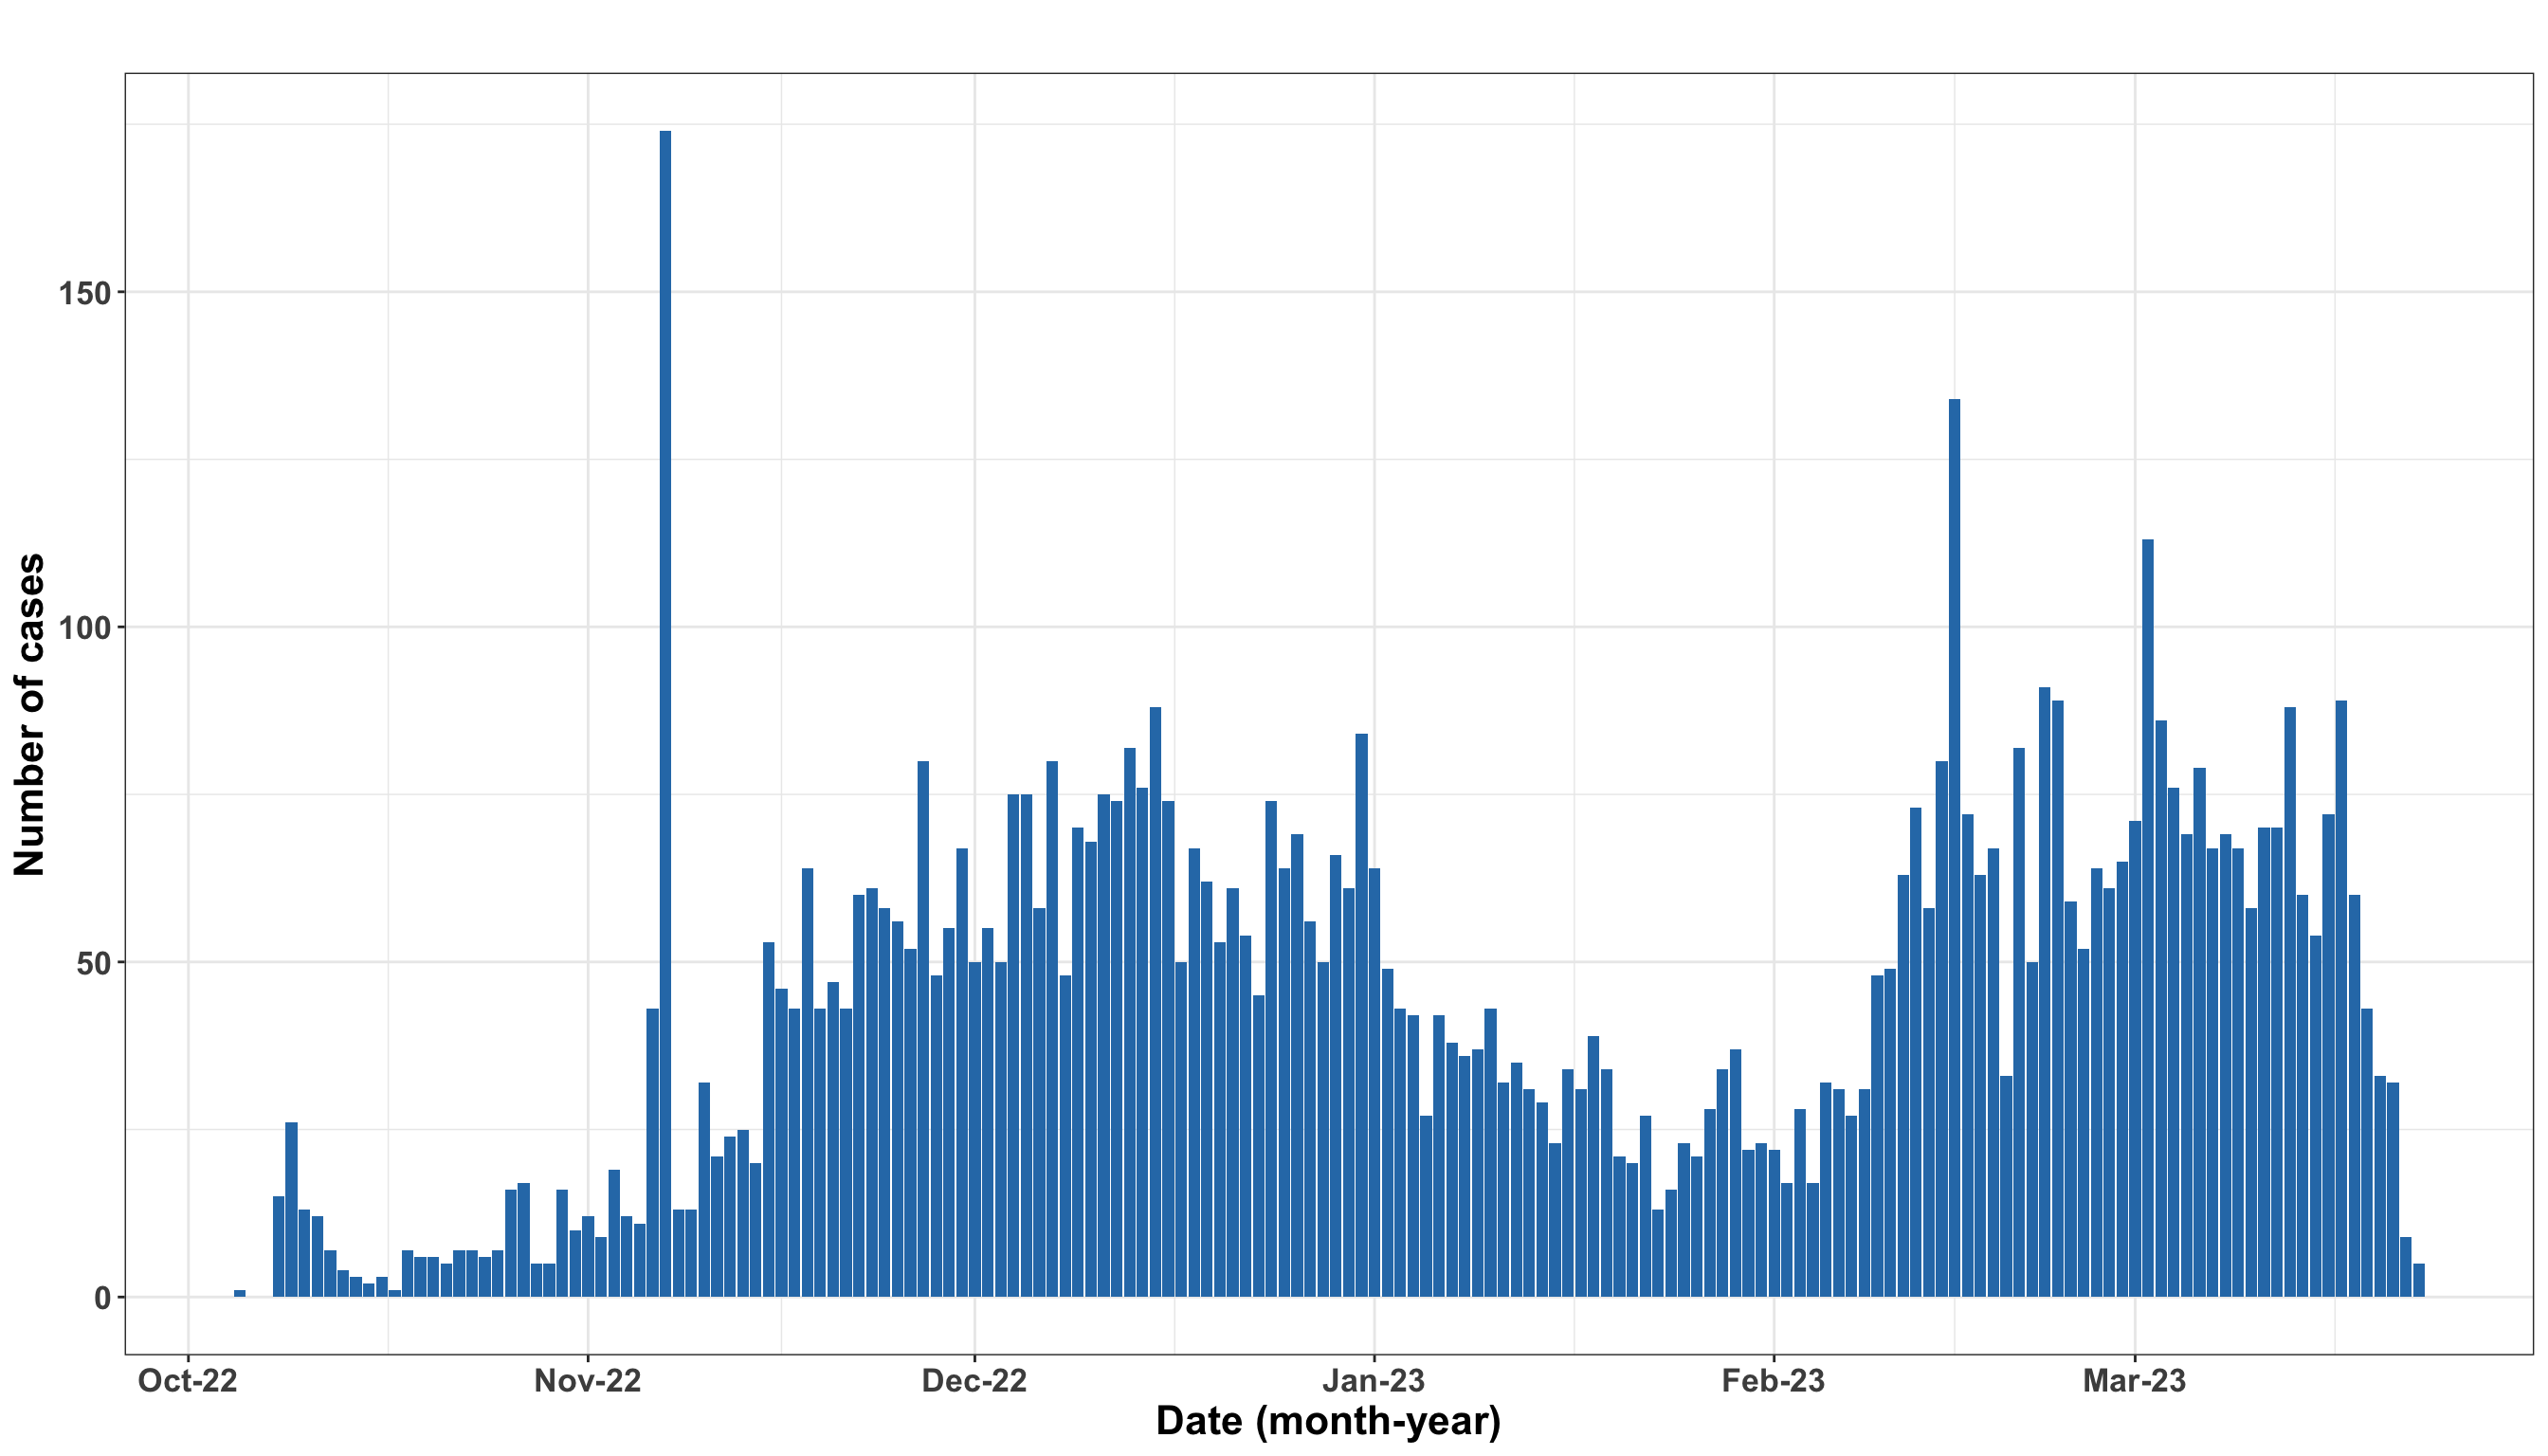
\includegraphics{_main_files/figure-latex/unnamed-chunk-4-1.pdf}

\hypertarget{demographic-distribution}{%
\section{Demographic distribution}\label{demographic-distribution}}

The stratification of these cases by age and sex is as shown:

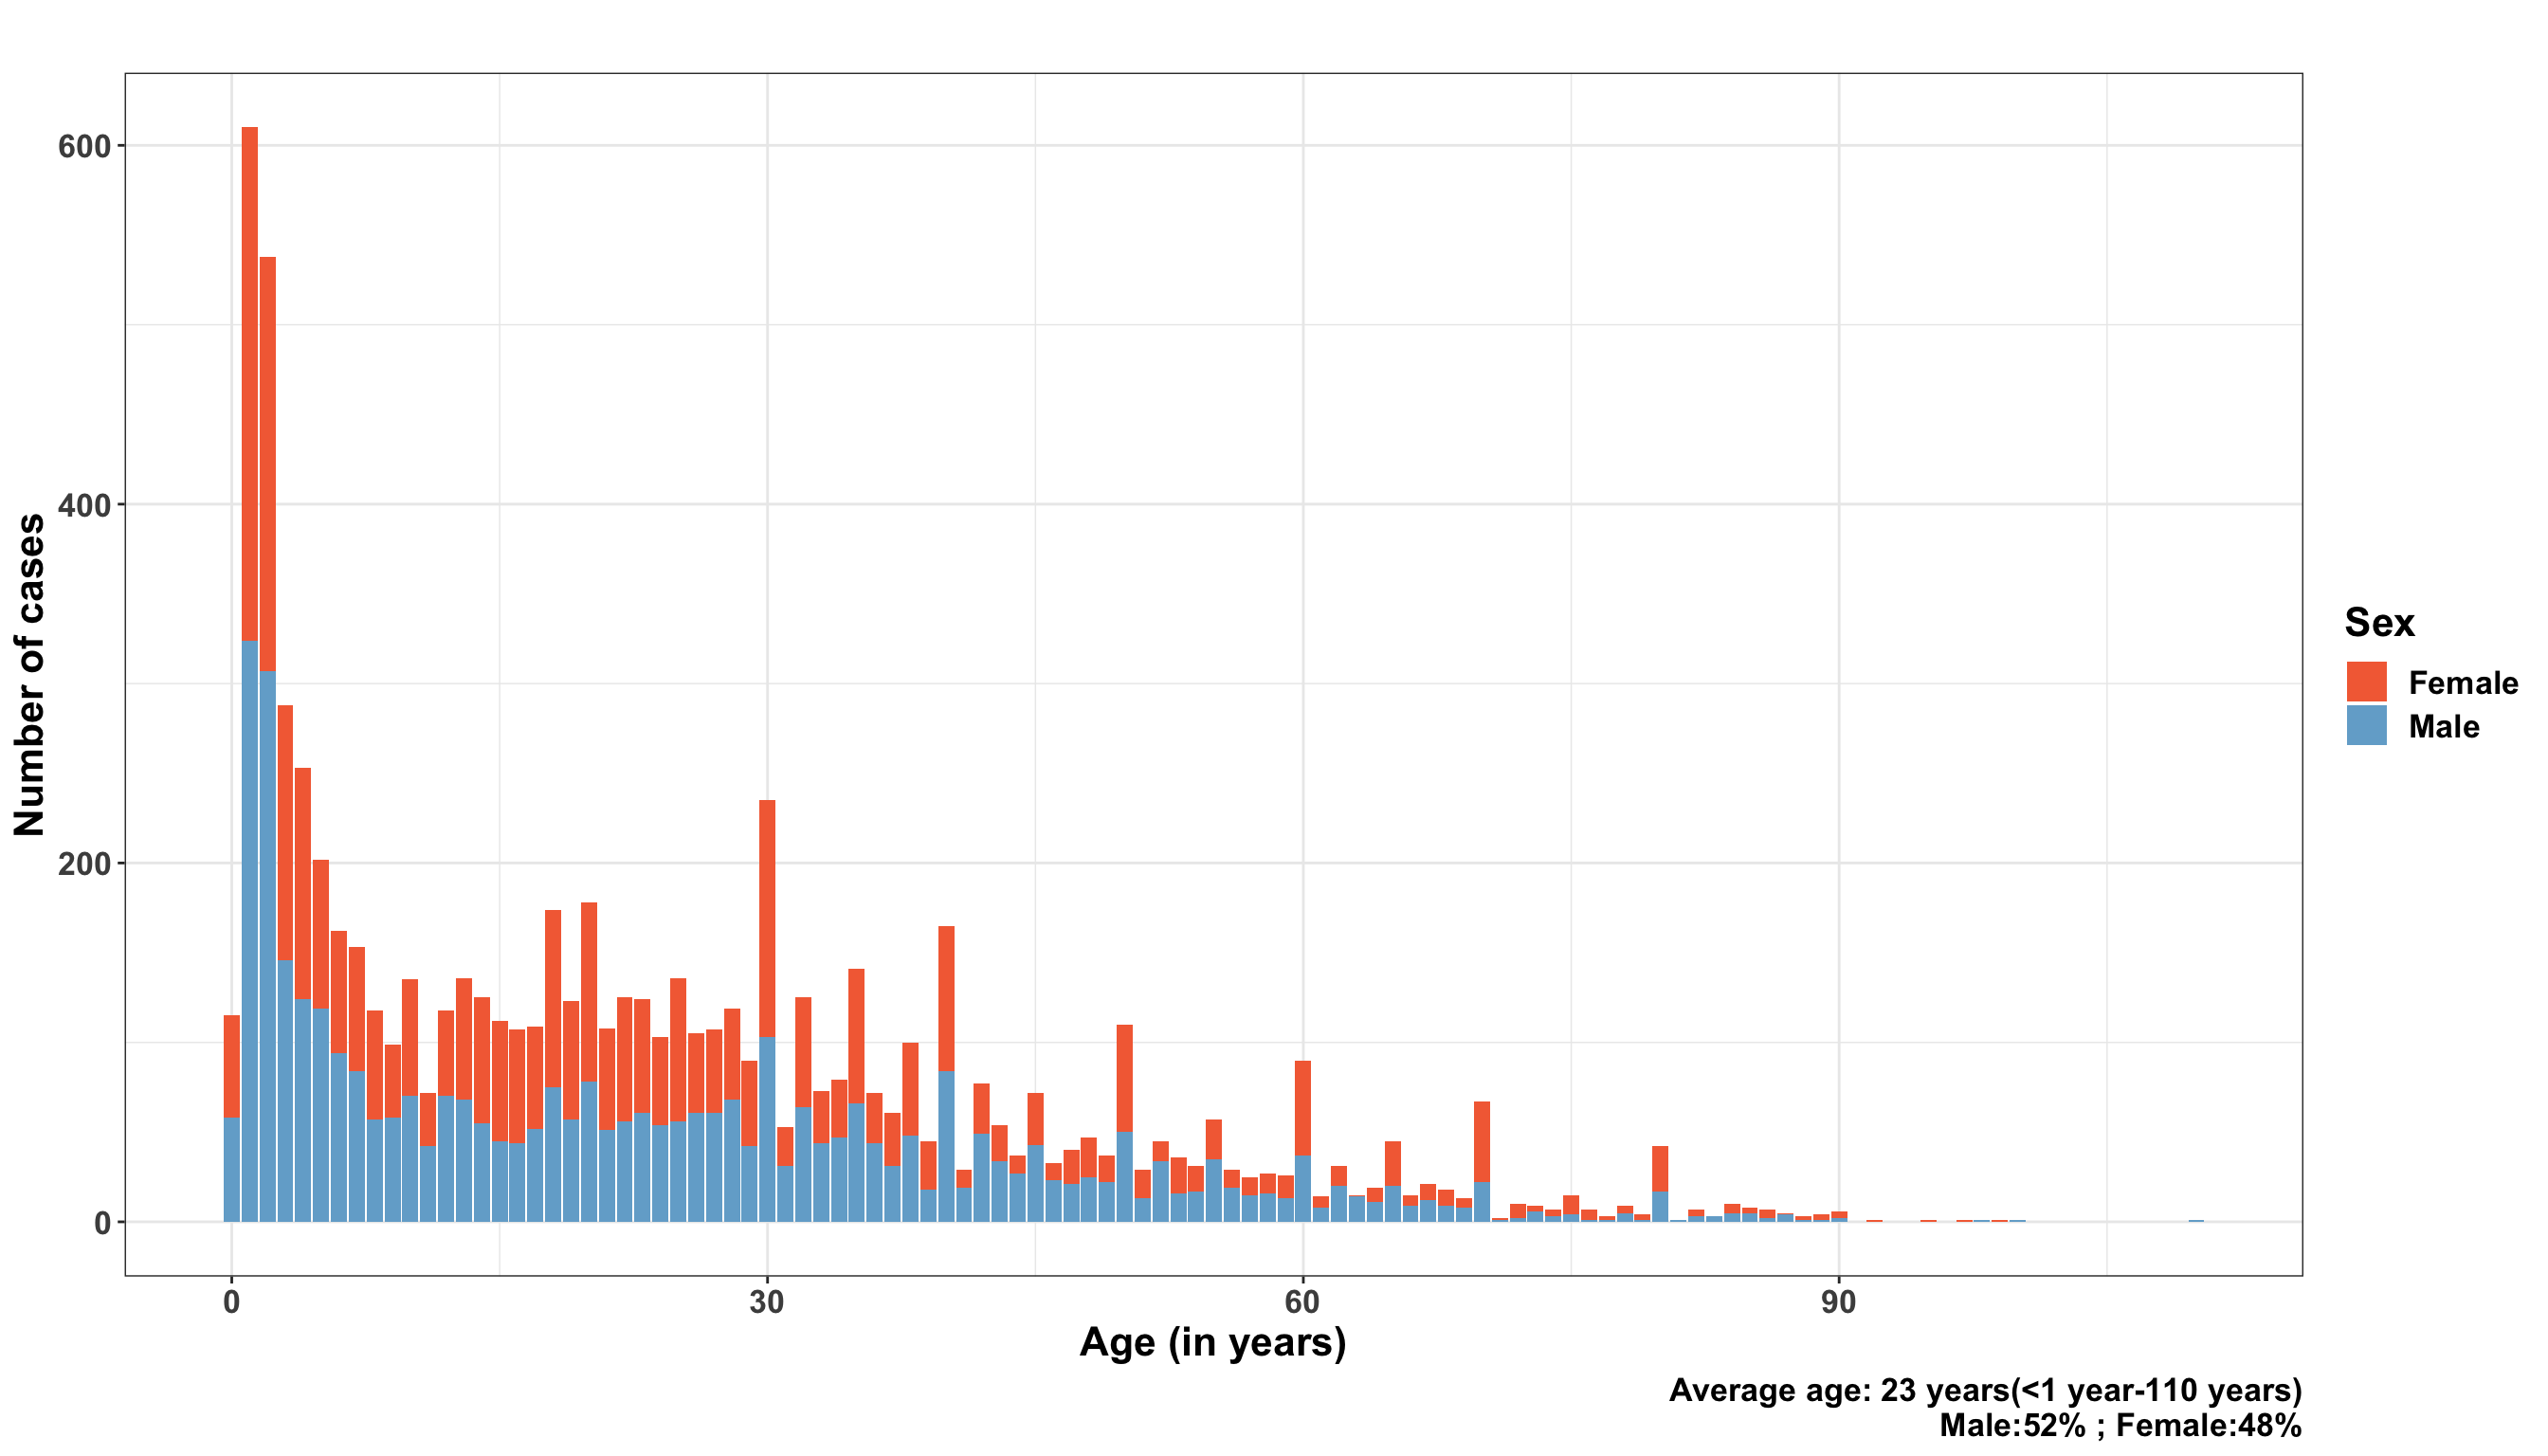
\includegraphics{_main_files/figure-latex/unnamed-chunk-6-1.pdf}

\hypertarget{spatial-distribution}{%
\section{Spatial distribution}\label{spatial-distribution}}

The spatial distribution of these cases at subcounty level is as shown:

\hypertarget{bomet}{%
\chapter{Bomet}\label{bomet}}

\hypertarget{cases-over-time-1}{%
\section{Cases over time}\label{cases-over-time-1}}

As at 2023-03-23, there were 6 cases reported in Bomet County.

This is shown in the graph below:

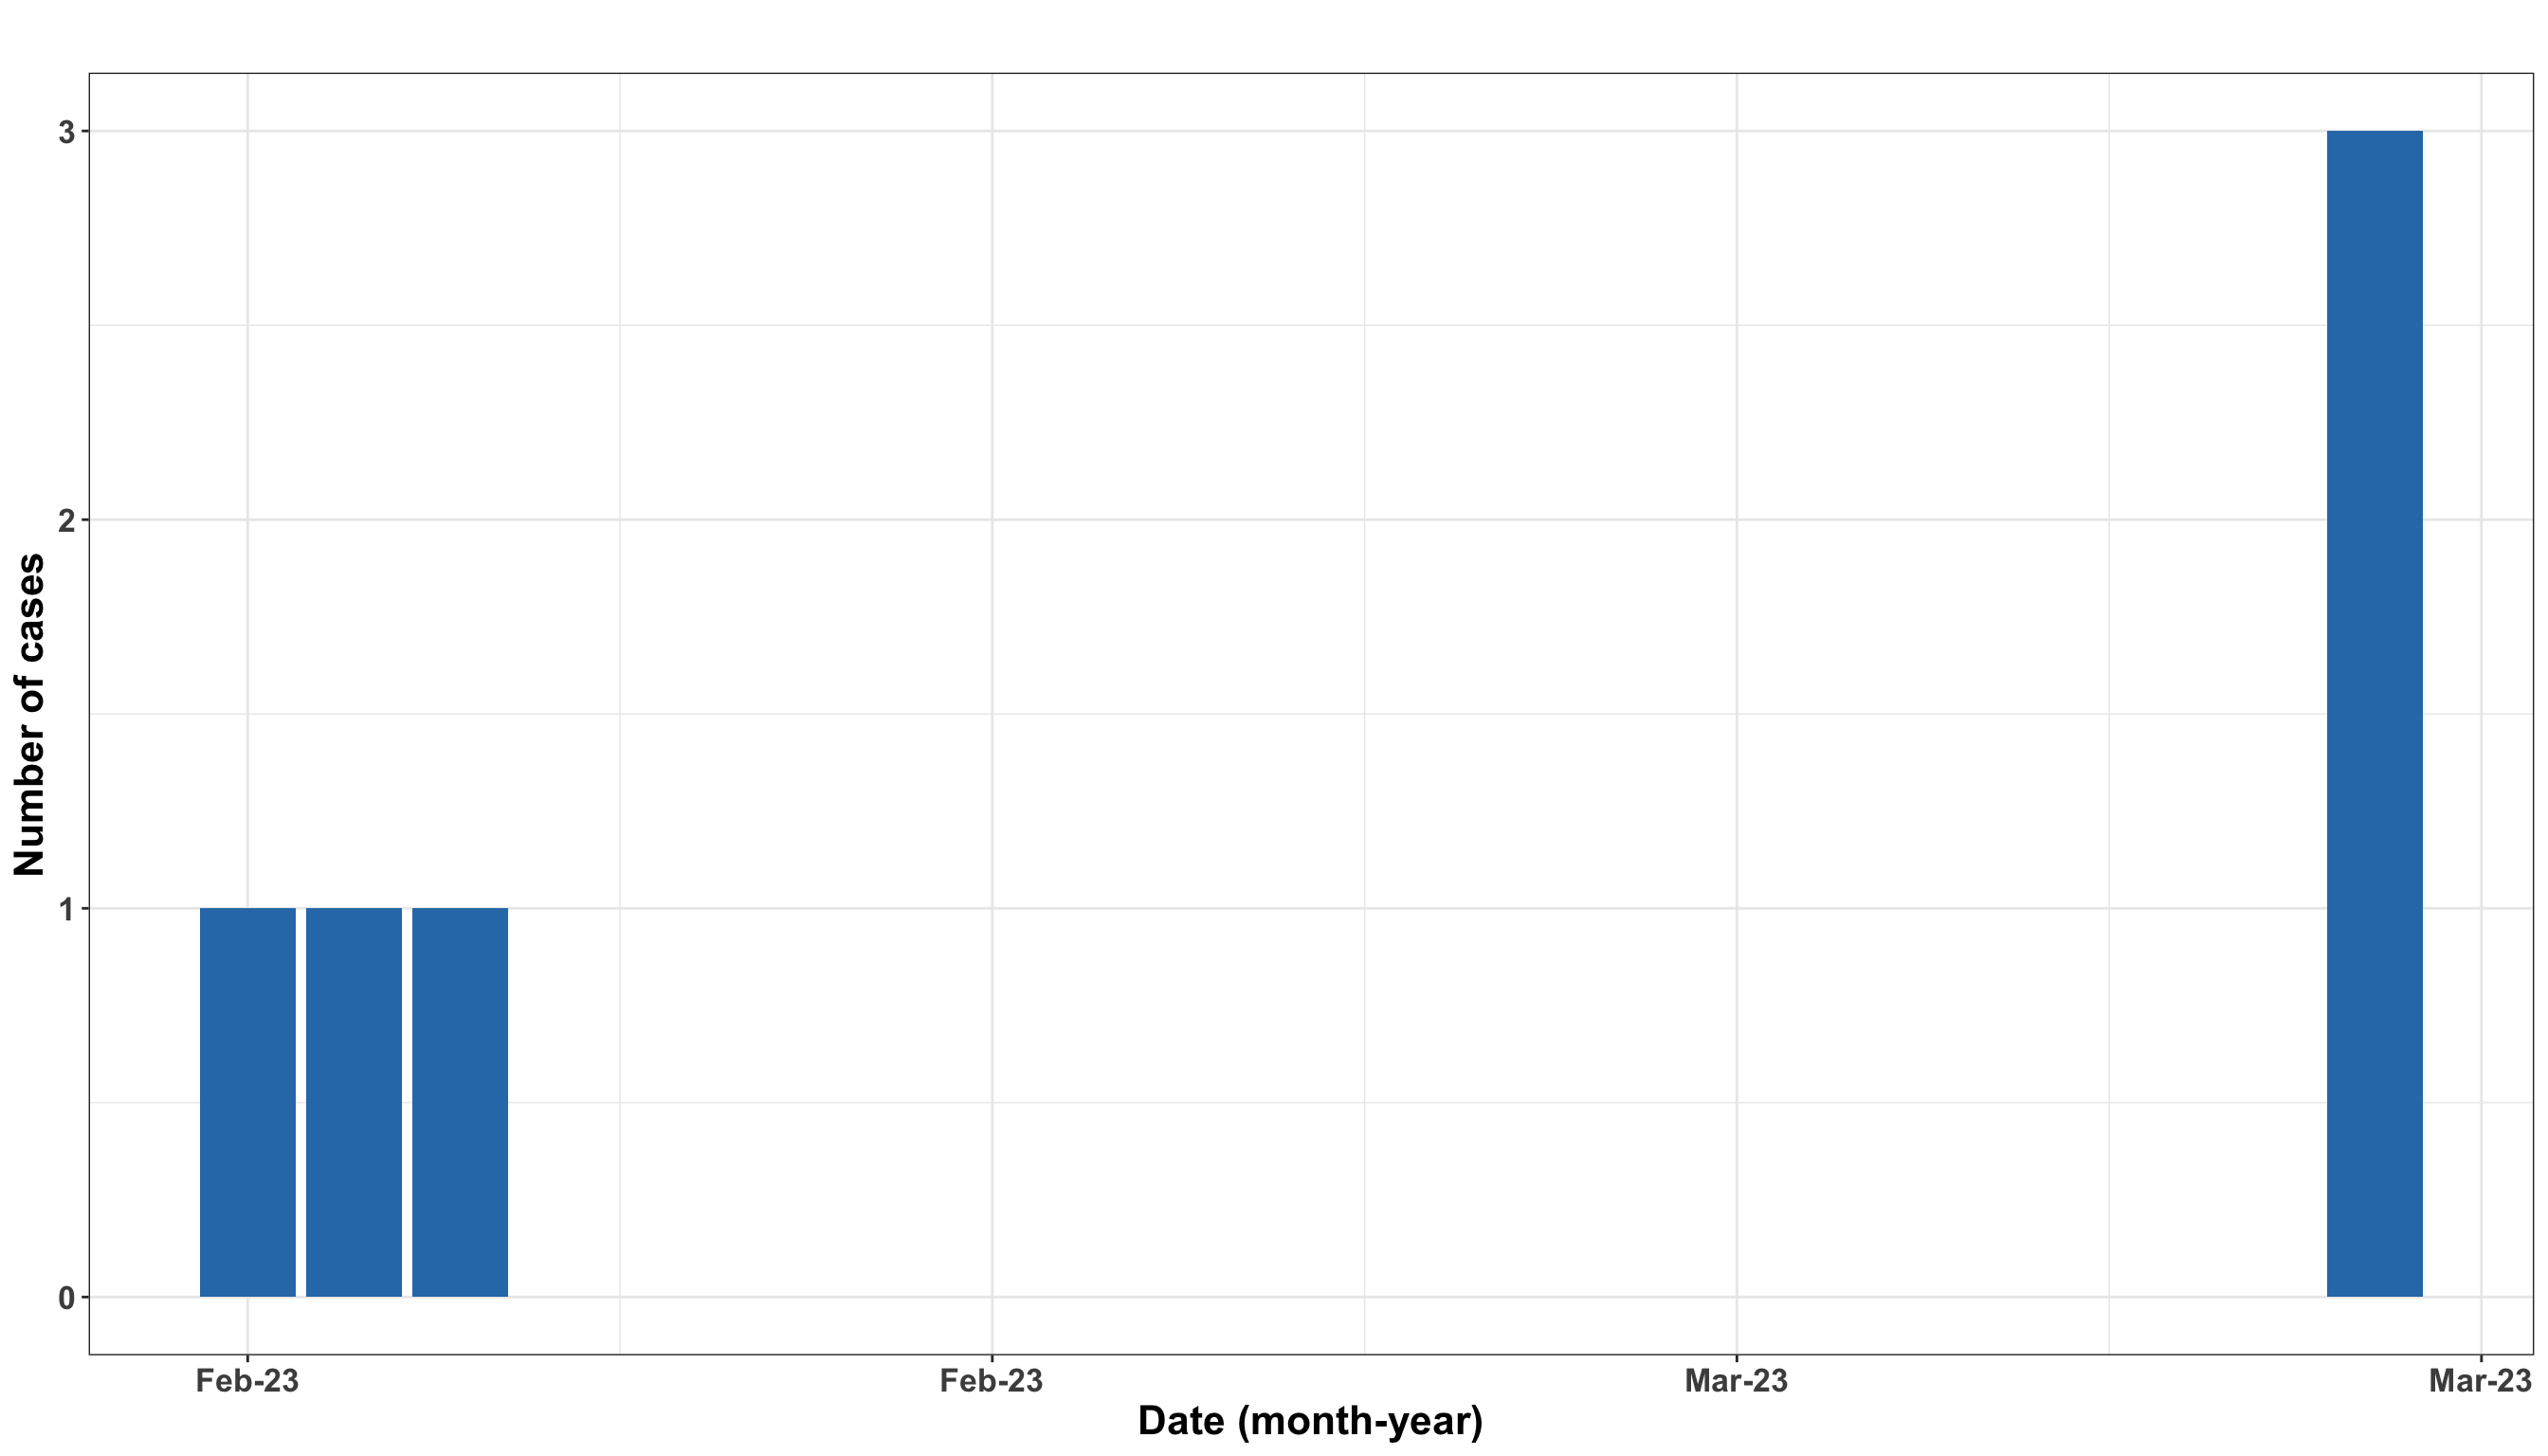
\includegraphics{_main_files/figure-latex/unnamed-chunk-10-1.pdf}

\hypertarget{demographic-distribution-1}{%
\section{Demographic distribution}\label{demographic-distribution-1}}

The stratification of these cases by age and sex is as shown:

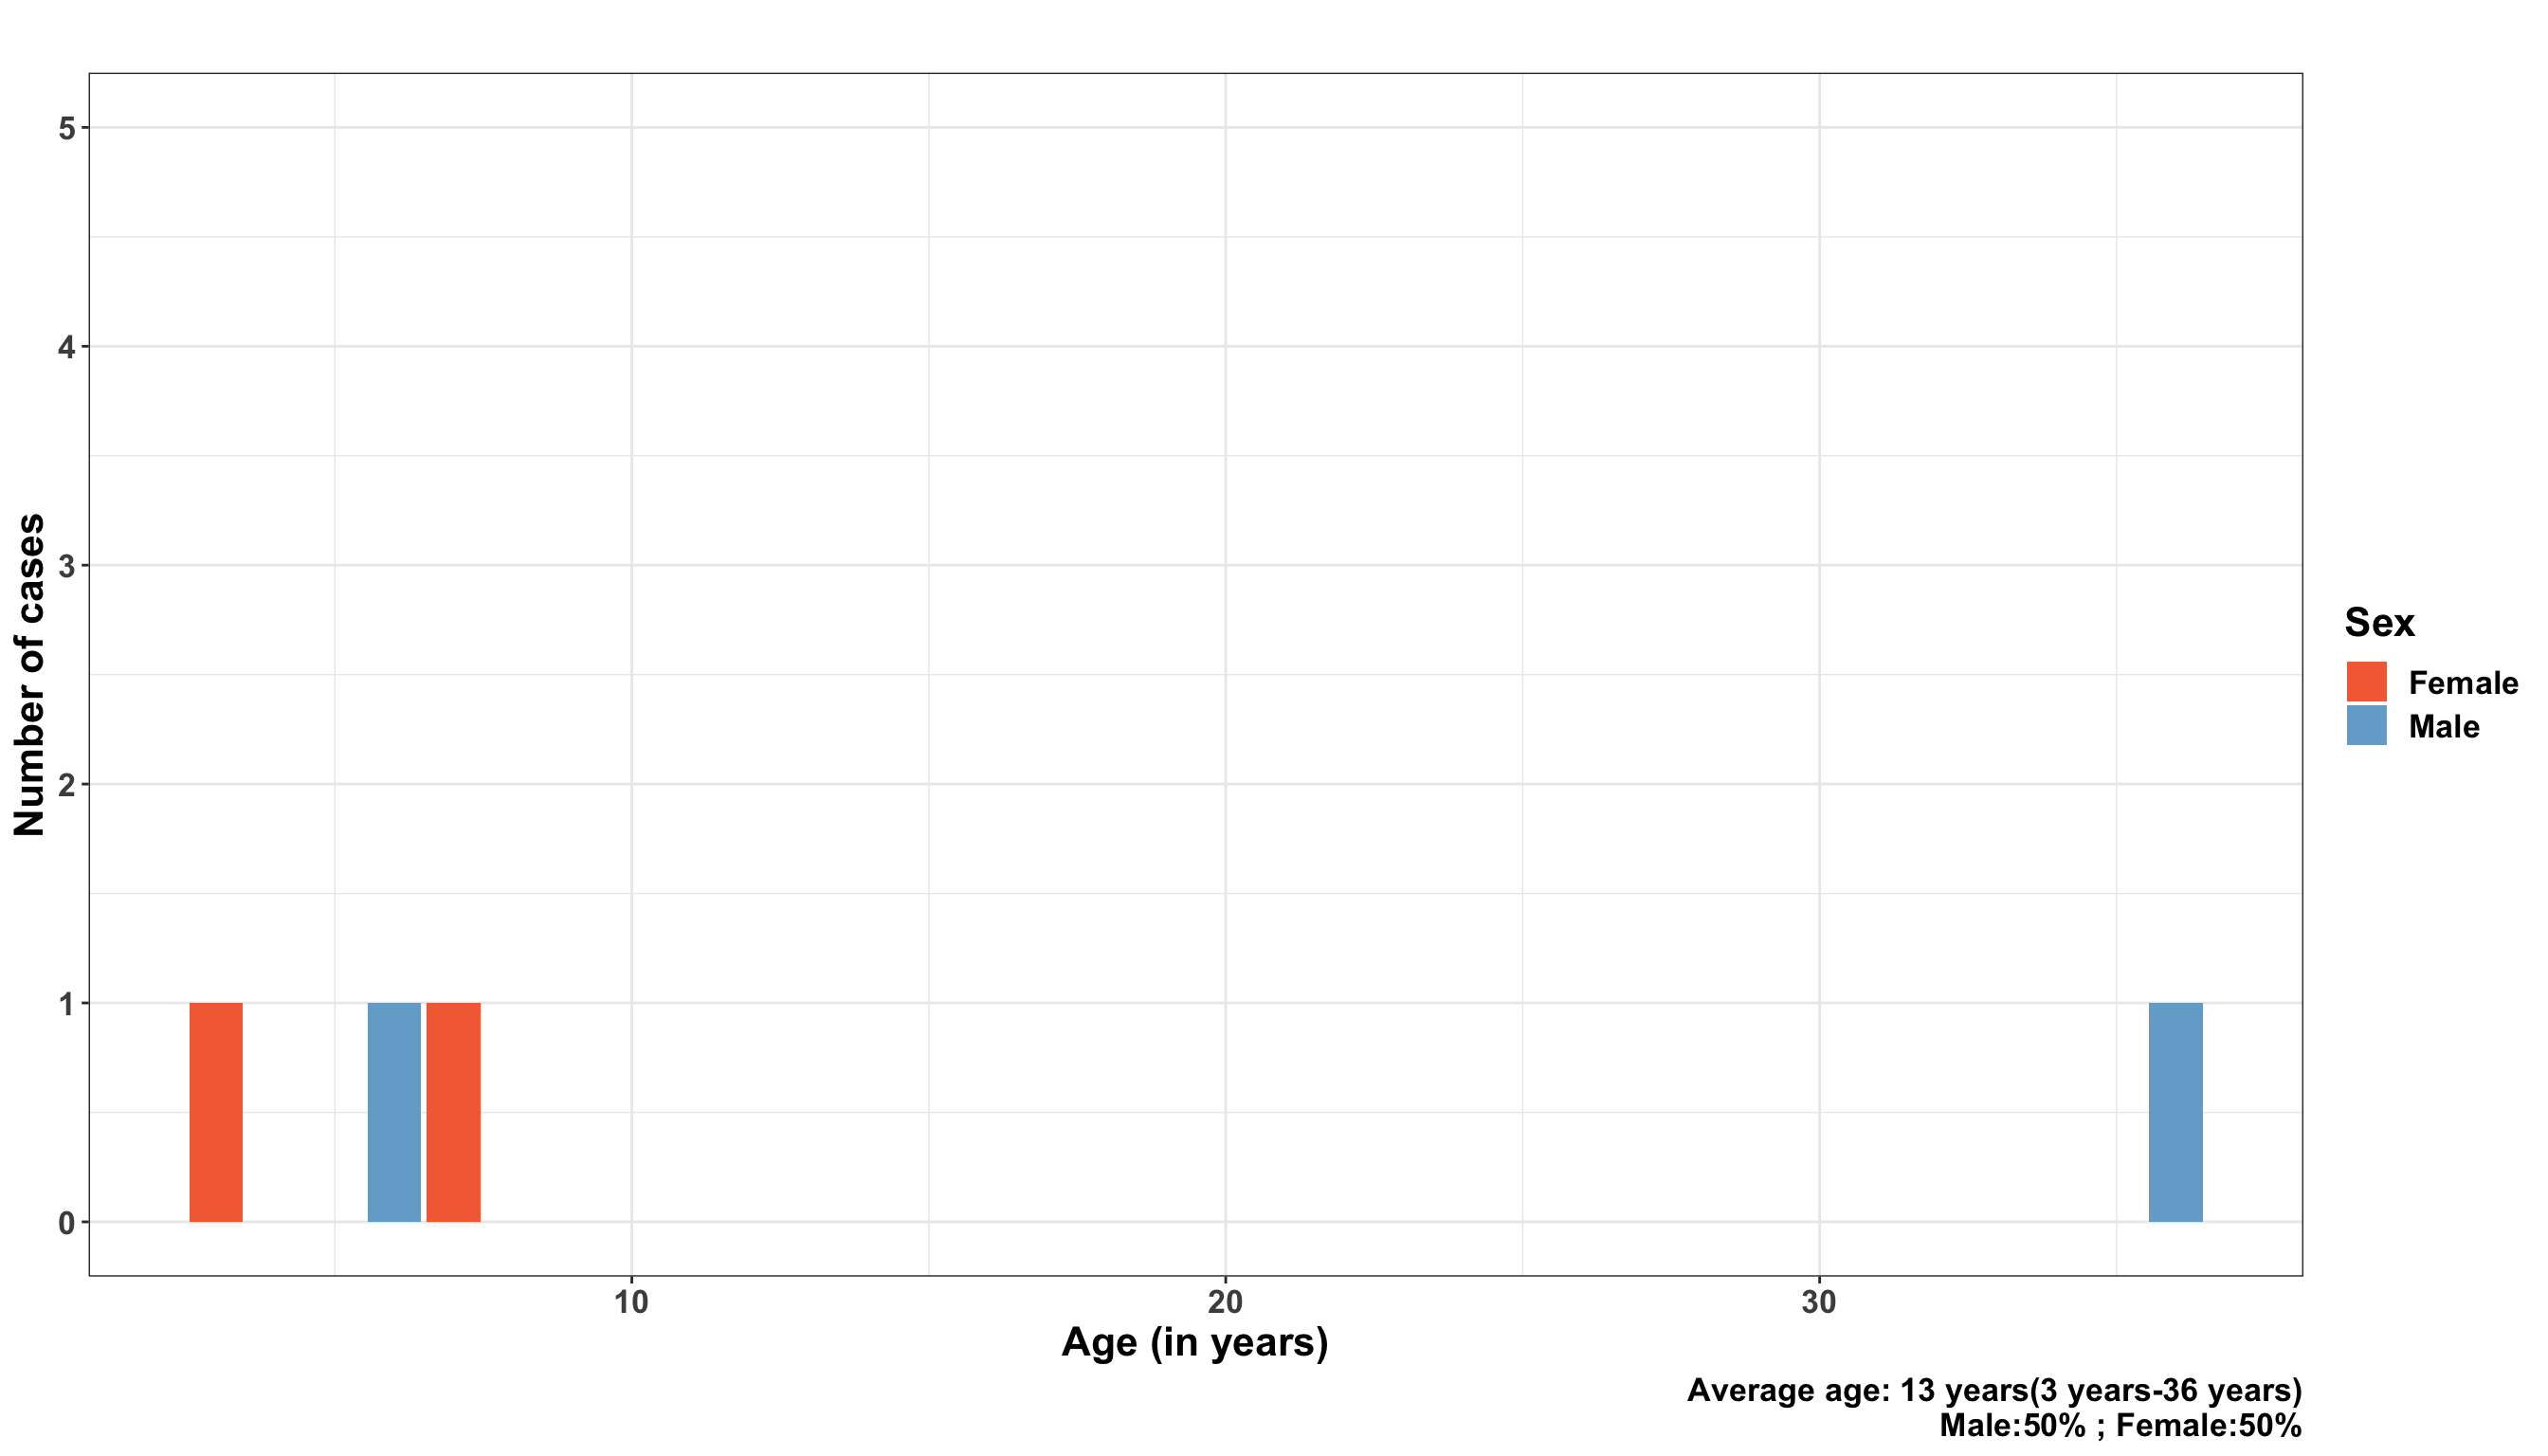
\includegraphics{_main_files/figure-latex/unnamed-chunk-12-1.pdf}

\hypertarget{spatial-distribution-1}{%
\section{Spatial distribution}\label{spatial-distribution-1}}

The spatial distribution of these cases at subcounty level is as shown:

\hypertarget{garissa}{%
\chapter{Garissa}\label{garissa}}

\hypertarget{cases-over-time-2}{%
\section{Cases over time}\label{cases-over-time-2}}

As at 2023-03-23, there were 2163 cases reported in Garissa County.

This is shown in the graph below:

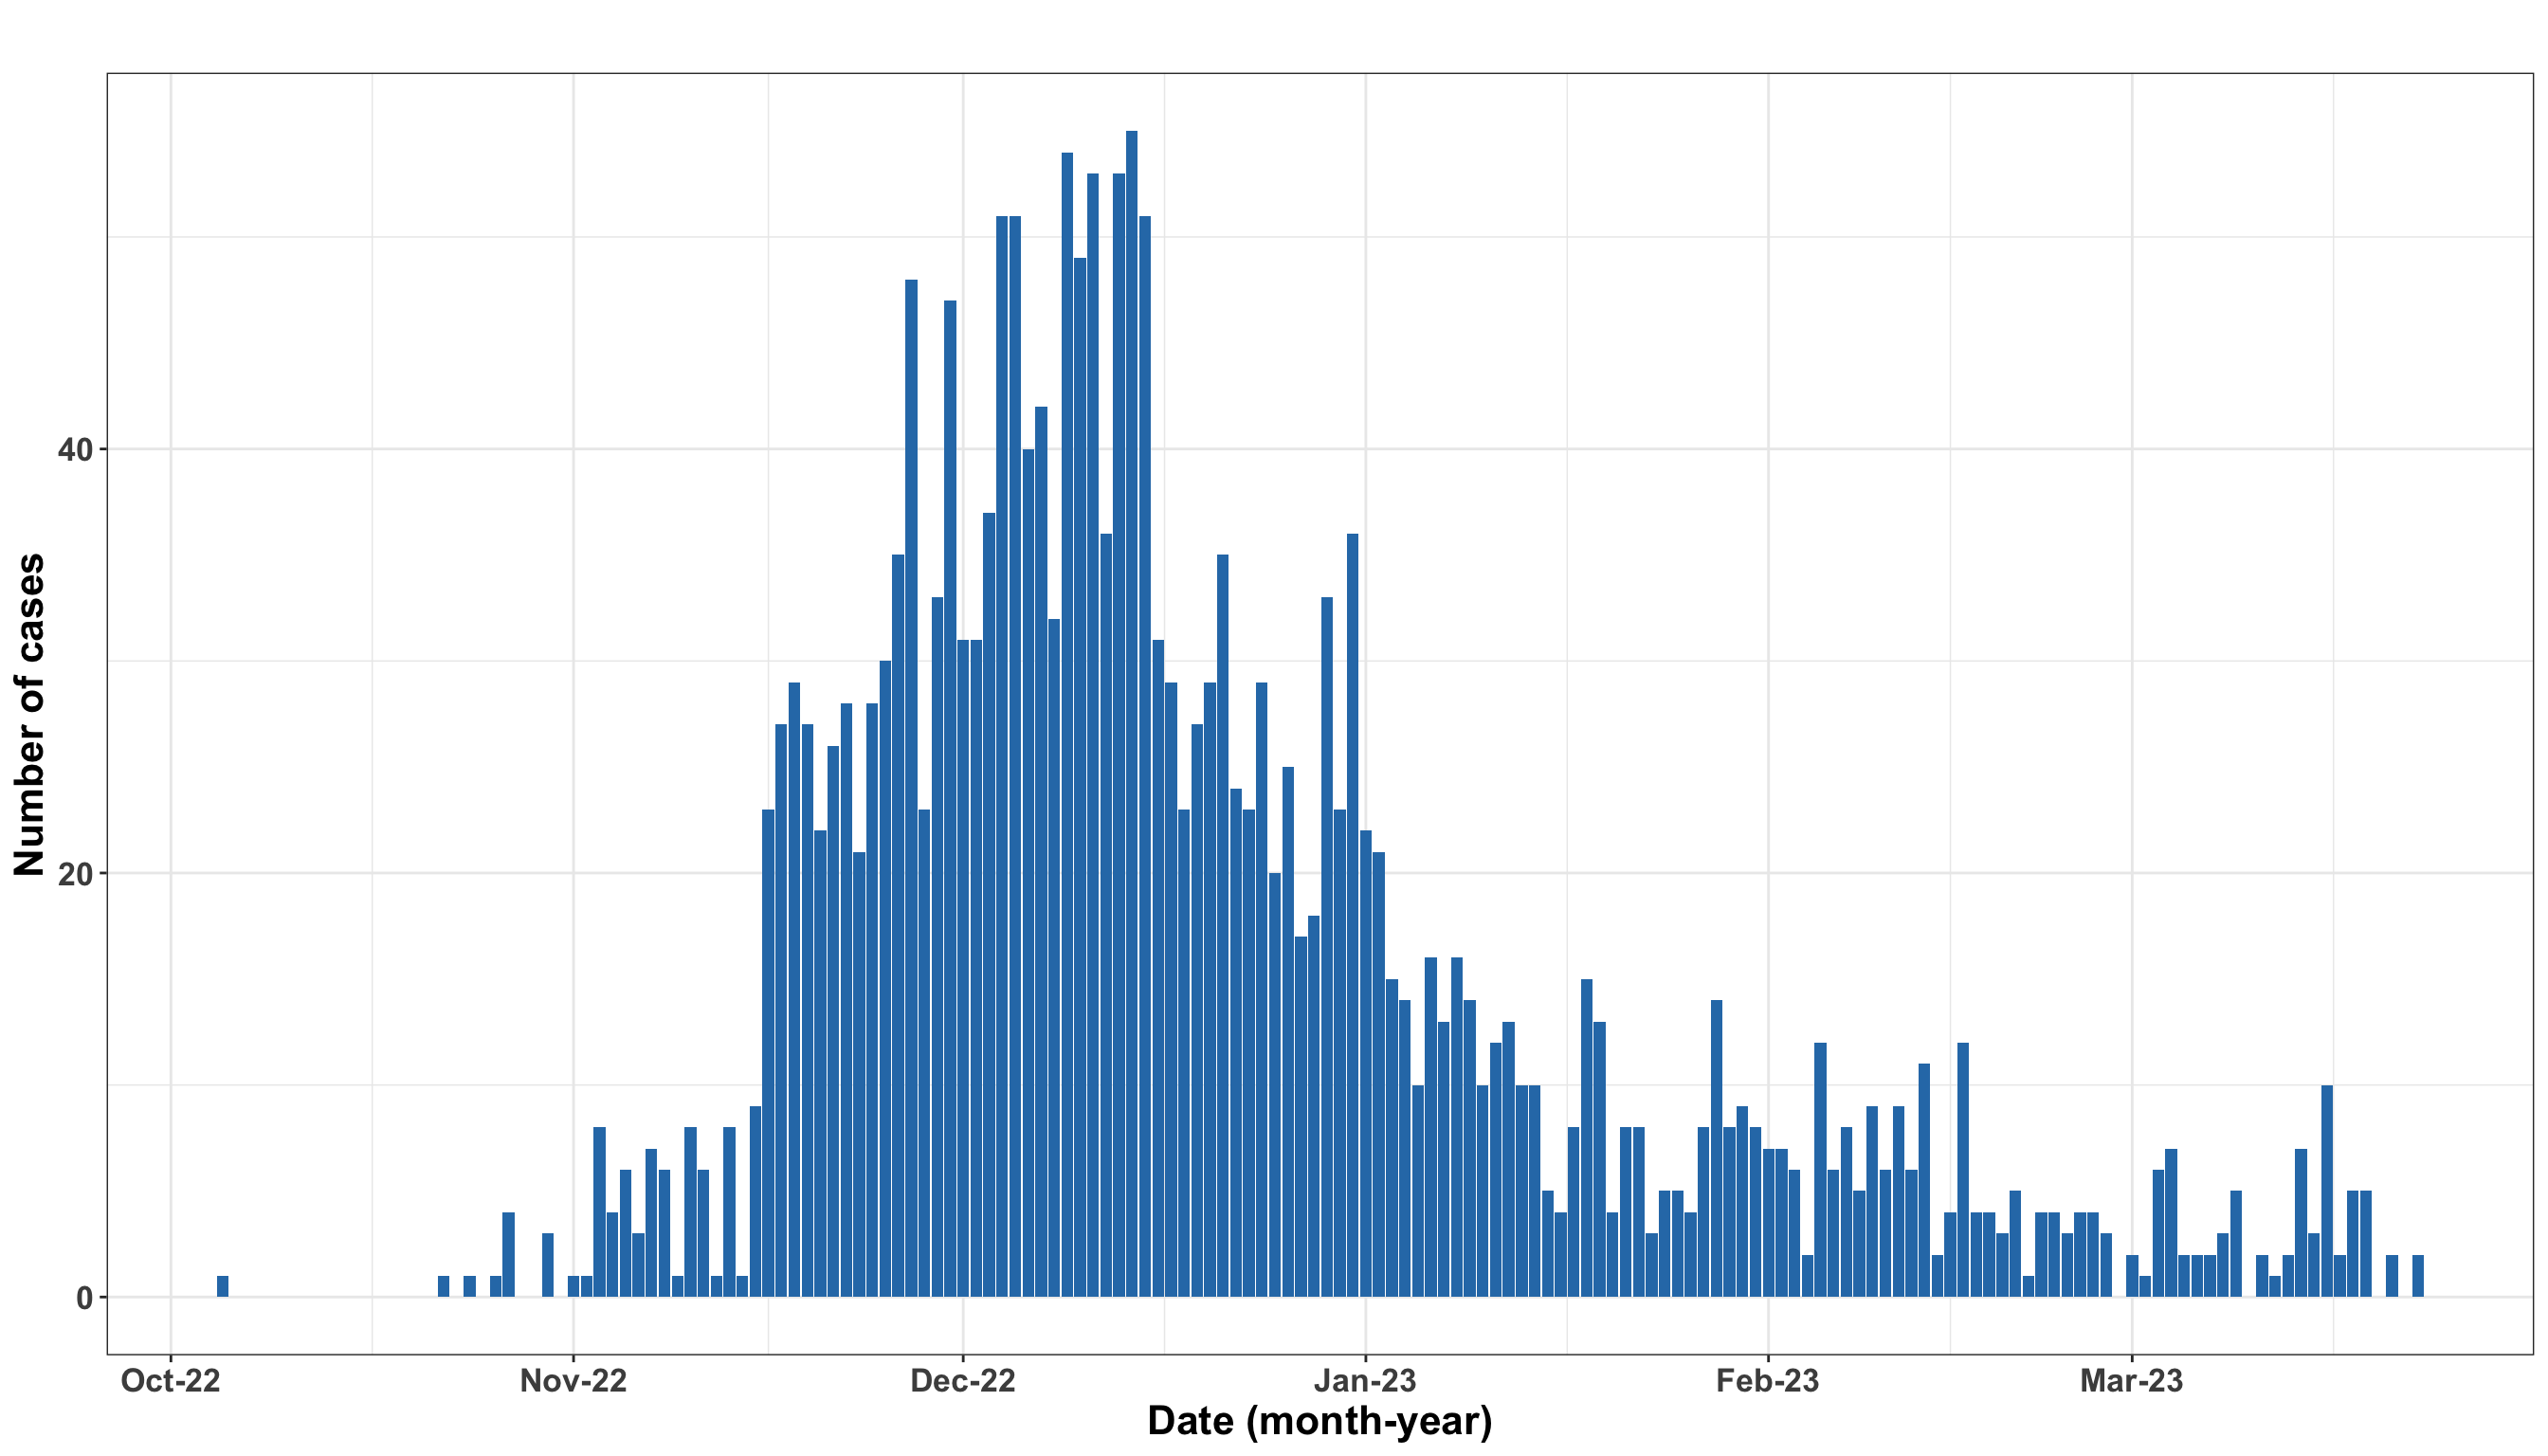
\includegraphics{_main_files/figure-latex/unnamed-chunk-16-1.pdf}

\hypertarget{demographic-distribution-2}{%
\section{Demographic distribution}\label{demographic-distribution-2}}

The stratification of these cases by age and sex is as shown:

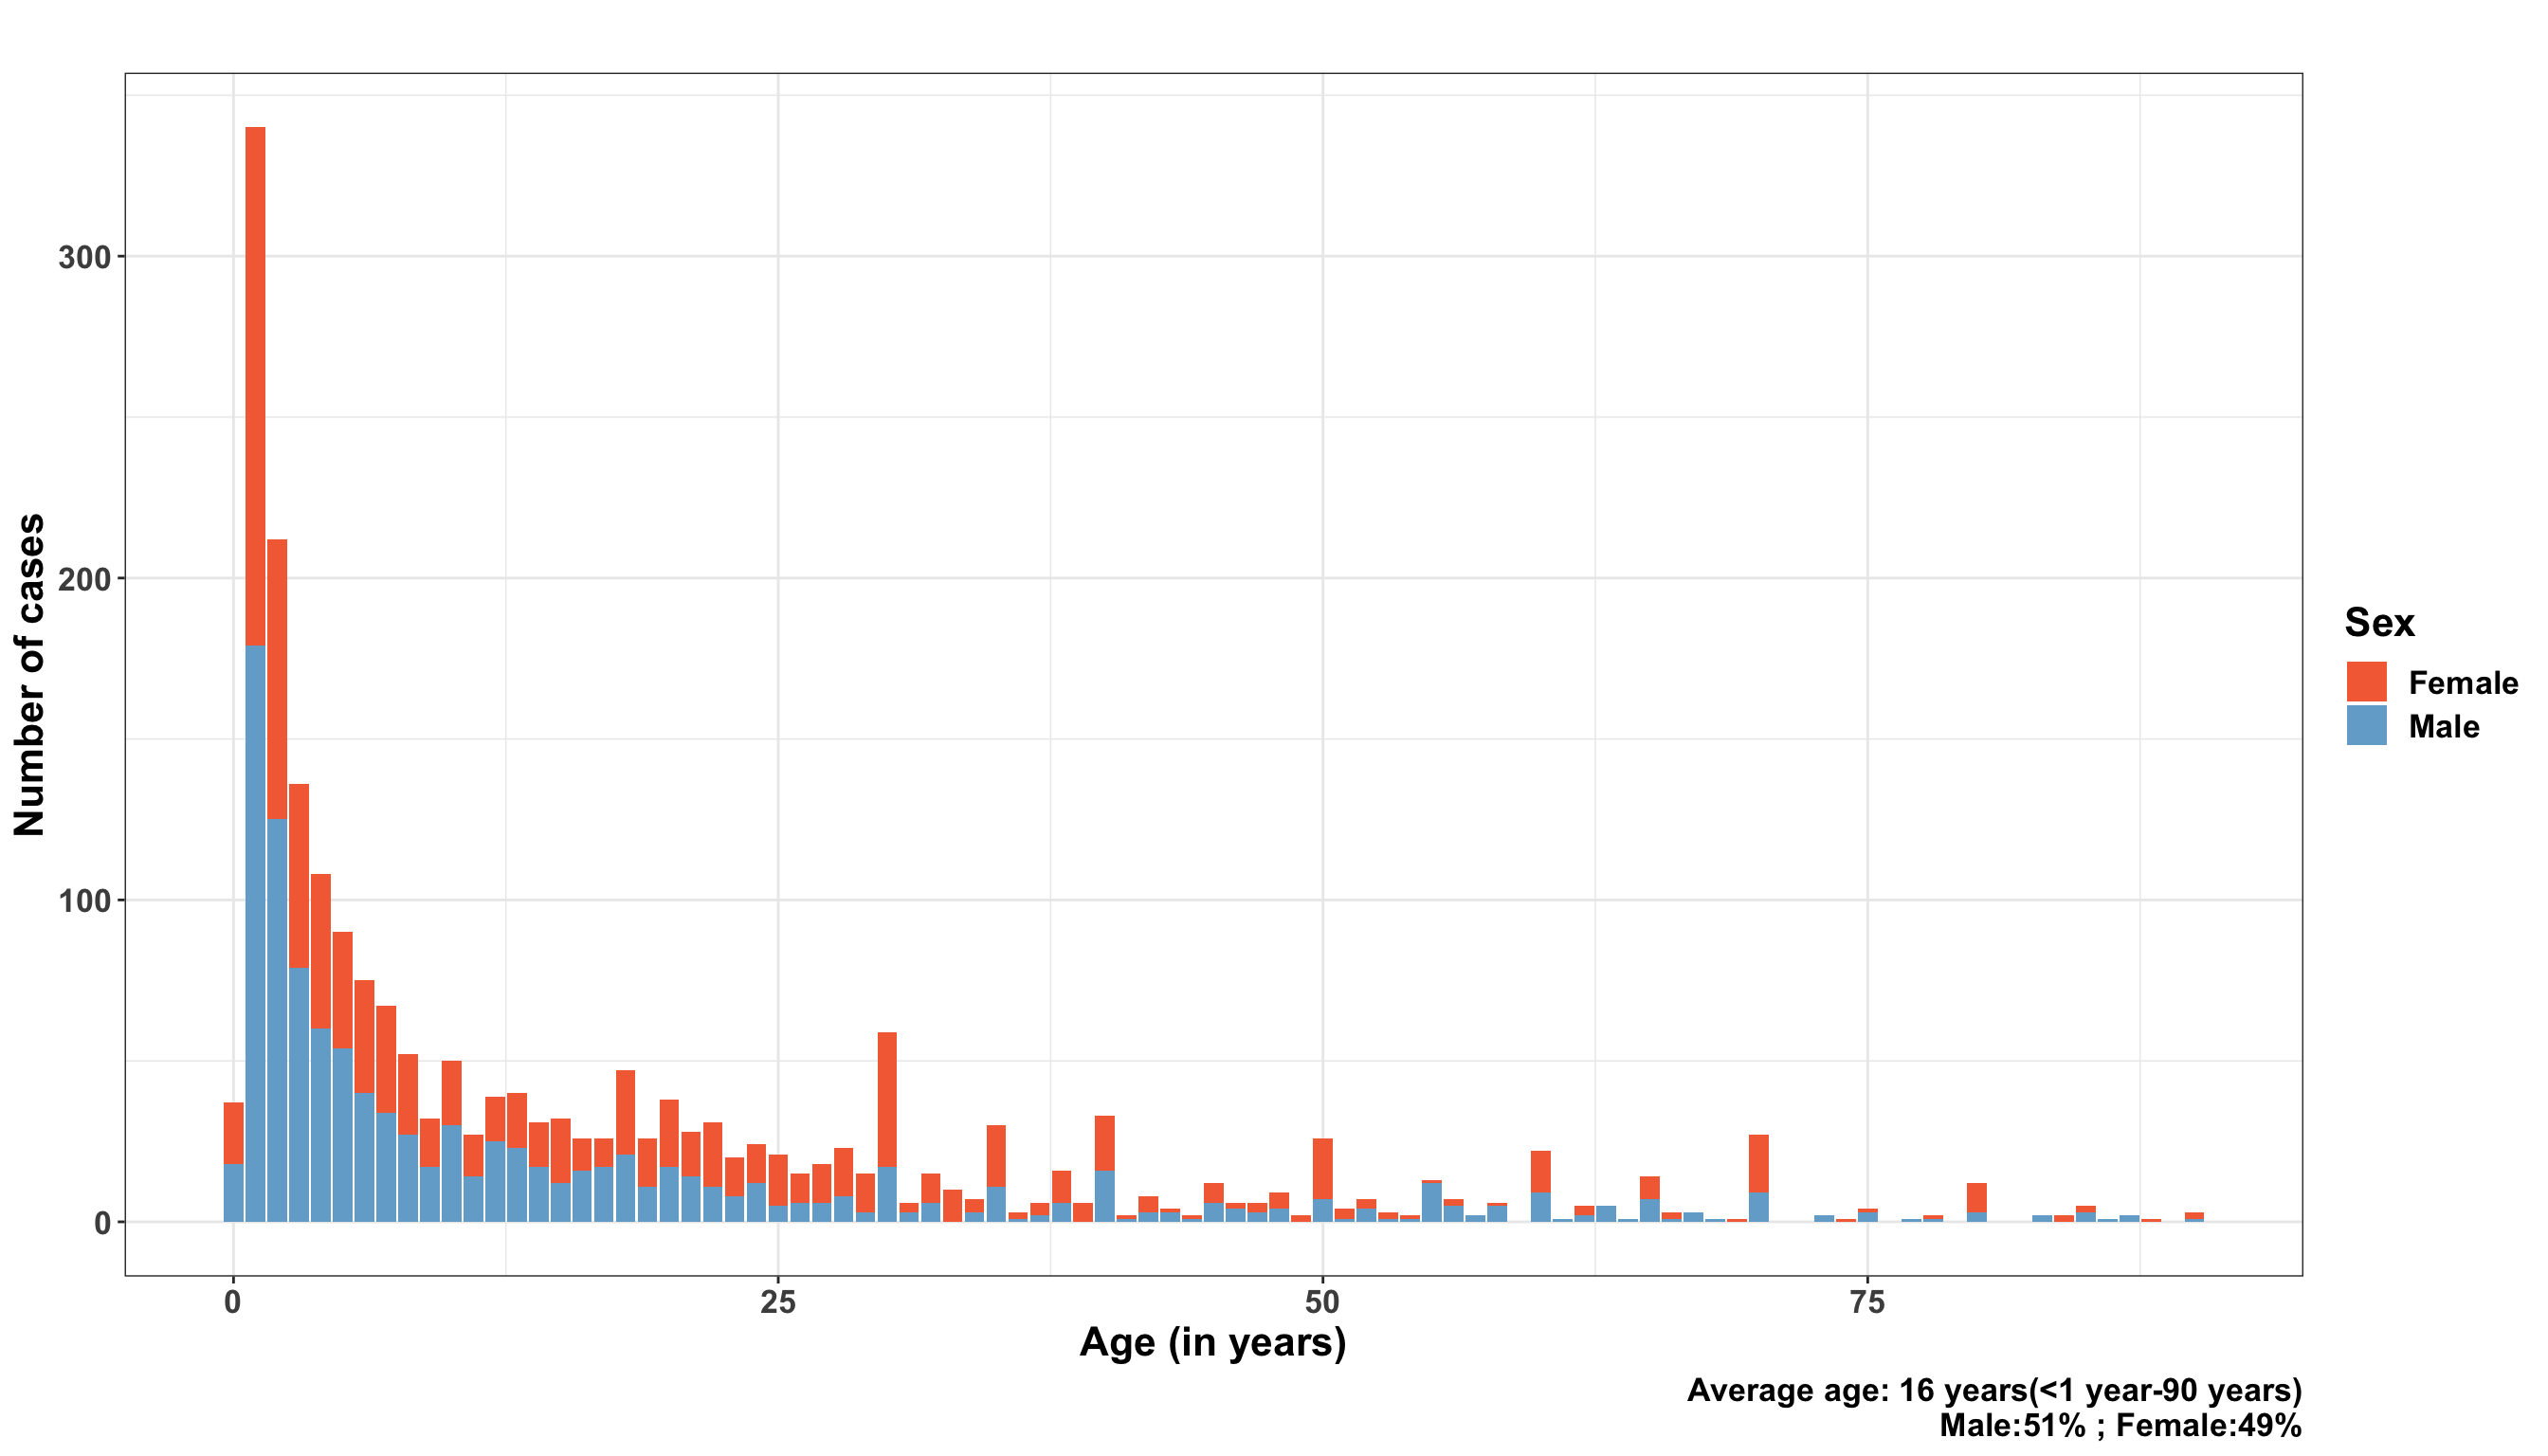
\includegraphics{_main_files/figure-latex/unnamed-chunk-18-1.pdf}

\hypertarget{spatial-distribution-2}{%
\section{Spatial distribution}\label{spatial-distribution-2}}

The spatial distribution of these cases at subcounty level is as shown:

\hypertarget{homa-bay}{%
\chapter{Homa Bay}\label{homa-bay}}

\hypertarget{cases-over-time-3}{%
\section{Cases over time}\label{cases-over-time-3}}

As at 2023-03-23, there were 51 cases reported in Homa Bay County.

This is shown in the graph below:

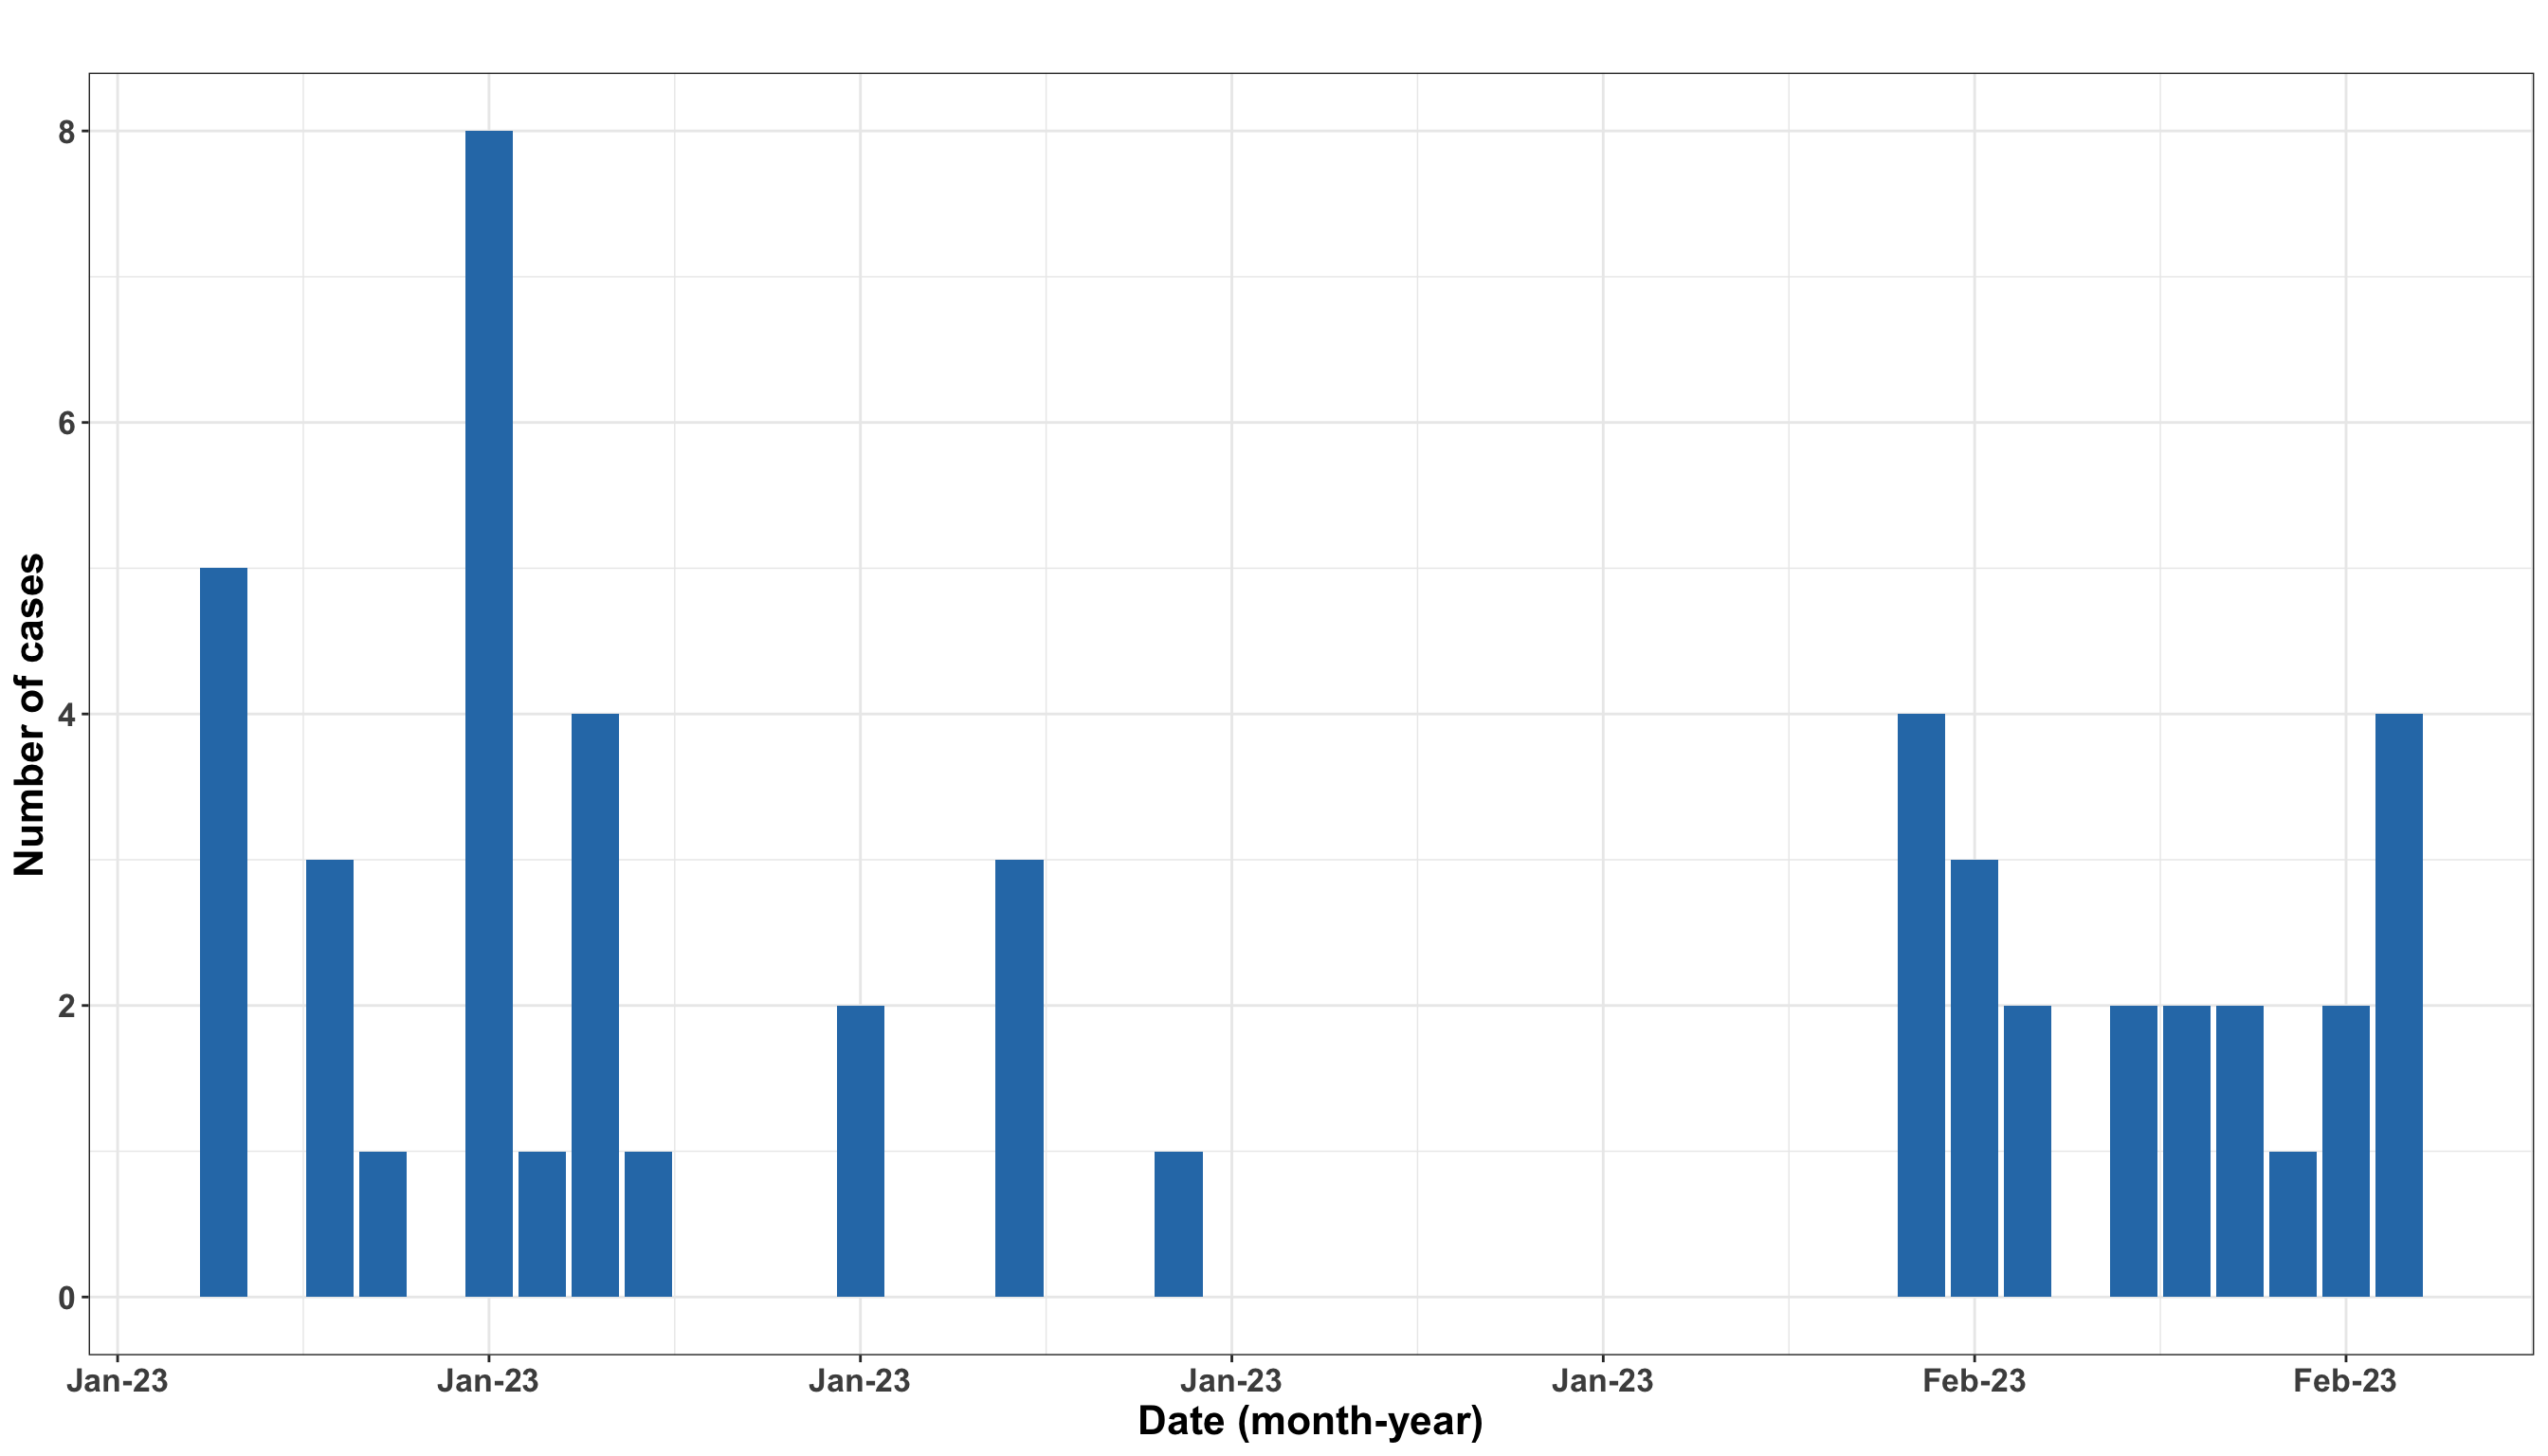
\includegraphics{_main_files/figure-latex/unnamed-chunk-22-1.pdf}

\hypertarget{demographic-distribution-3}{%
\section{Demographic distribution}\label{demographic-distribution-3}}

The stratification of these cases by age and sex is as shown:

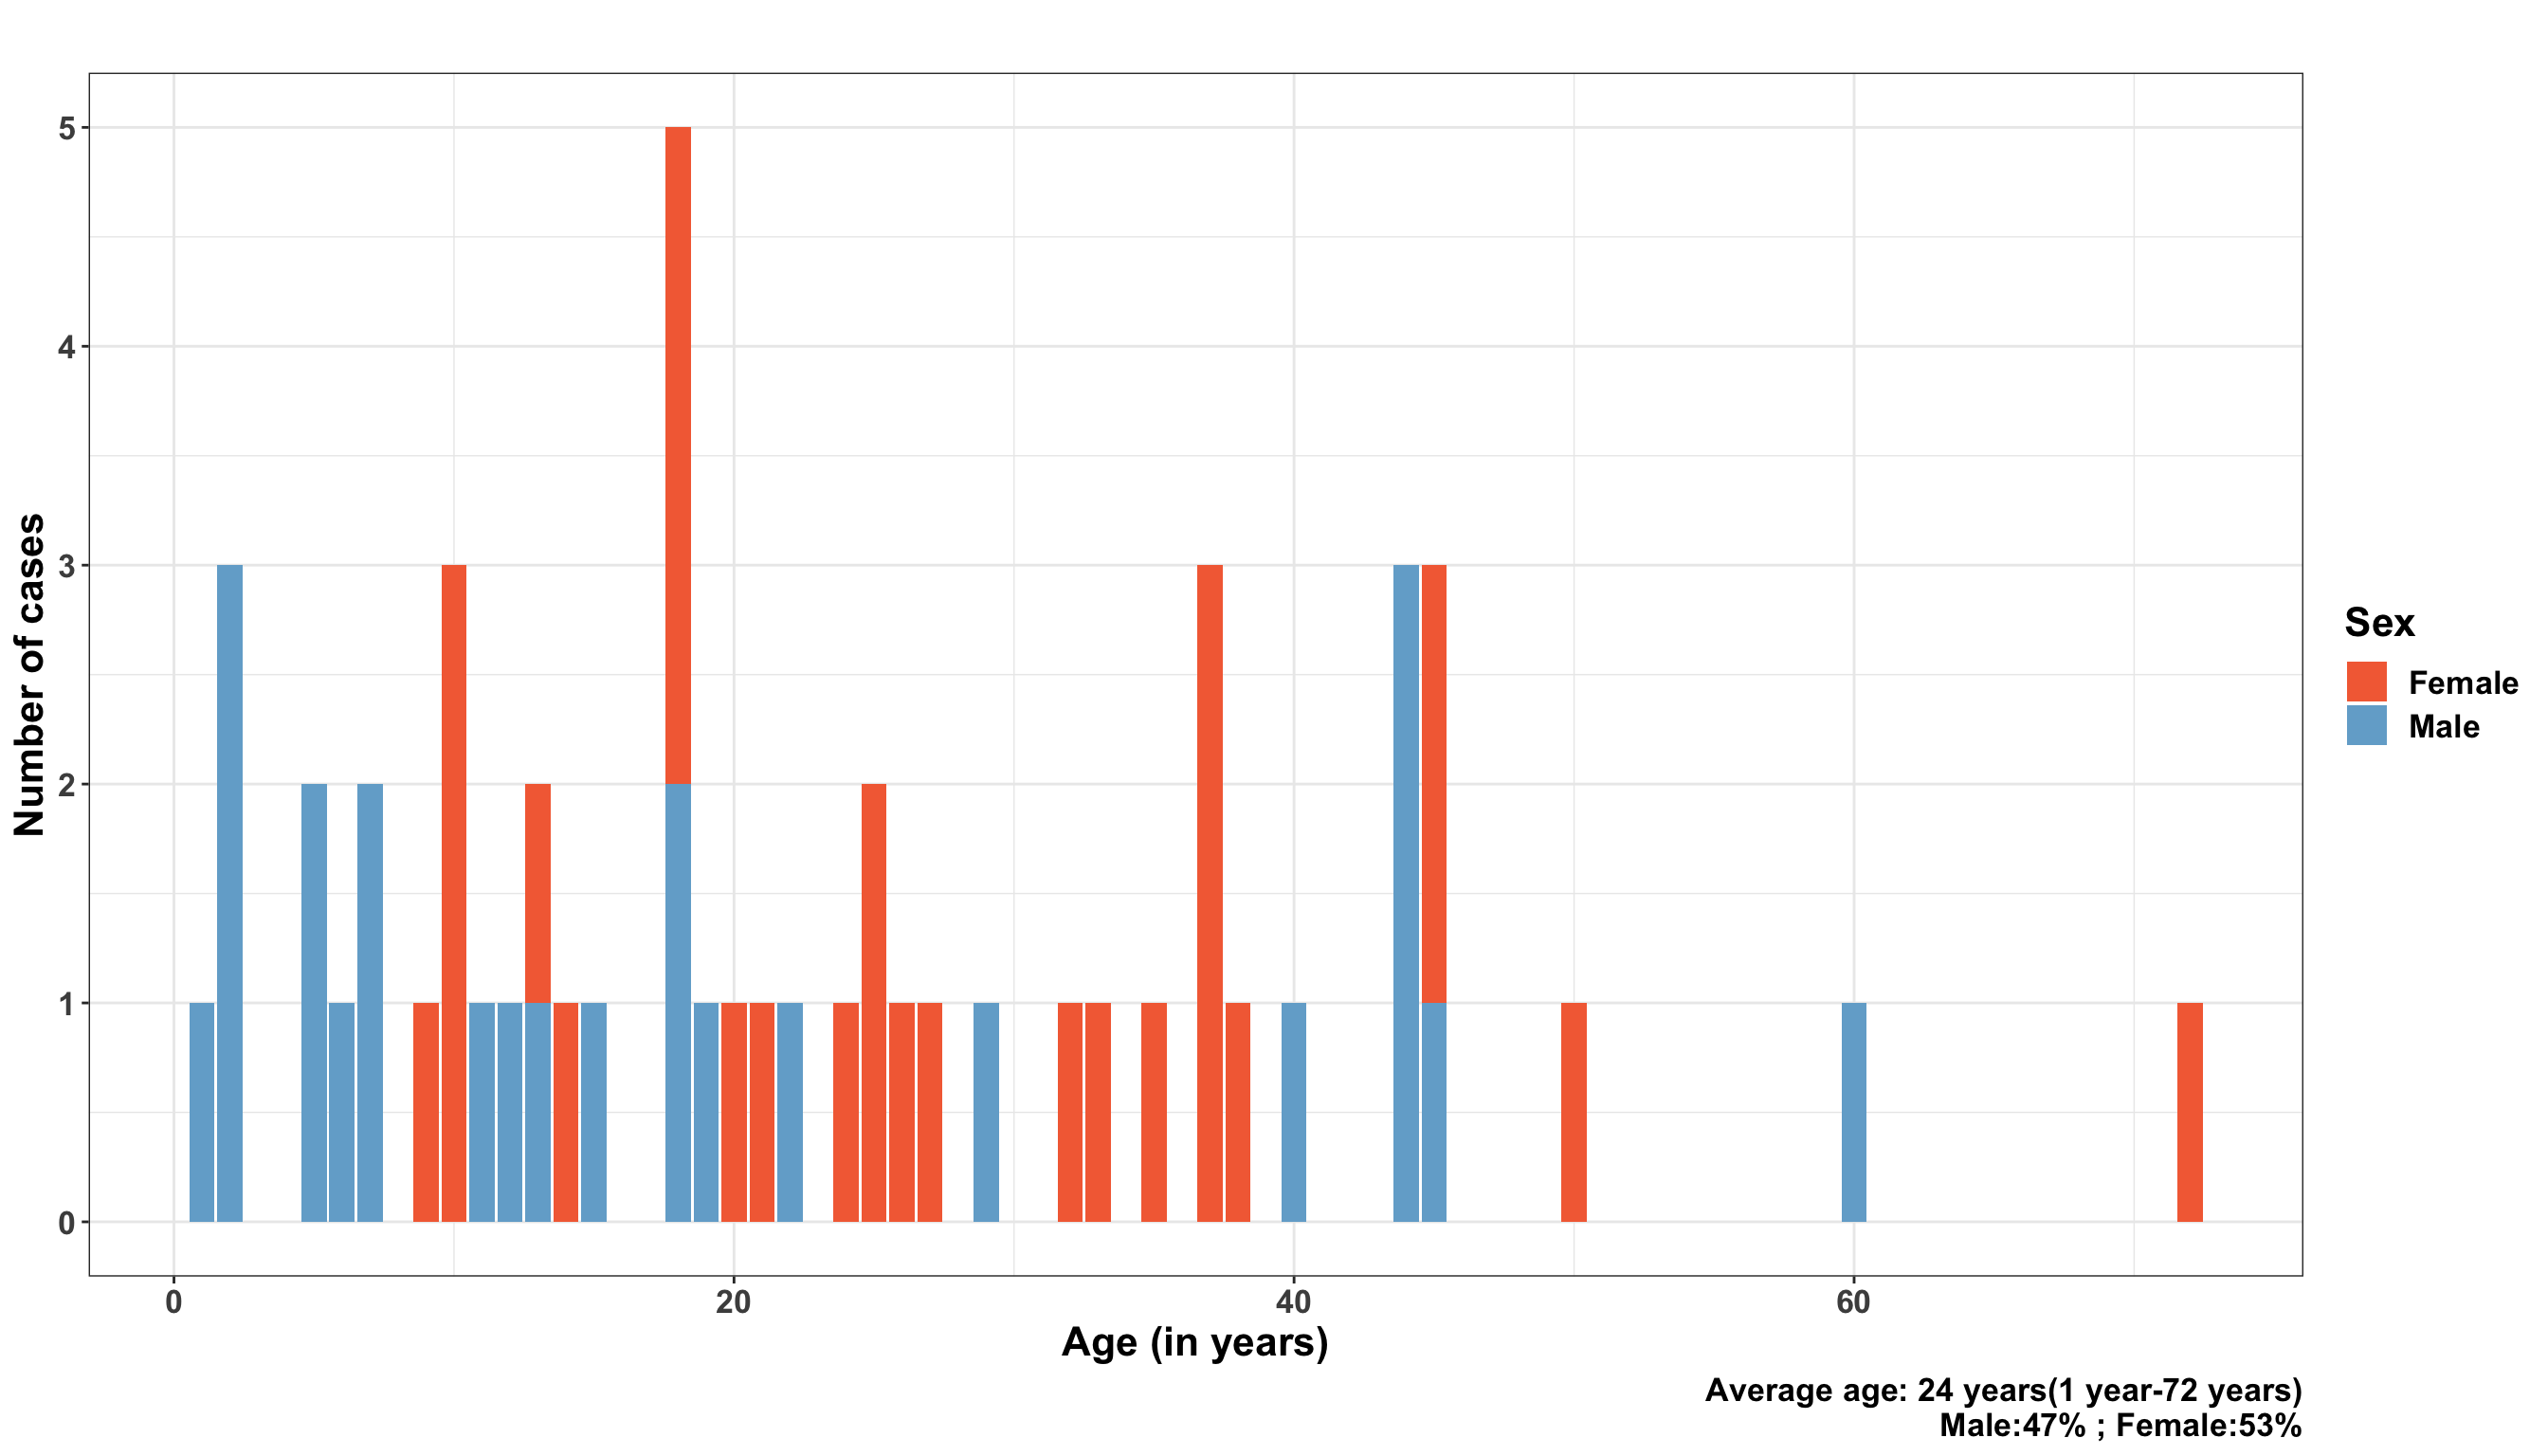
\includegraphics{_main_files/figure-latex/unnamed-chunk-24-1.pdf}

\hypertarget{spatial-distribution-3}{%
\section{Spatial distribution}\label{spatial-distribution-3}}

The spatial distribution of these cases at subcounty level is as shown:

\hypertarget{kajiado}{%
\chapter{Kajiado}\label{kajiado}}

\hypertarget{cases-over-time-4}{%
\section{Cases over time}\label{cases-over-time-4}}

As at 2023-03-23, there were 231 cases reported in Kajiado County.

This is shown in the graph below:

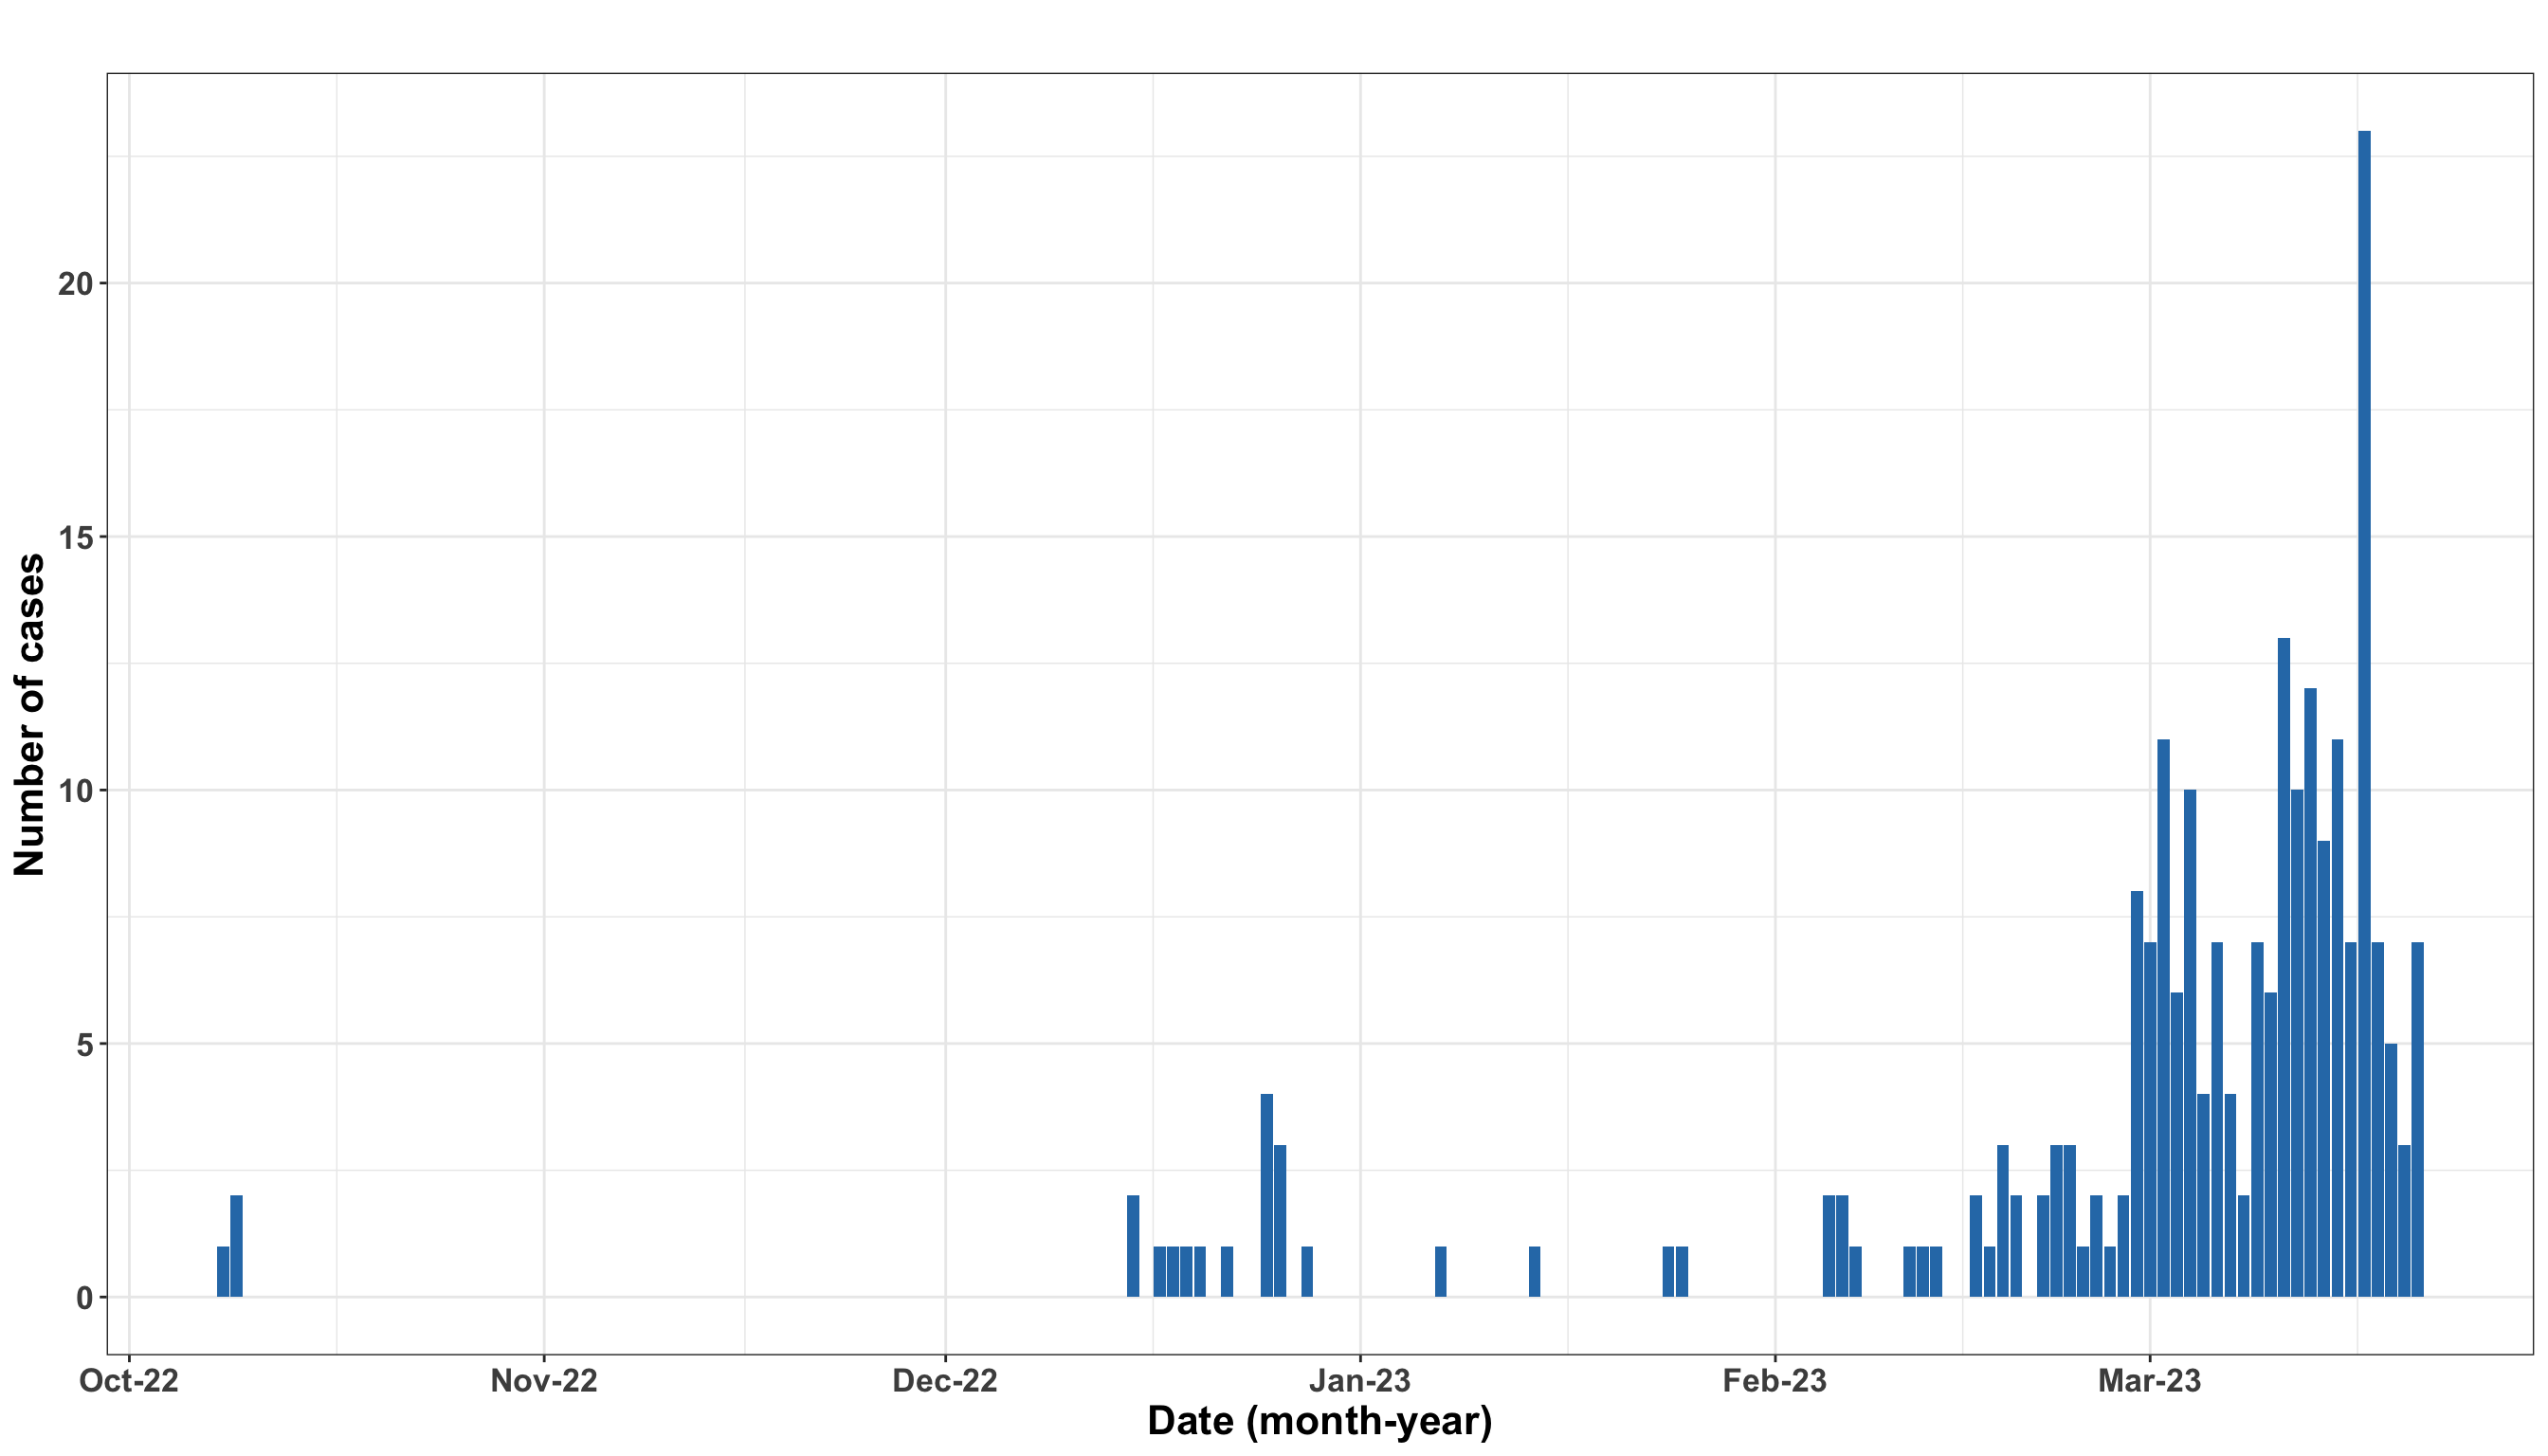
\includegraphics{_main_files/figure-latex/unnamed-chunk-28-1.pdf}

\hypertarget{demographic-distribution-4}{%
\section{Demographic distribution}\label{demographic-distribution-4}}

The stratification of these cases by age and sex is as shown:

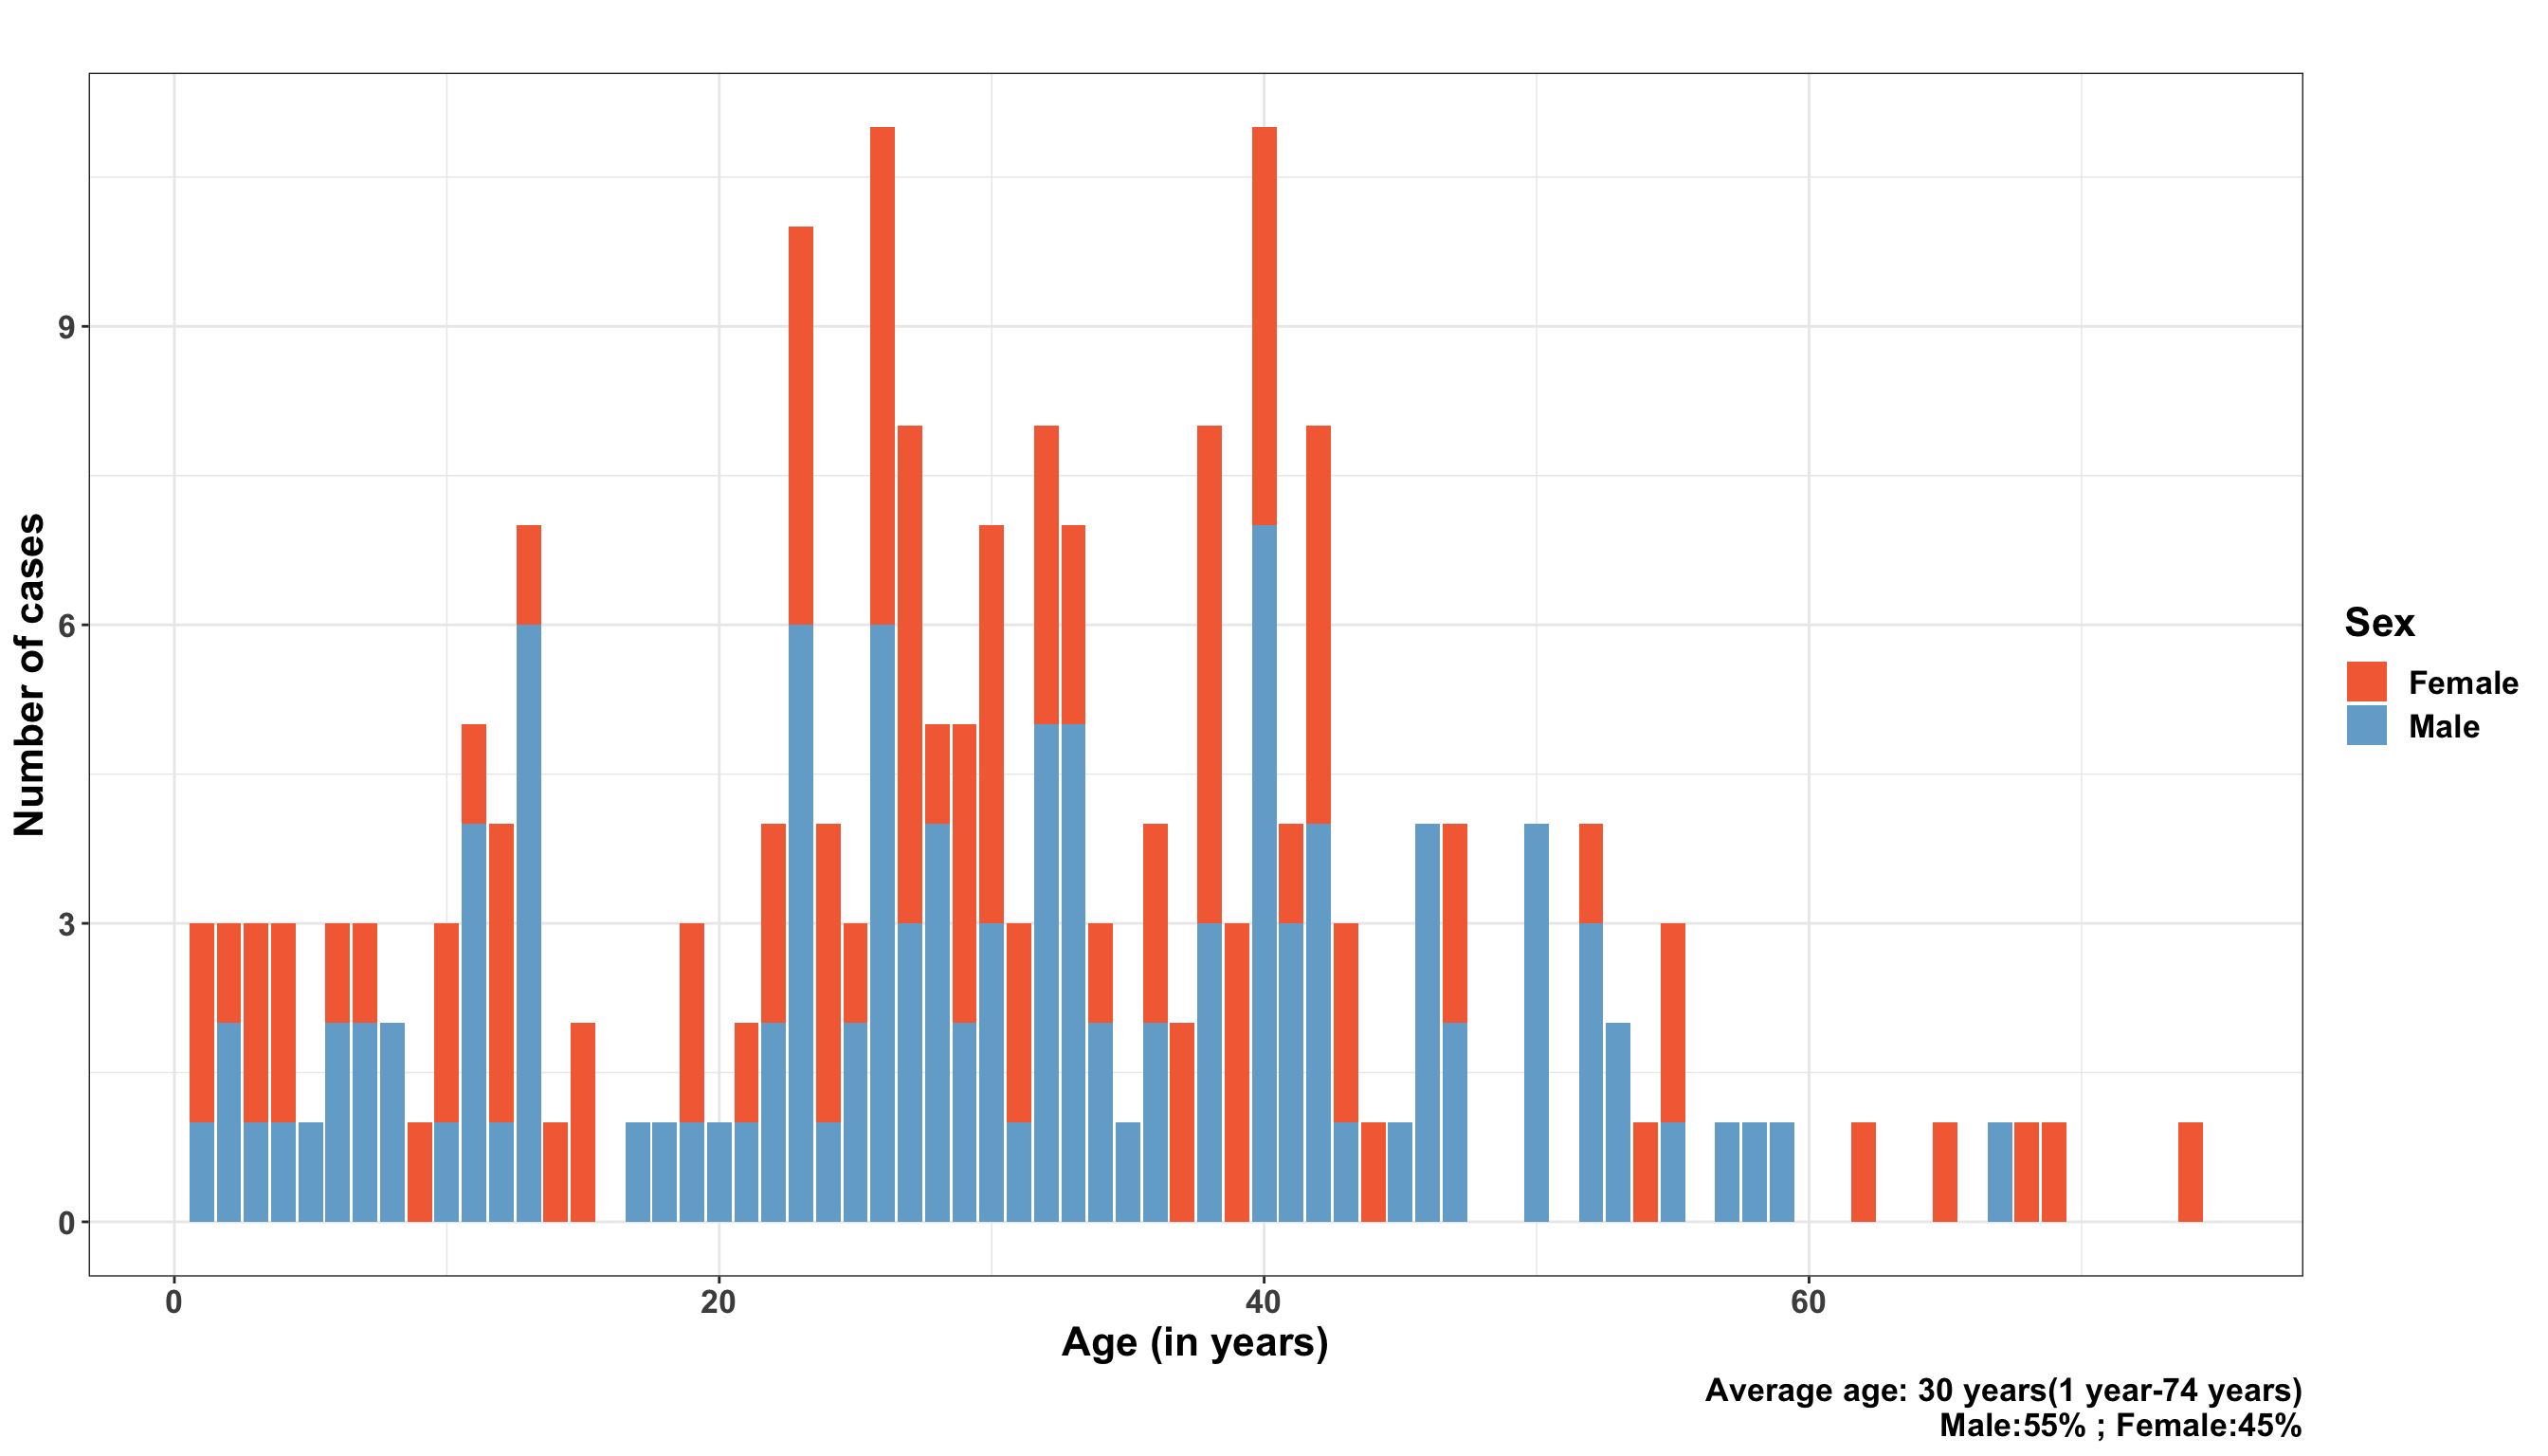
\includegraphics{_main_files/figure-latex/unnamed-chunk-30-1.pdf}

\hypertarget{spatial-distribution-4}{%
\section{Spatial distribution}\label{spatial-distribution-4}}

The spatial distribution of these cases at subcounty level is as shown:

\hypertarget{kiambu}{%
\chapter{Kiambu}\label{kiambu}}

\hypertarget{cases-over-time-5}{%
\section{Cases over time}\label{cases-over-time-5}}

As at 2023-03-23, there were 402 cases reported in Kiambu County.

This is shown in the graph below:

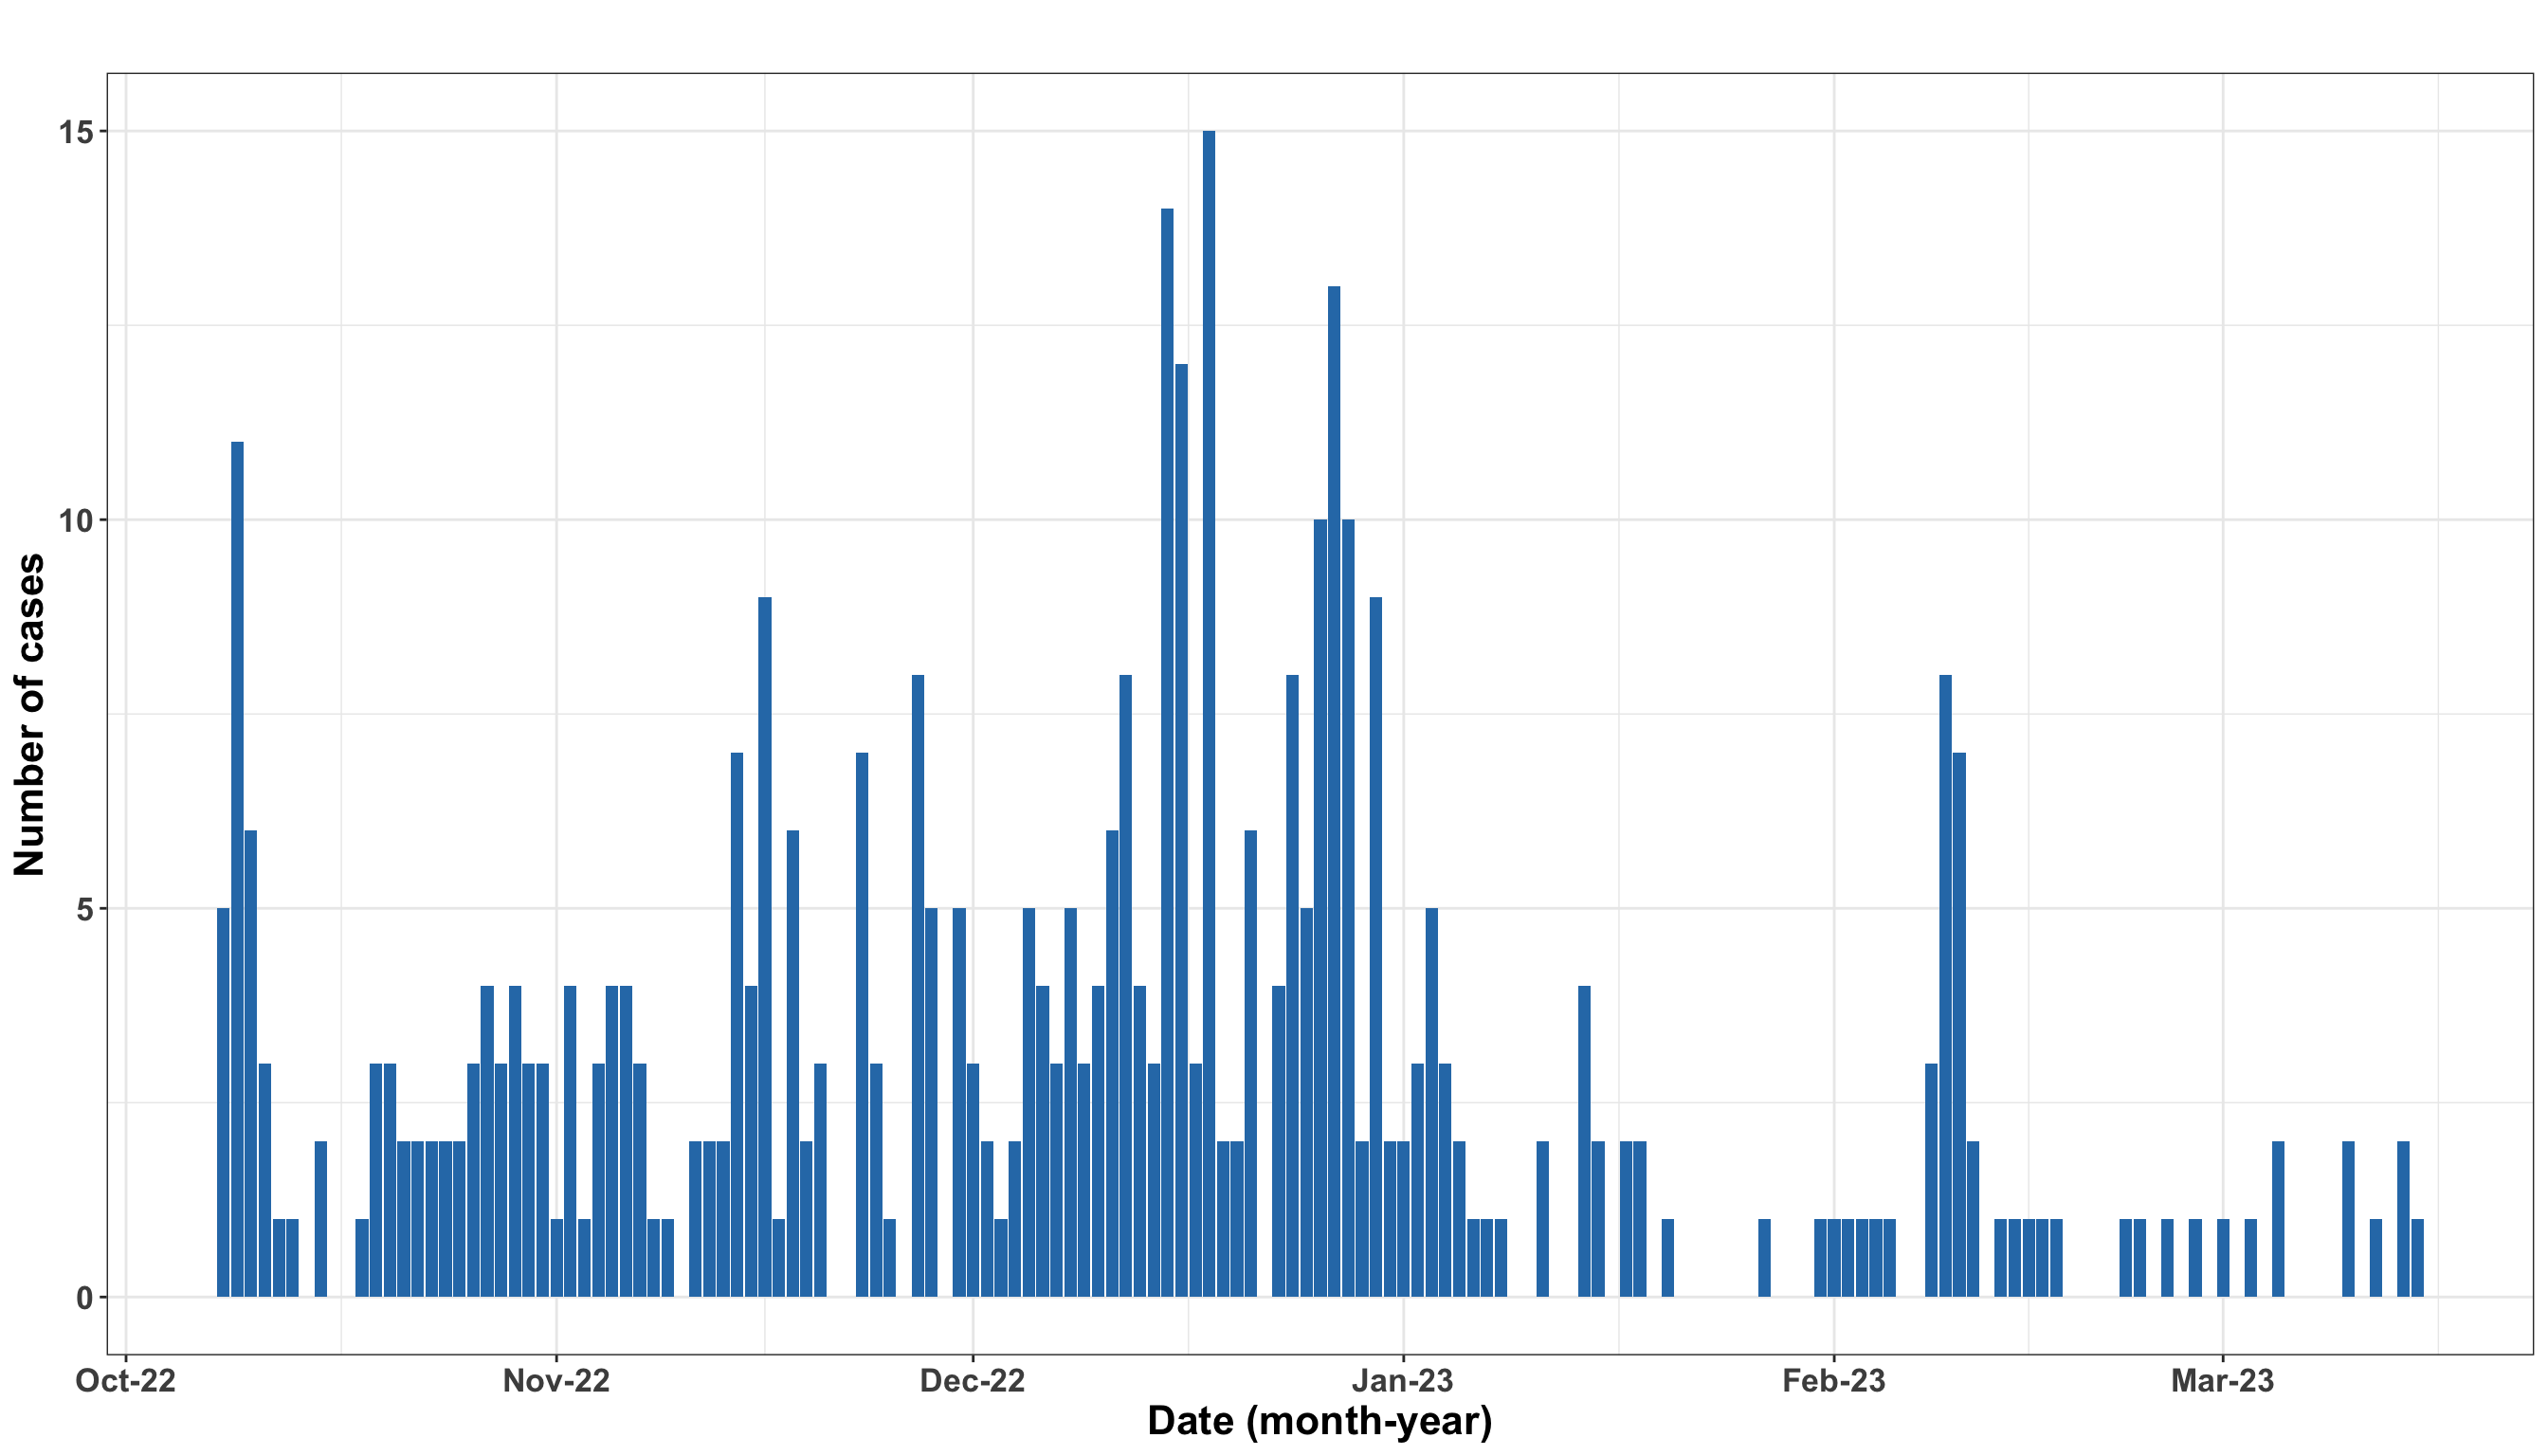
\includegraphics{_main_files/figure-latex/unnamed-chunk-34-1.pdf}

\hypertarget{demographic-distribution-5}{%
\section{Demographic distribution}\label{demographic-distribution-5}}

The stratification of these cases by age and sex is as shown:

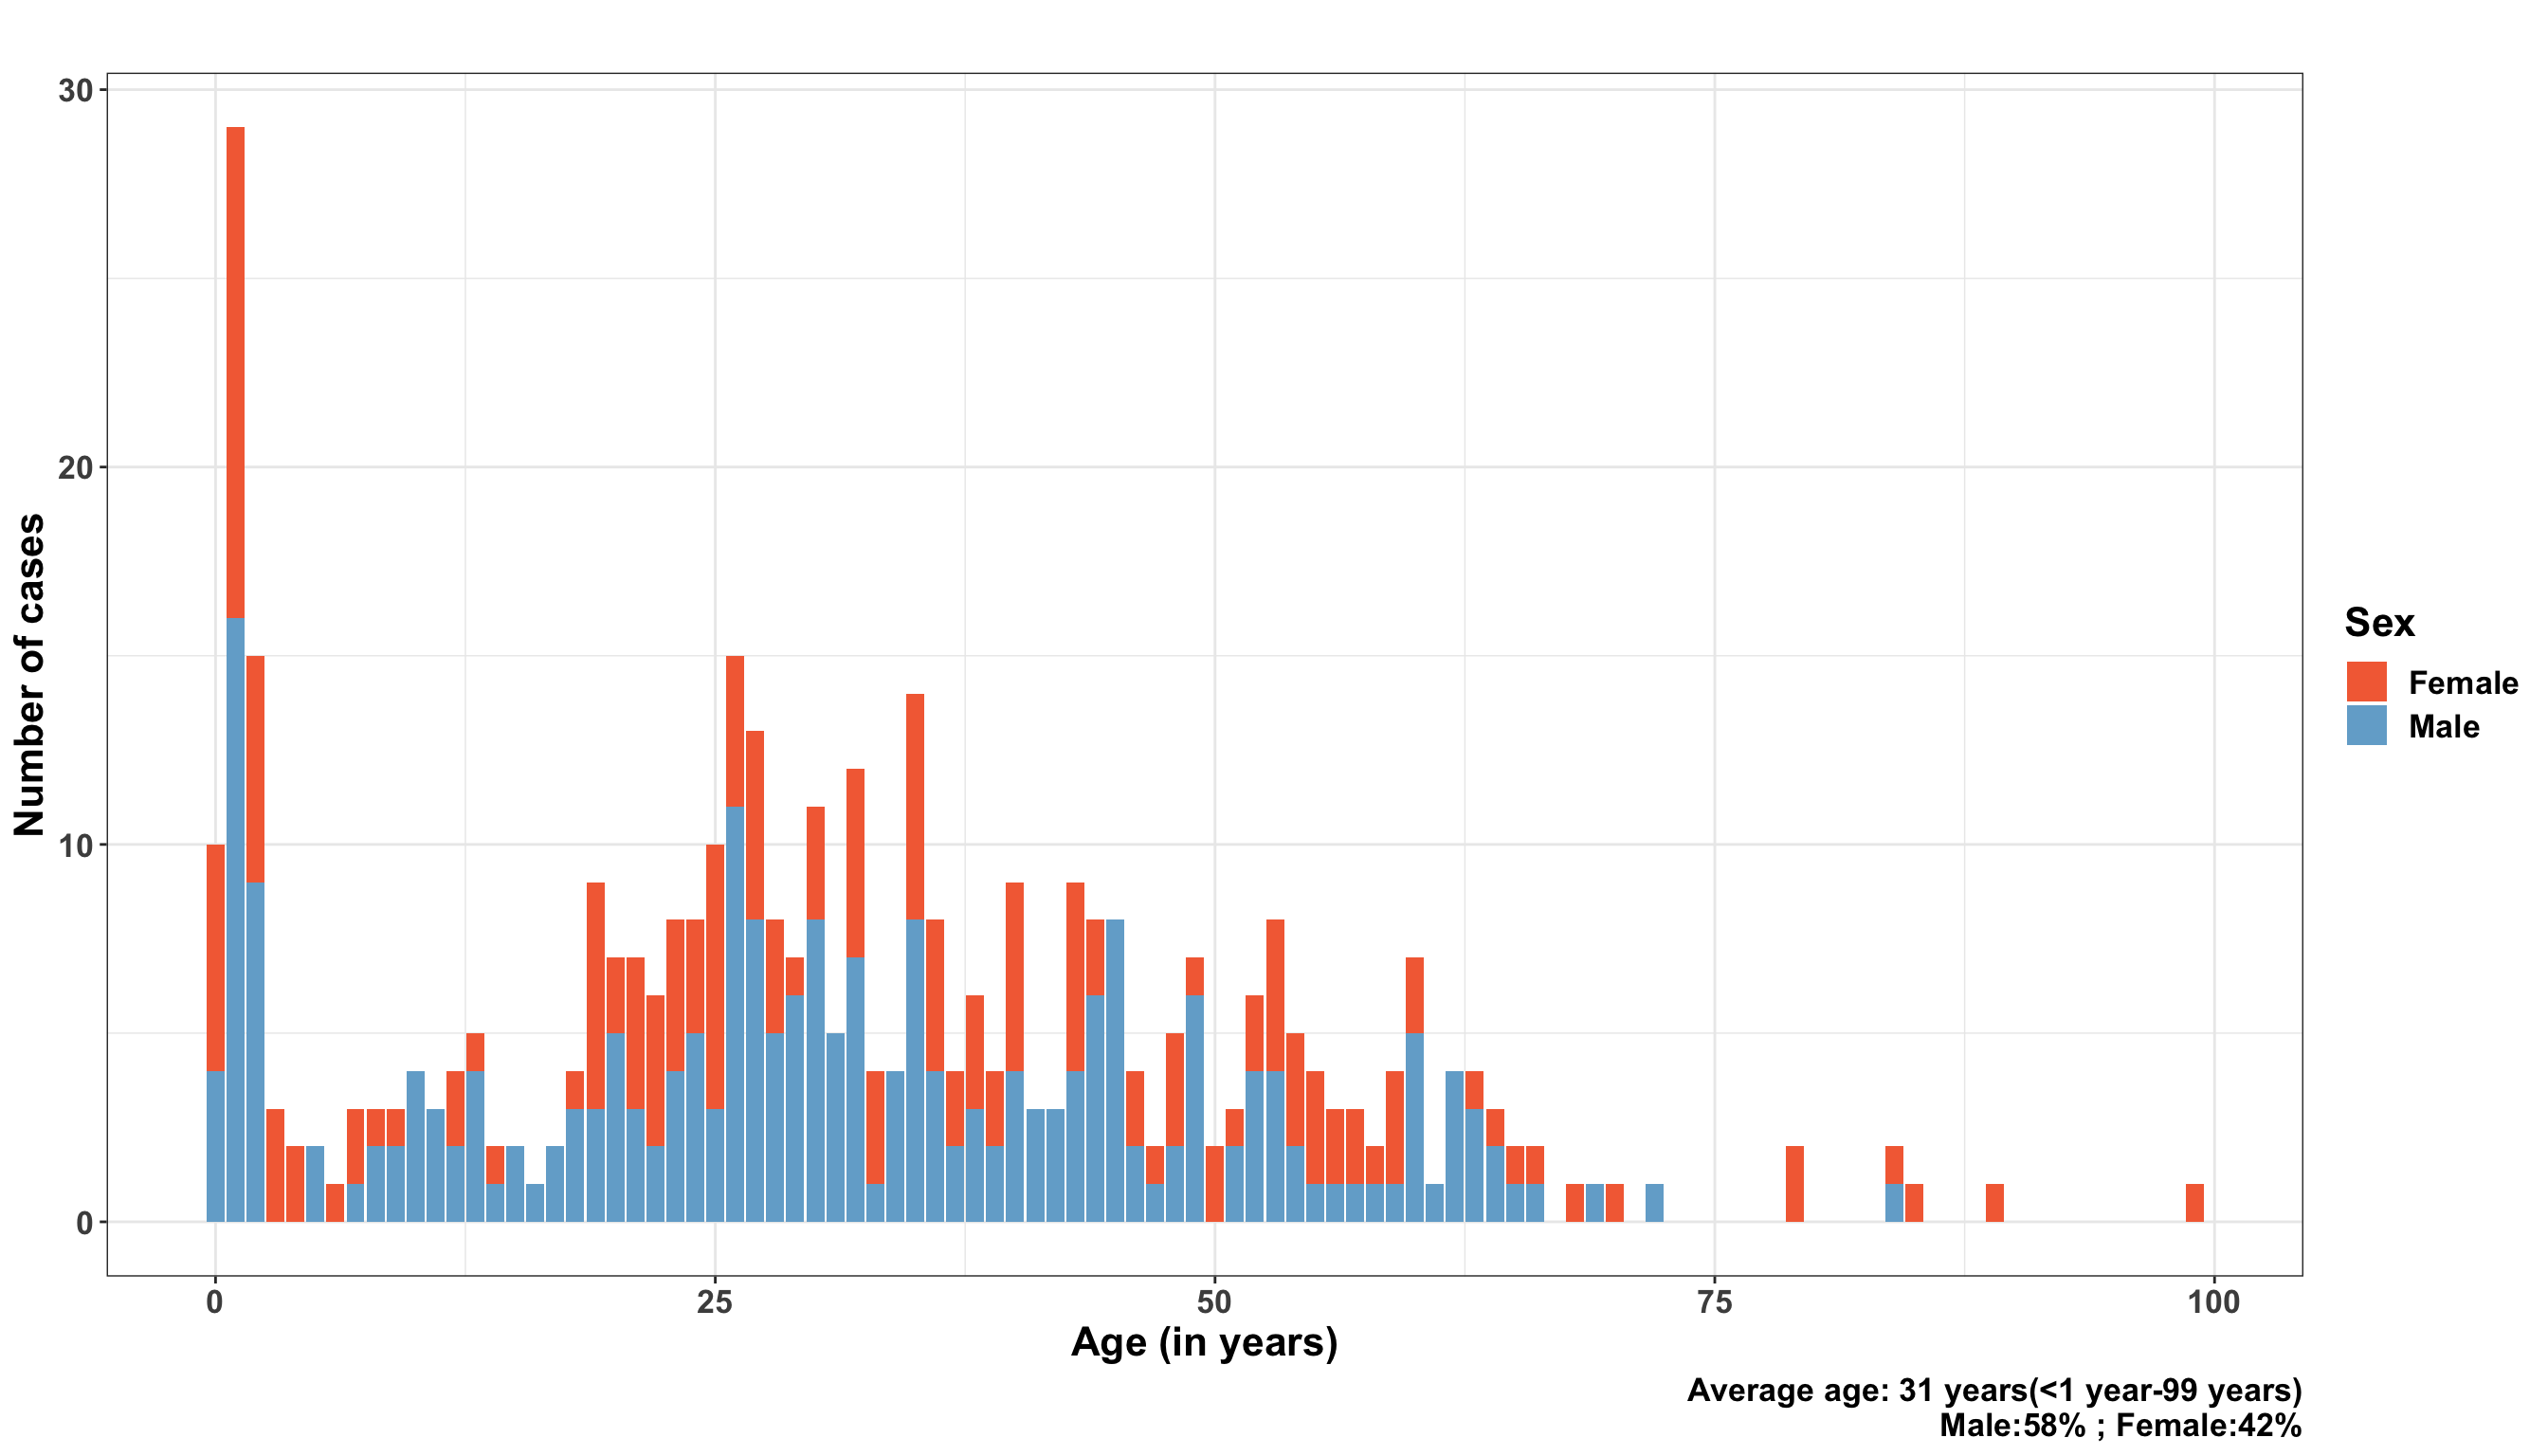
\includegraphics{_main_files/figure-latex/unnamed-chunk-36-1.pdf}

\hypertarget{spatial-distribution-5}{%
\section{Spatial distribution}\label{spatial-distribution-5}}

The spatial distribution of these cases at subcounty level is as shown:

\hypertarget{kitui}{%
\chapter{Kitui}\label{kitui}}

\hypertarget{cases-over-time-6}{%
\section{Cases over time}\label{cases-over-time-6}}

As at 2023-03-23, there were 26 cases reported in Kitui County.

This is shown in the graph below:

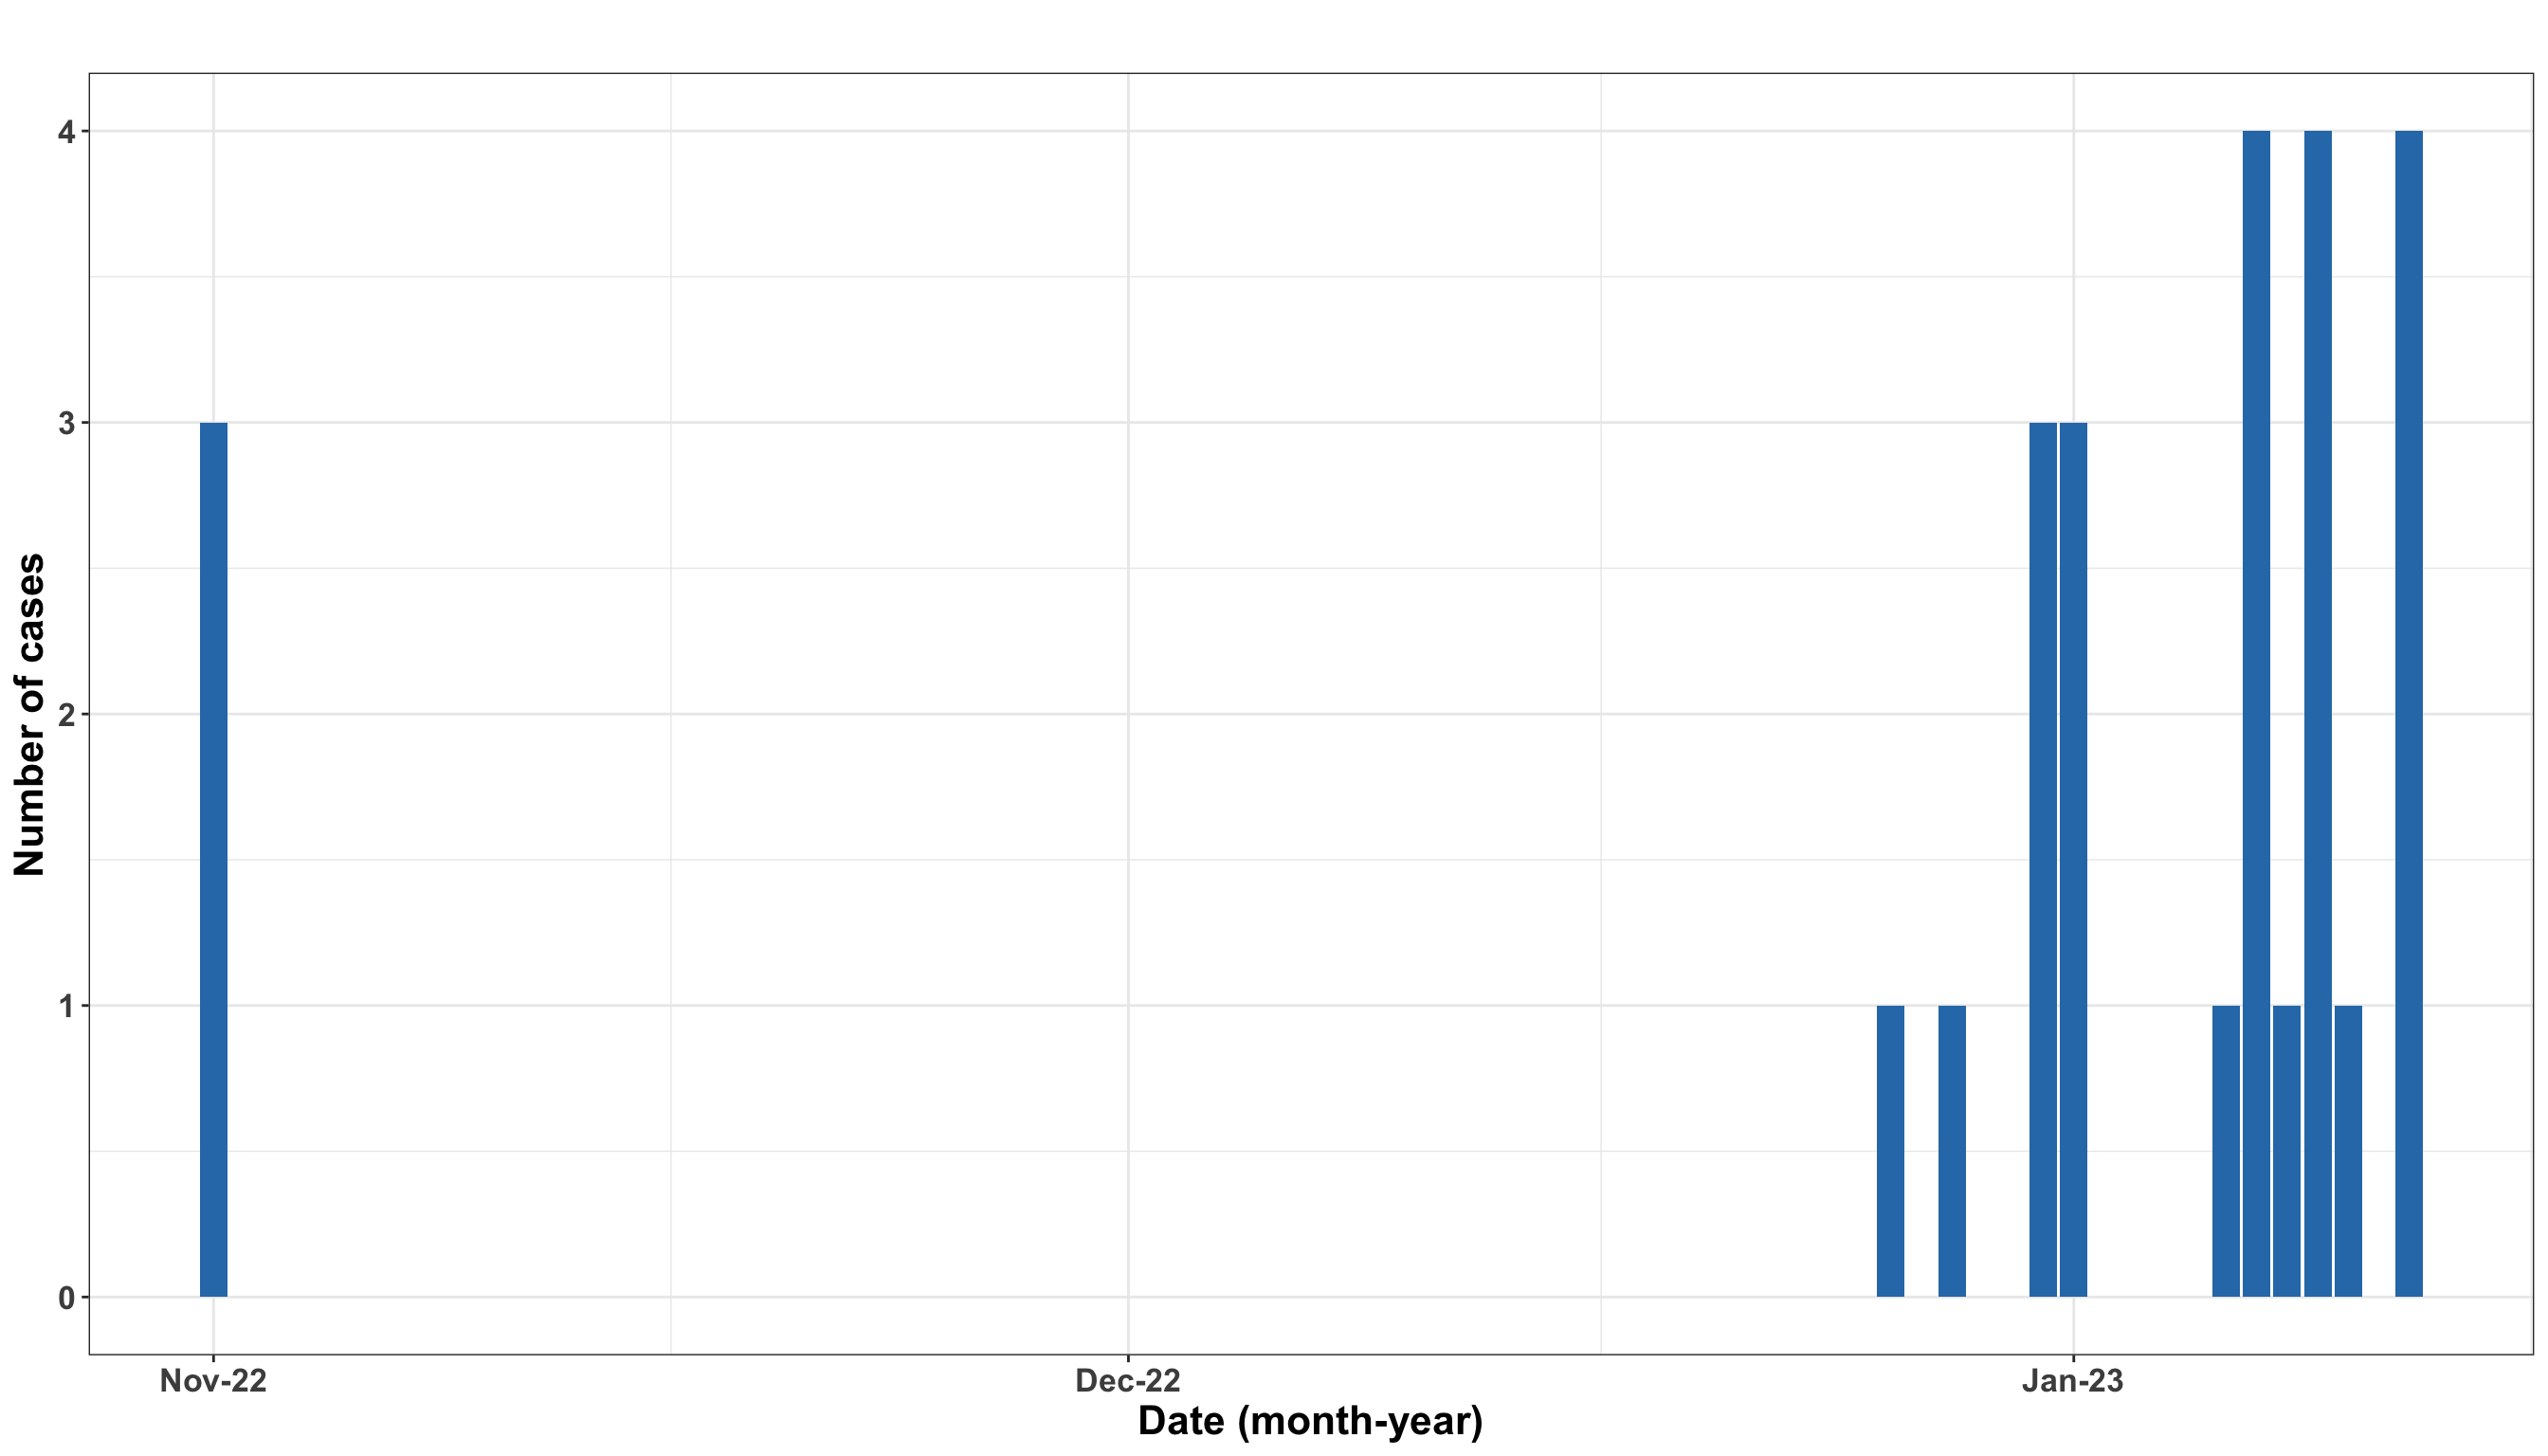
\includegraphics{_main_files/figure-latex/unnamed-chunk-40-1.pdf}

\hypertarget{demographic-distribution-6}{%
\section{Demographic distribution}\label{demographic-distribution-6}}

The stratification of these cases by age and sex is as shown:

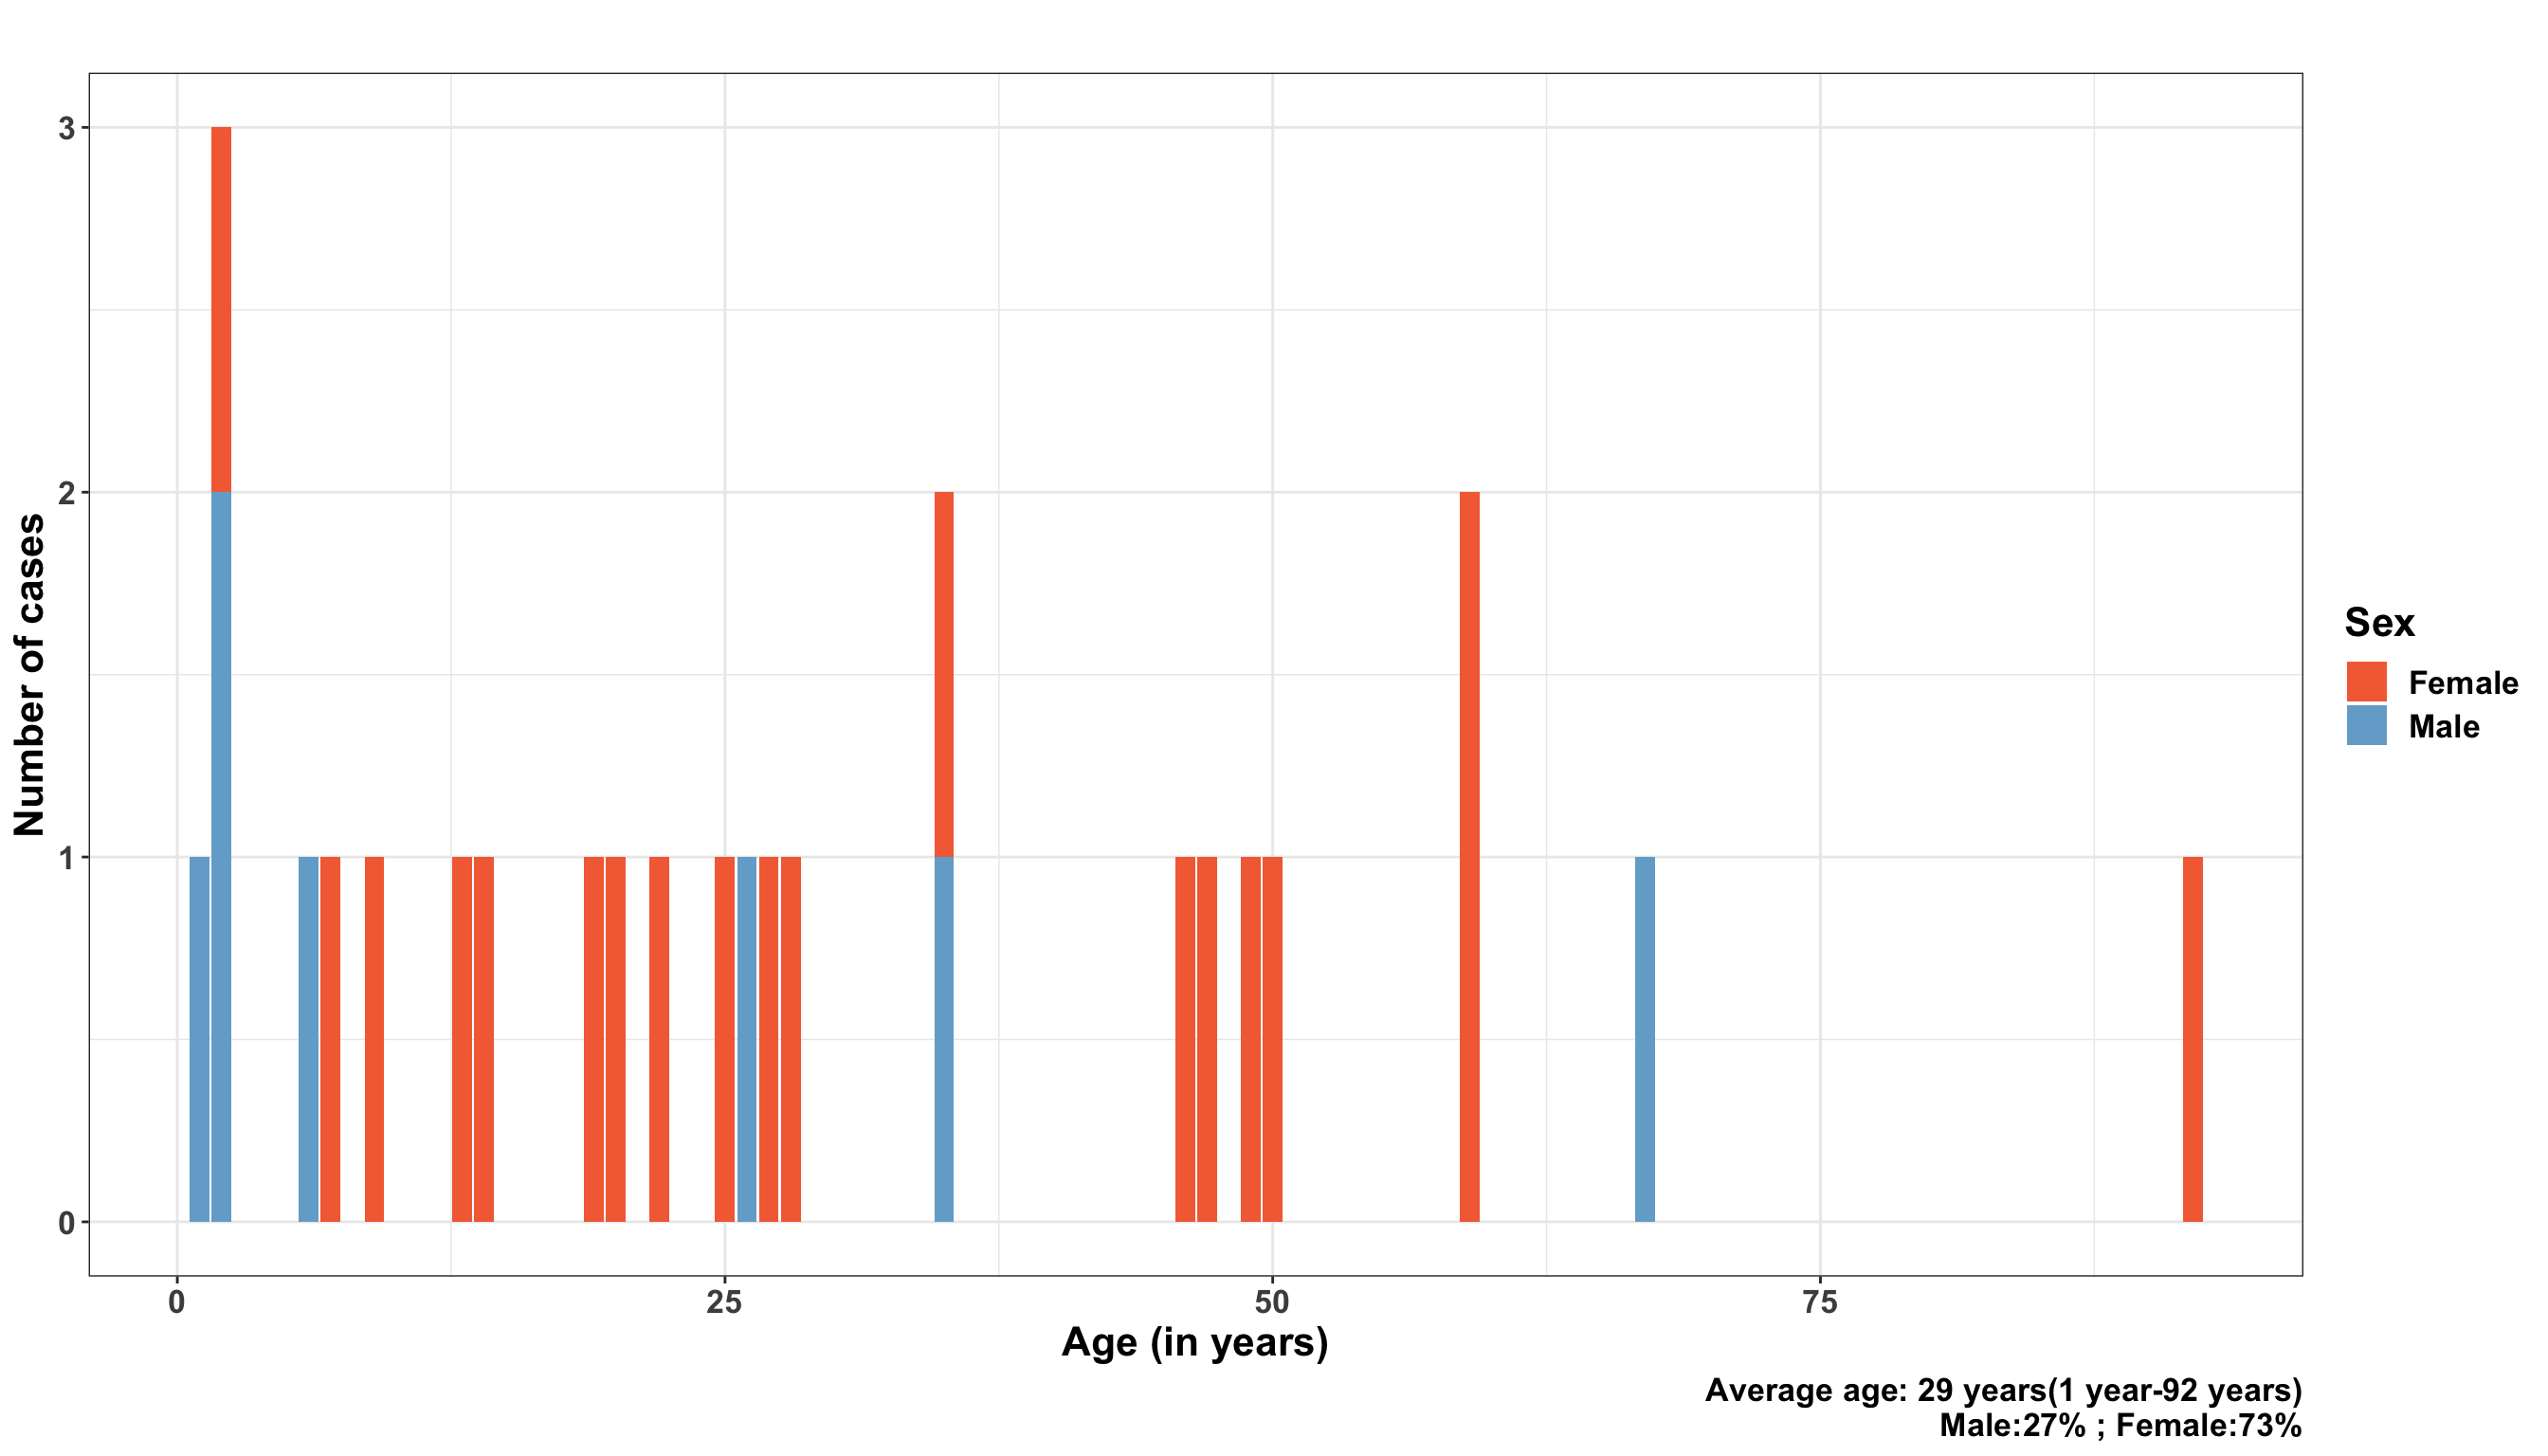
\includegraphics{_main_files/figure-latex/unnamed-chunk-42-1.pdf}

\hypertarget{spatial-distribution-6}{%
\section{Spatial distribution}\label{spatial-distribution-6}}

The spatial distribution of these cases at subcounty level is as shown:

\hypertarget{machakos}{%
\chapter{Machakos}\label{machakos}}

\hypertarget{cases-over-time-7}{%
\section{Cases over time}\label{cases-over-time-7}}

As at 2023-03-23, there were 352 cases reported in Machakos County.

This is shown in the graph below:

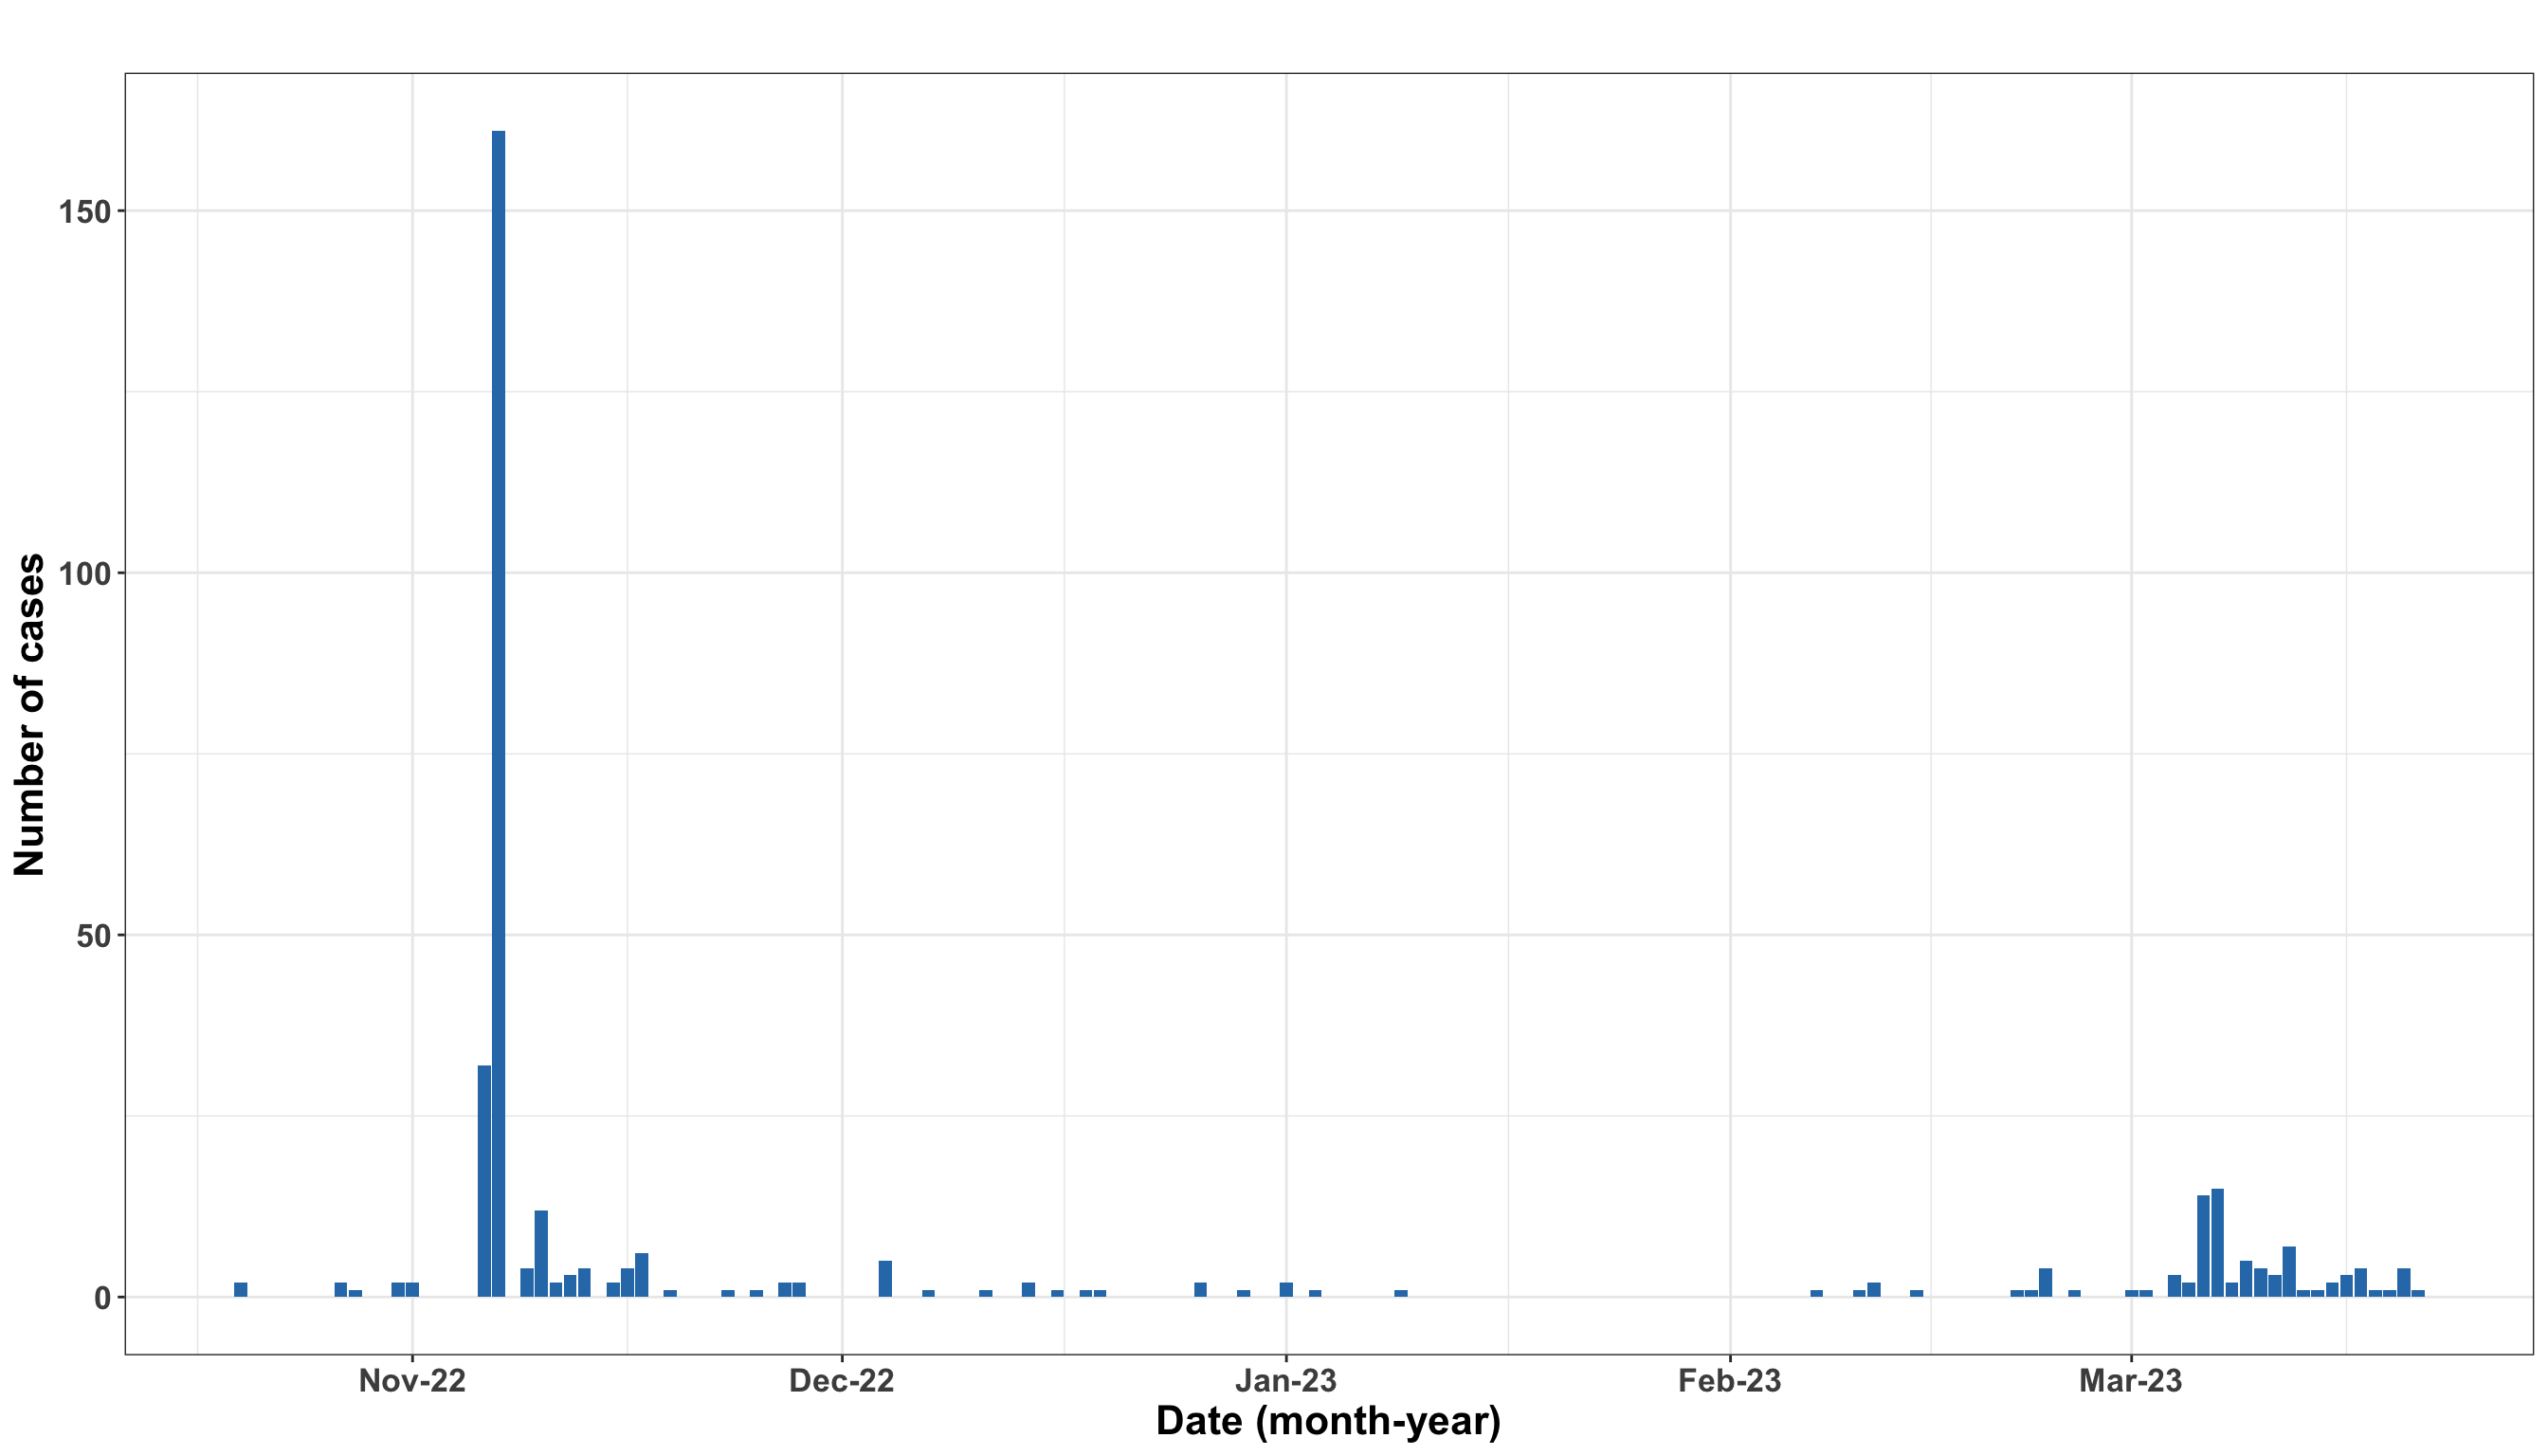
\includegraphics{_main_files/figure-latex/unnamed-chunk-46-1.pdf}

\hypertarget{demographic-distribution-7}{%
\section{Demographic distribution}\label{demographic-distribution-7}}

The stratification of these cases by age and sex is as shown:

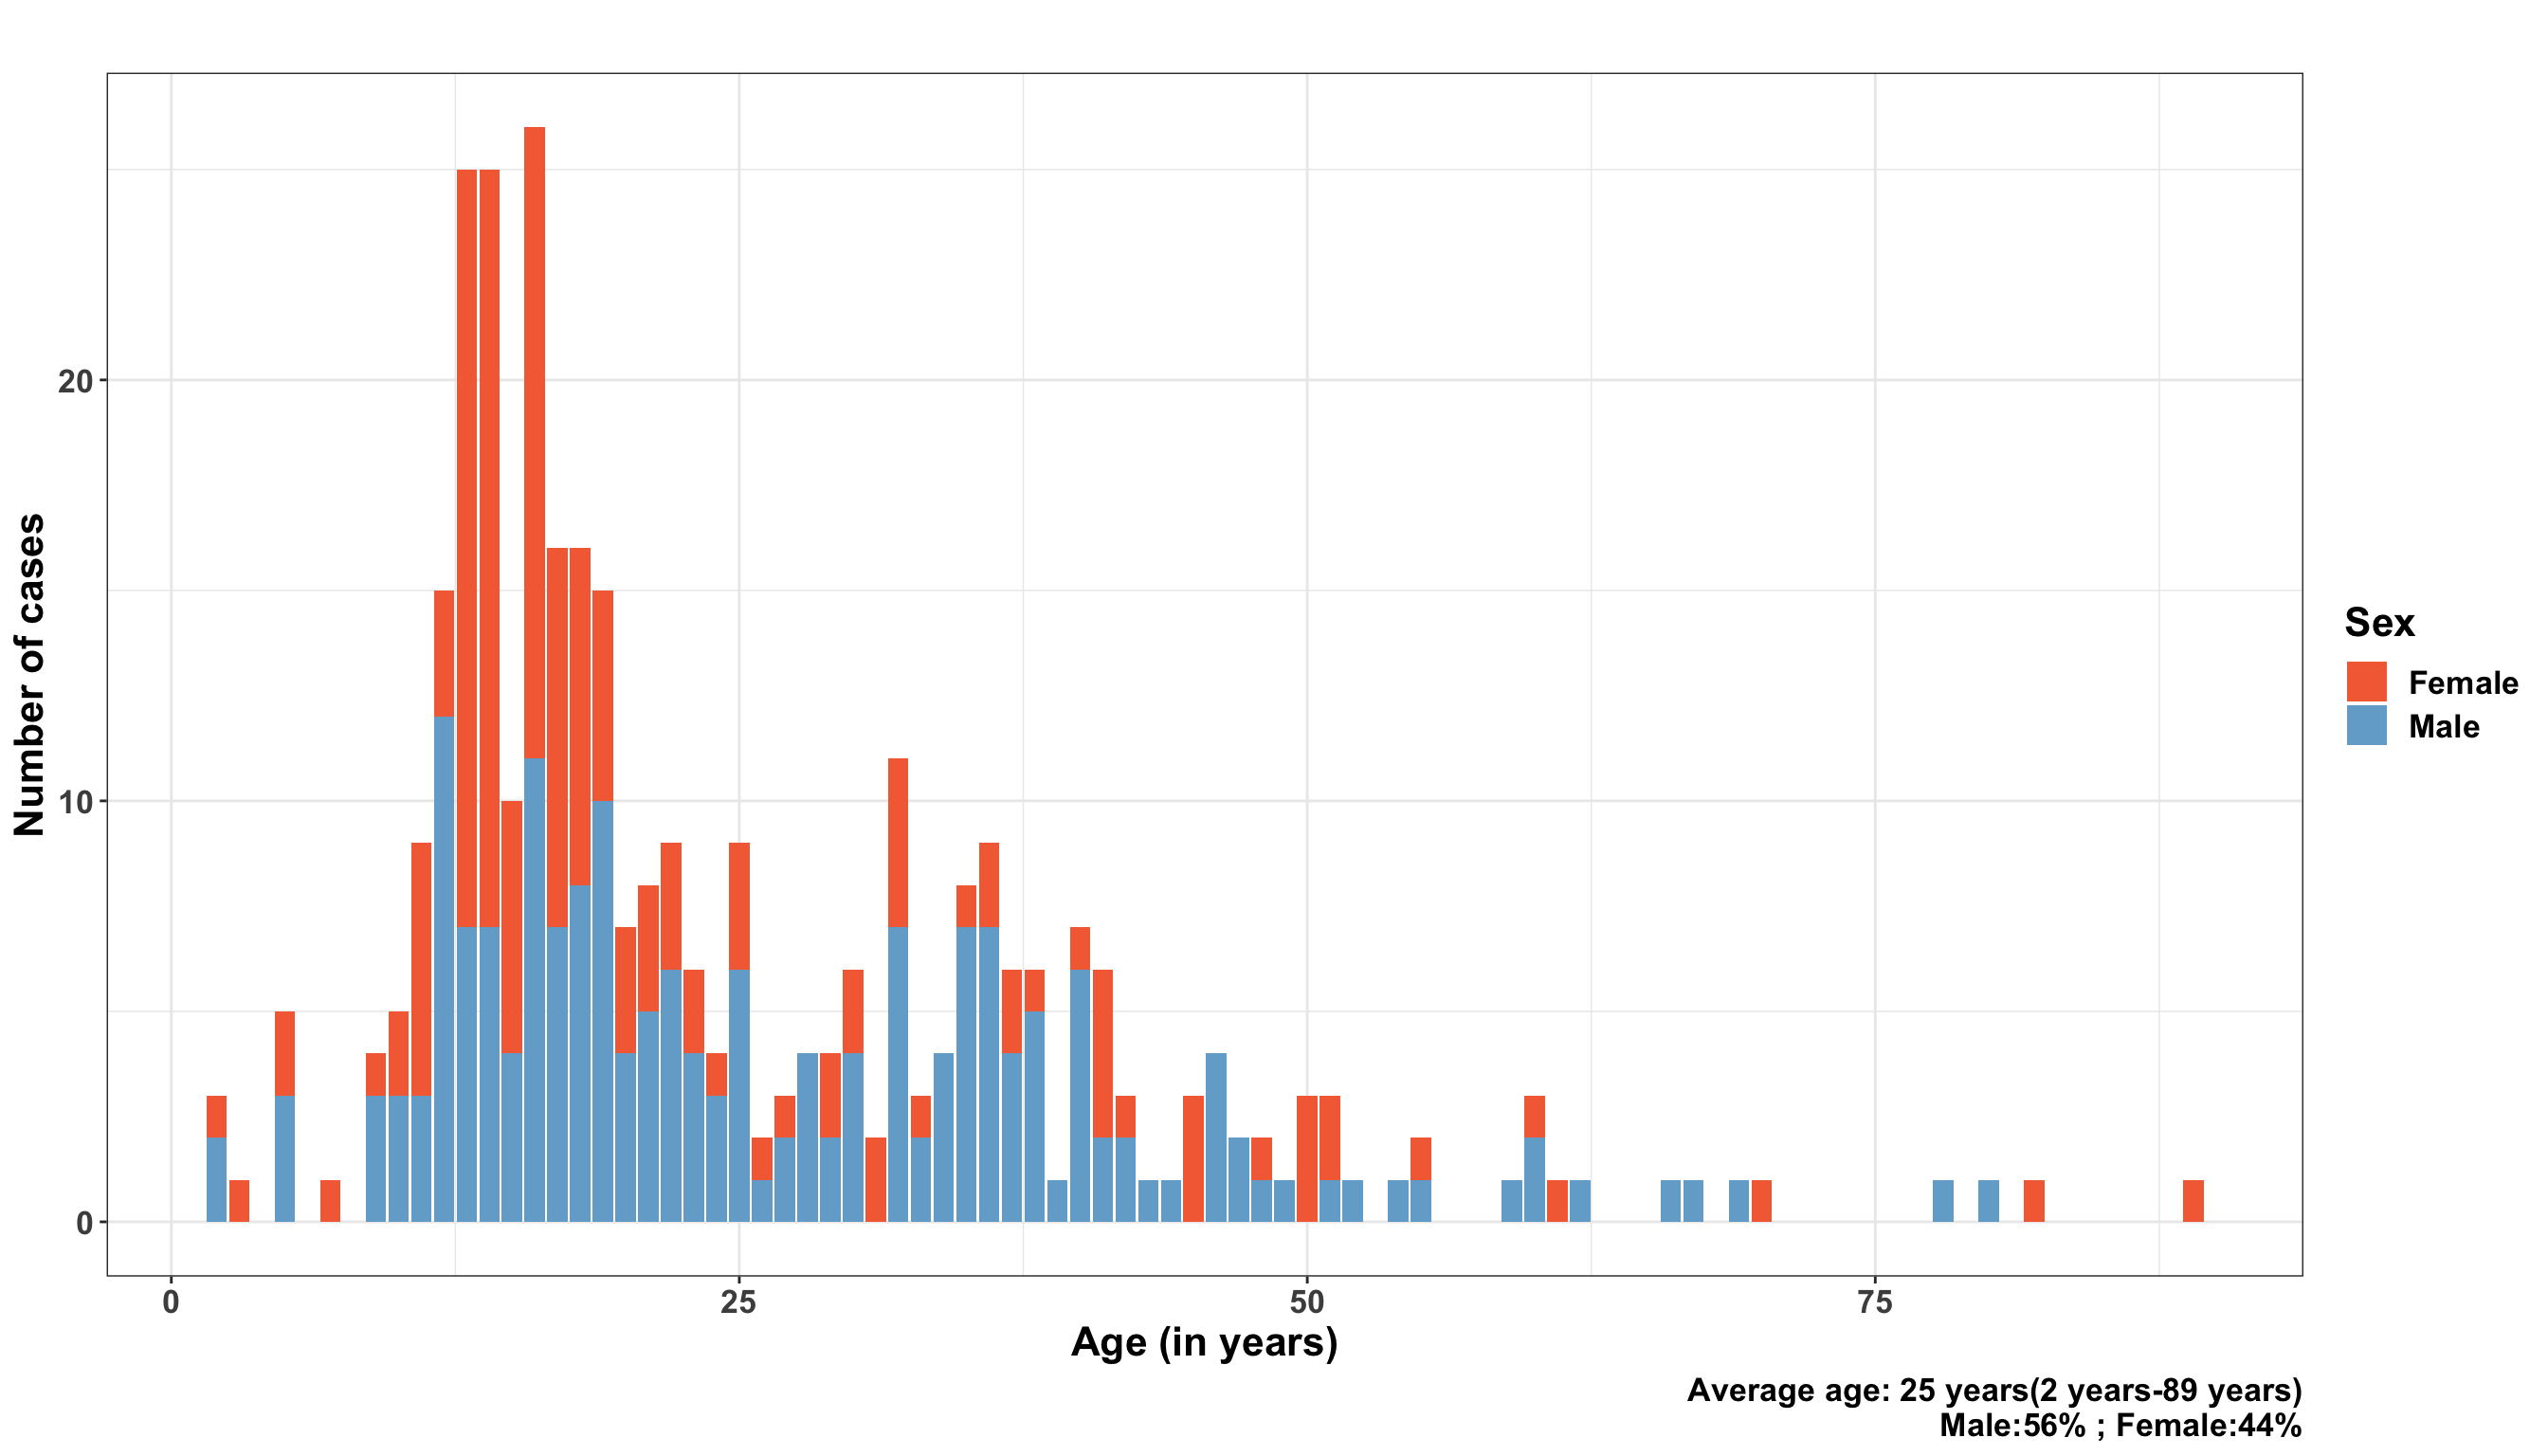
\includegraphics{_main_files/figure-latex/unnamed-chunk-48-1.pdf}

\hypertarget{spatial-distribution-7}{%
\section{Spatial distribution}\label{spatial-distribution-7}}

The spatial distribution of these cases at subcounty level is as shown:

\hypertarget{mandera}{%
\chapter{Mandera}\label{mandera}}

\hypertarget{cases-over-time-8}{%
\section{Cases over time}\label{cases-over-time-8}}

As at 2023-03-23, there were 1464 cases reported in Mandera County.

This is shown in the graph below:

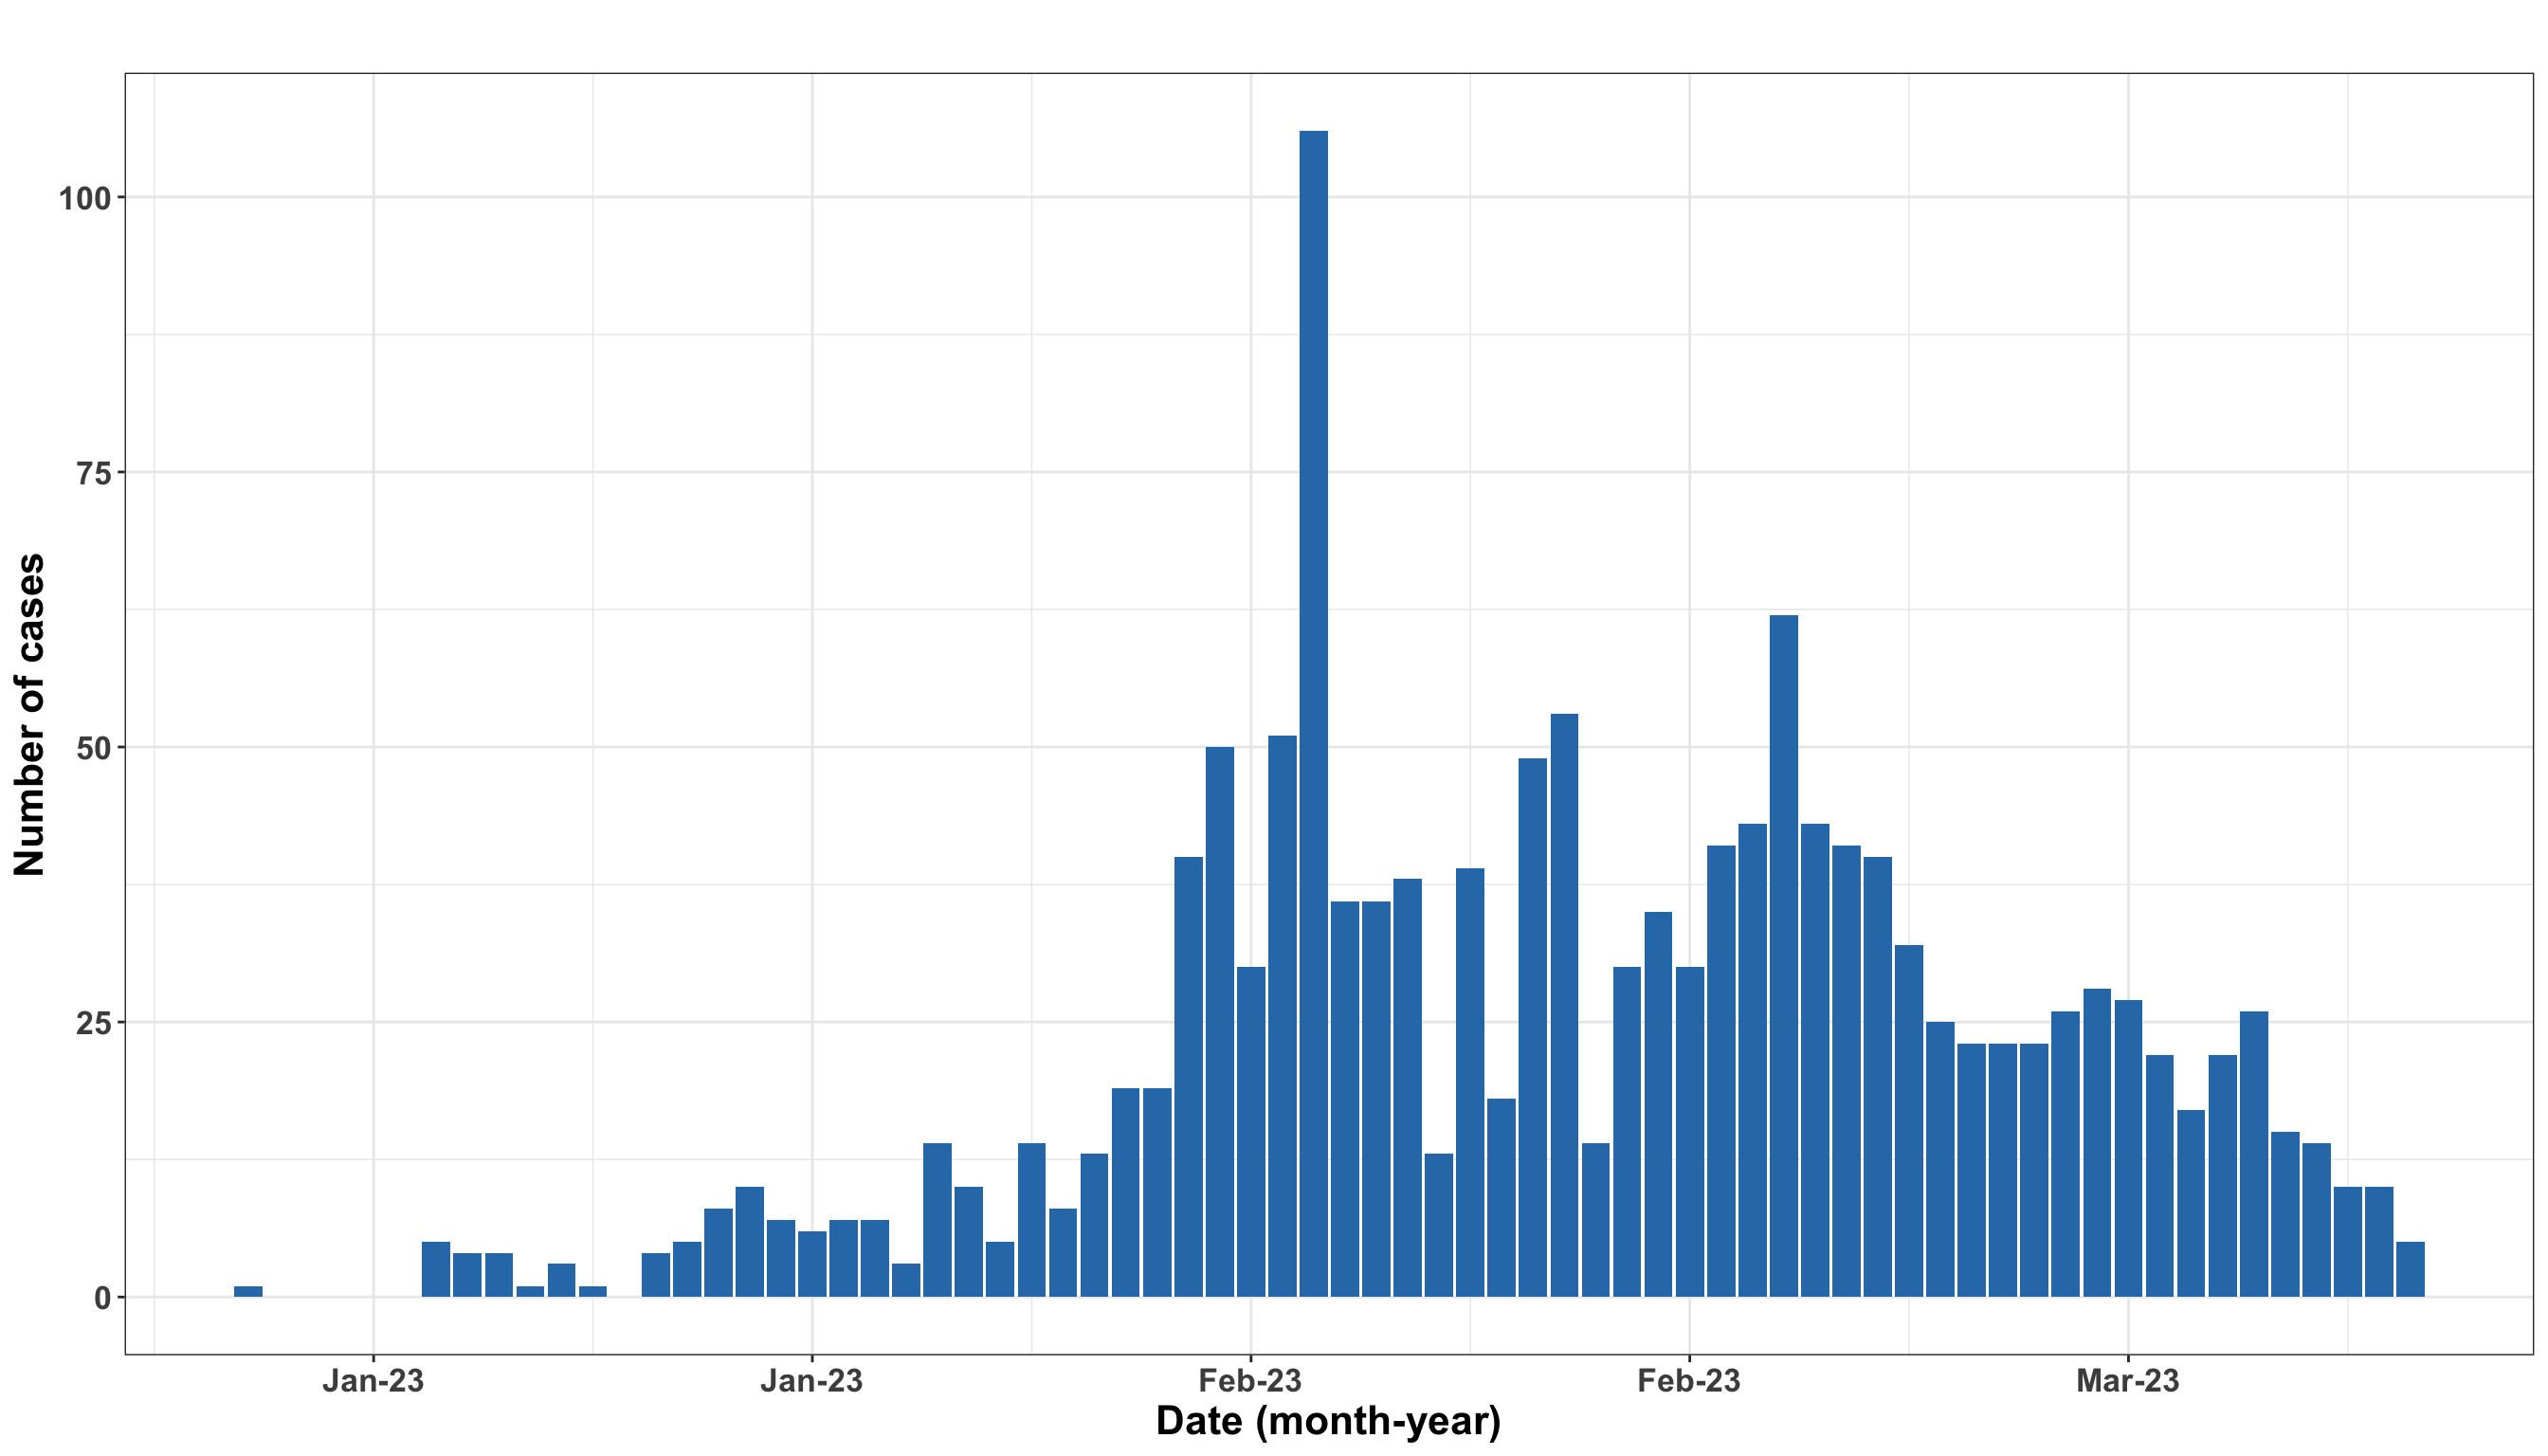
\includegraphics{_main_files/figure-latex/unnamed-chunk-52-1.pdf}

\hypertarget{demographic-distribution-8}{%
\section{Demographic distribution}\label{demographic-distribution-8}}

The stratification of these cases by age and sex is as shown:

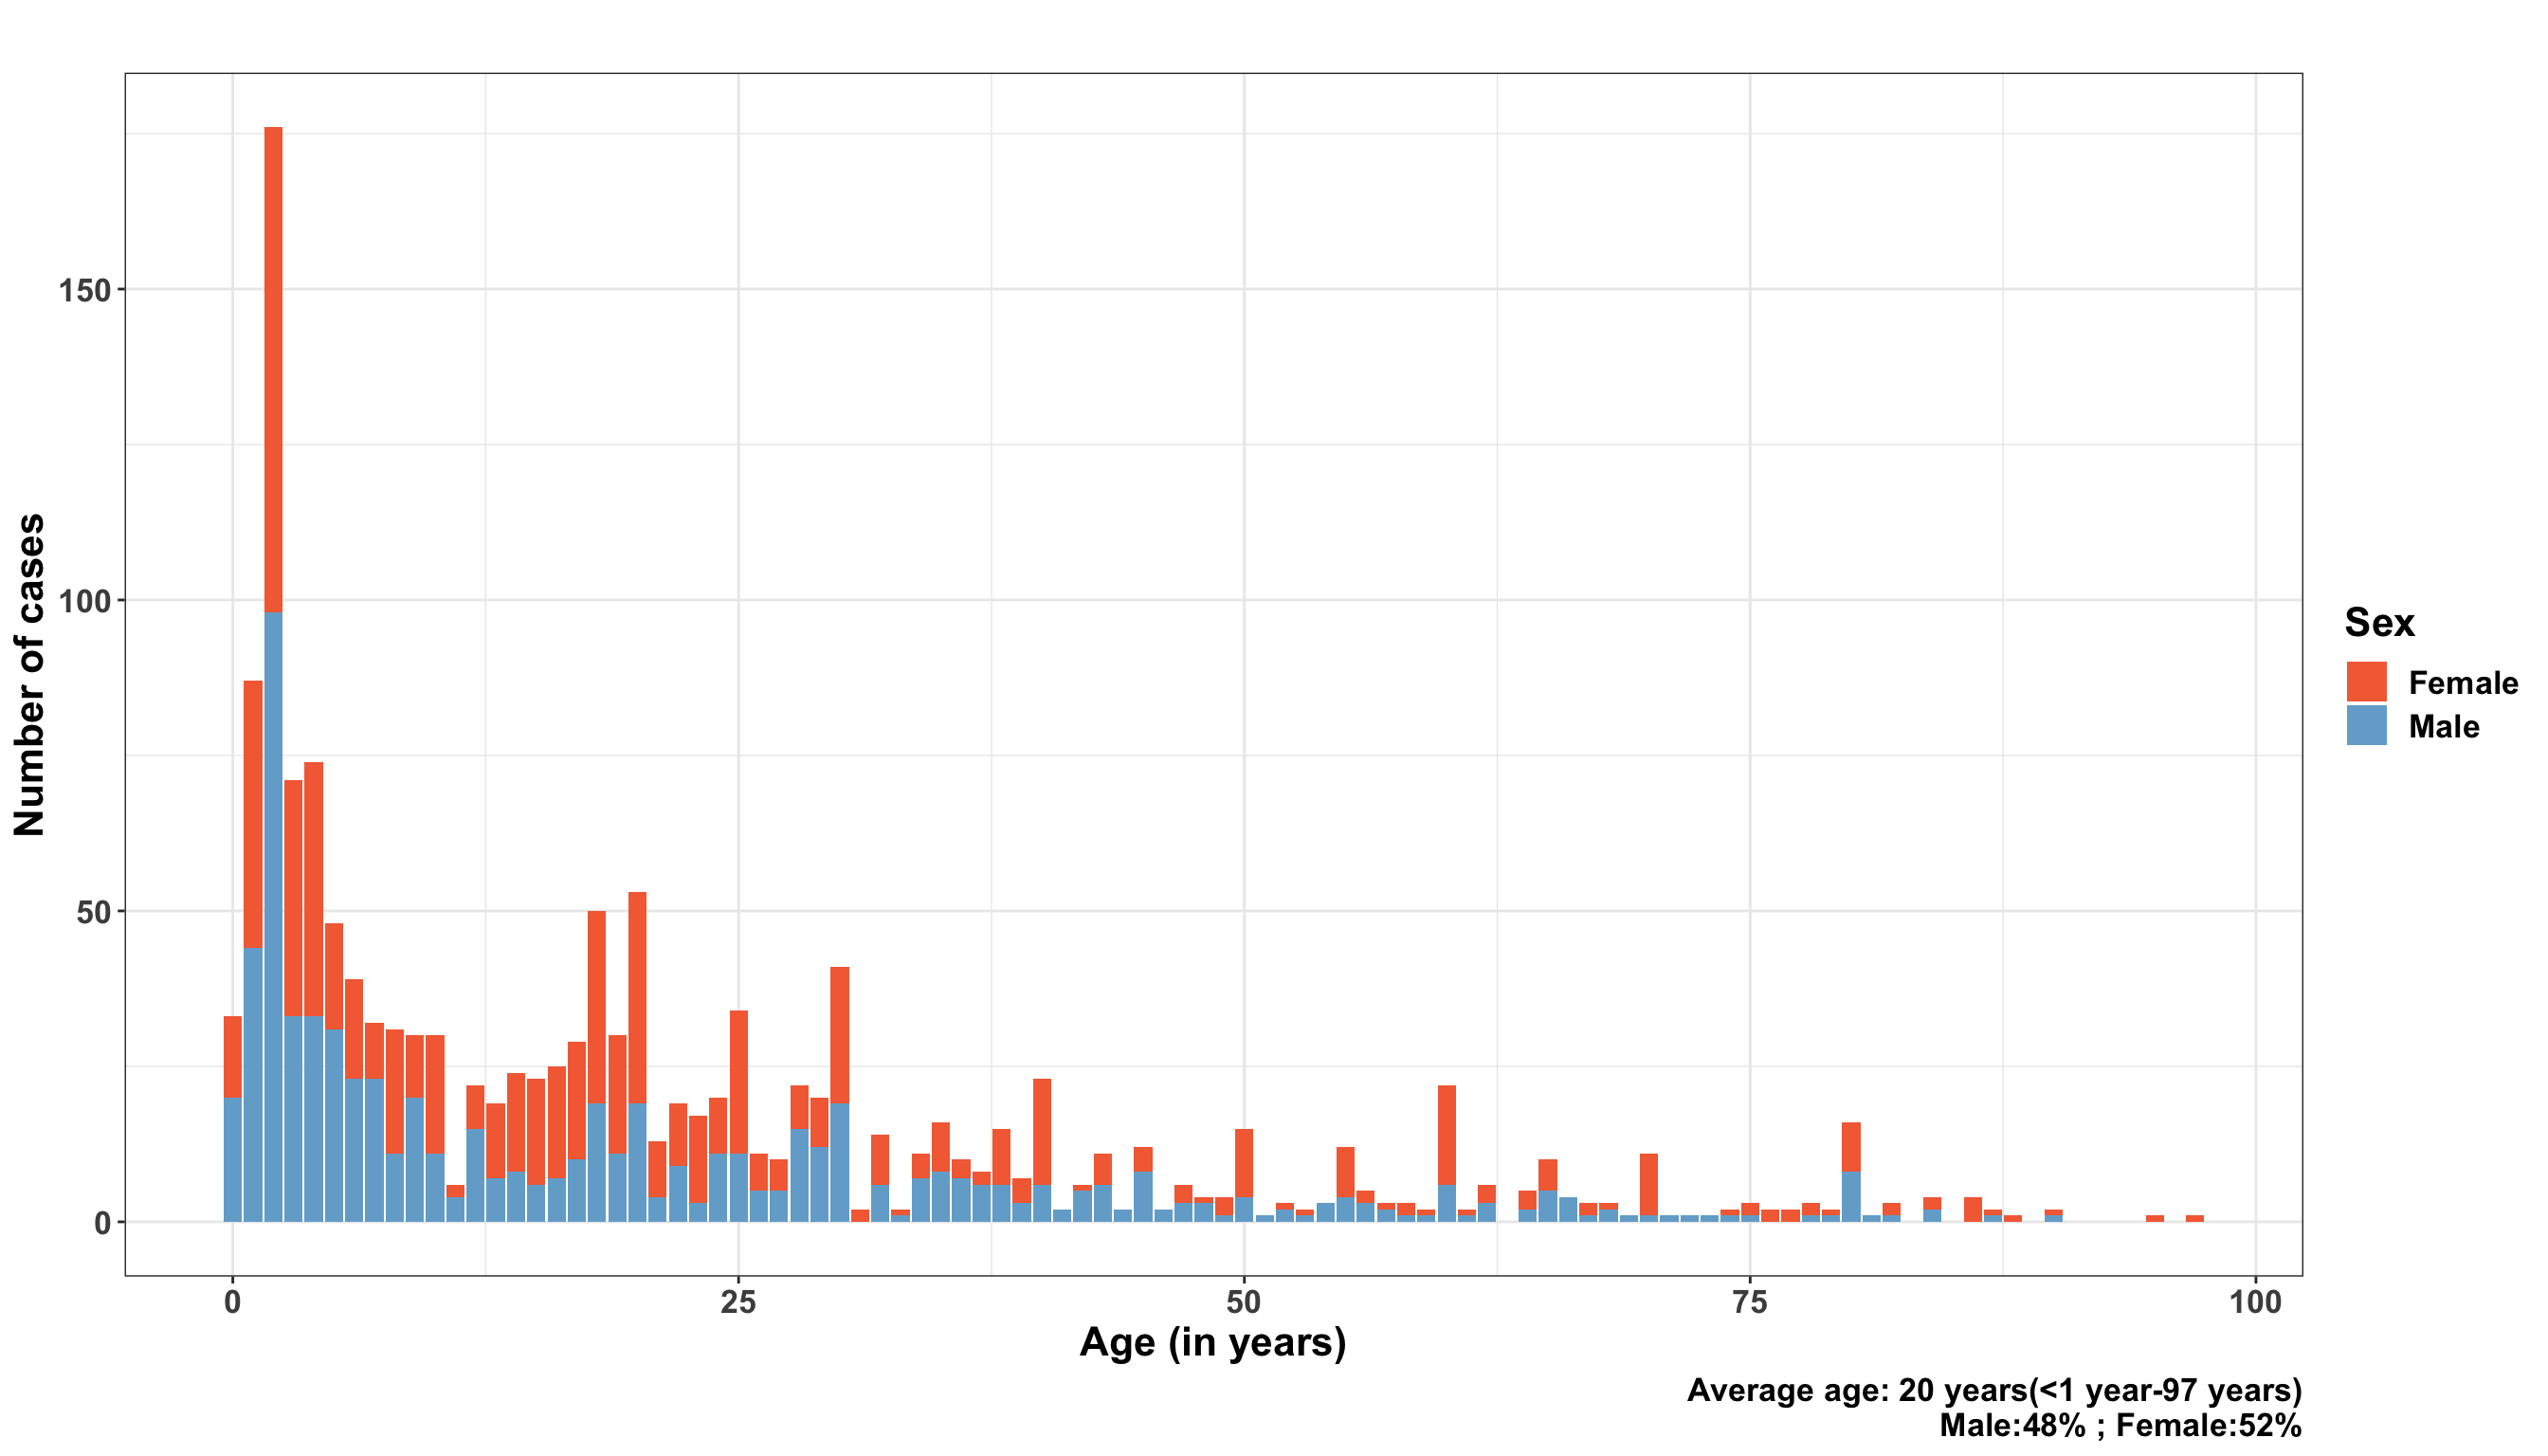
\includegraphics{_main_files/figure-latex/unnamed-chunk-54-1.pdf}

\hypertarget{spatial-distribution-8}{%
\section{Spatial distribution}\label{spatial-distribution-8}}

The spatial distribution of these cases at subcounty level is as shown:

\hypertarget{meru}{%
\chapter{Meru}\label{meru}}

\hypertarget{cases-over-time-9}{%
\section{Cases over time}\label{cases-over-time-9}}

As at 2023-03-23, there were 85 cases reported in Meru County.

This is shown in the graph below:

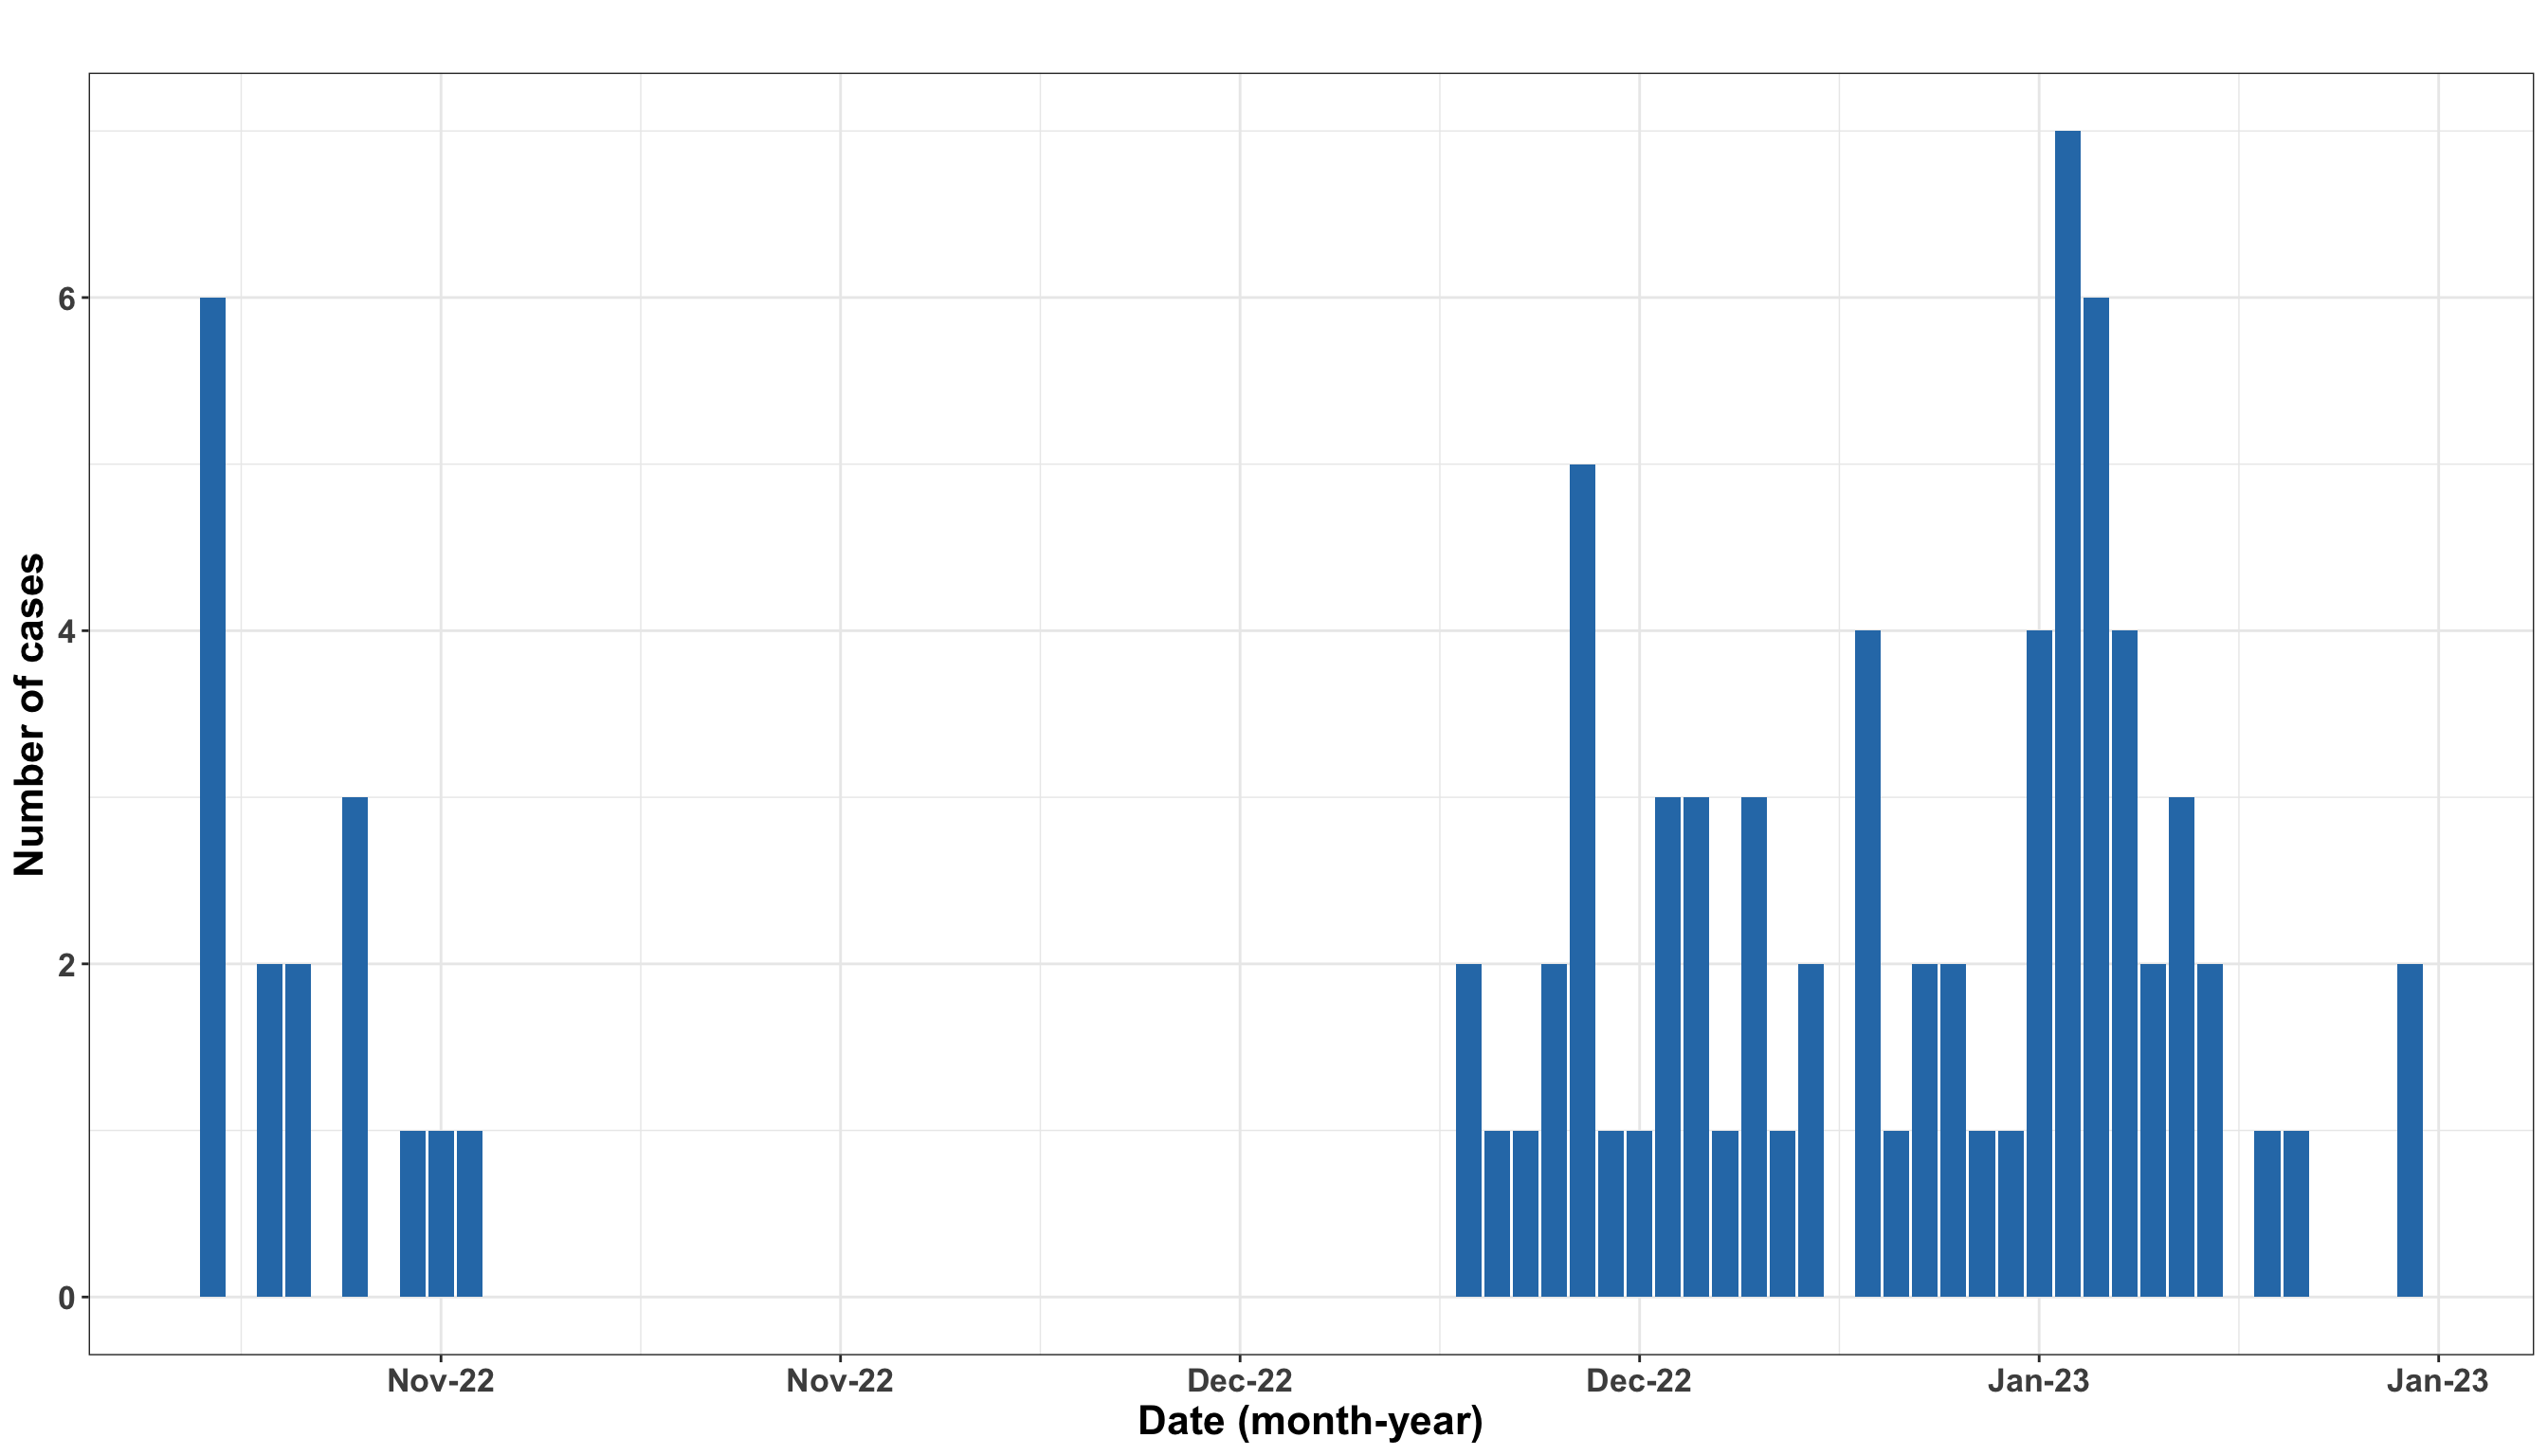
\includegraphics{_main_files/figure-latex/unnamed-chunk-58-1.pdf}

\hypertarget{demographic-distribution-9}{%
\section{Demographic distribution}\label{demographic-distribution-9}}

The stratification of these cases by age and sex is as shown:

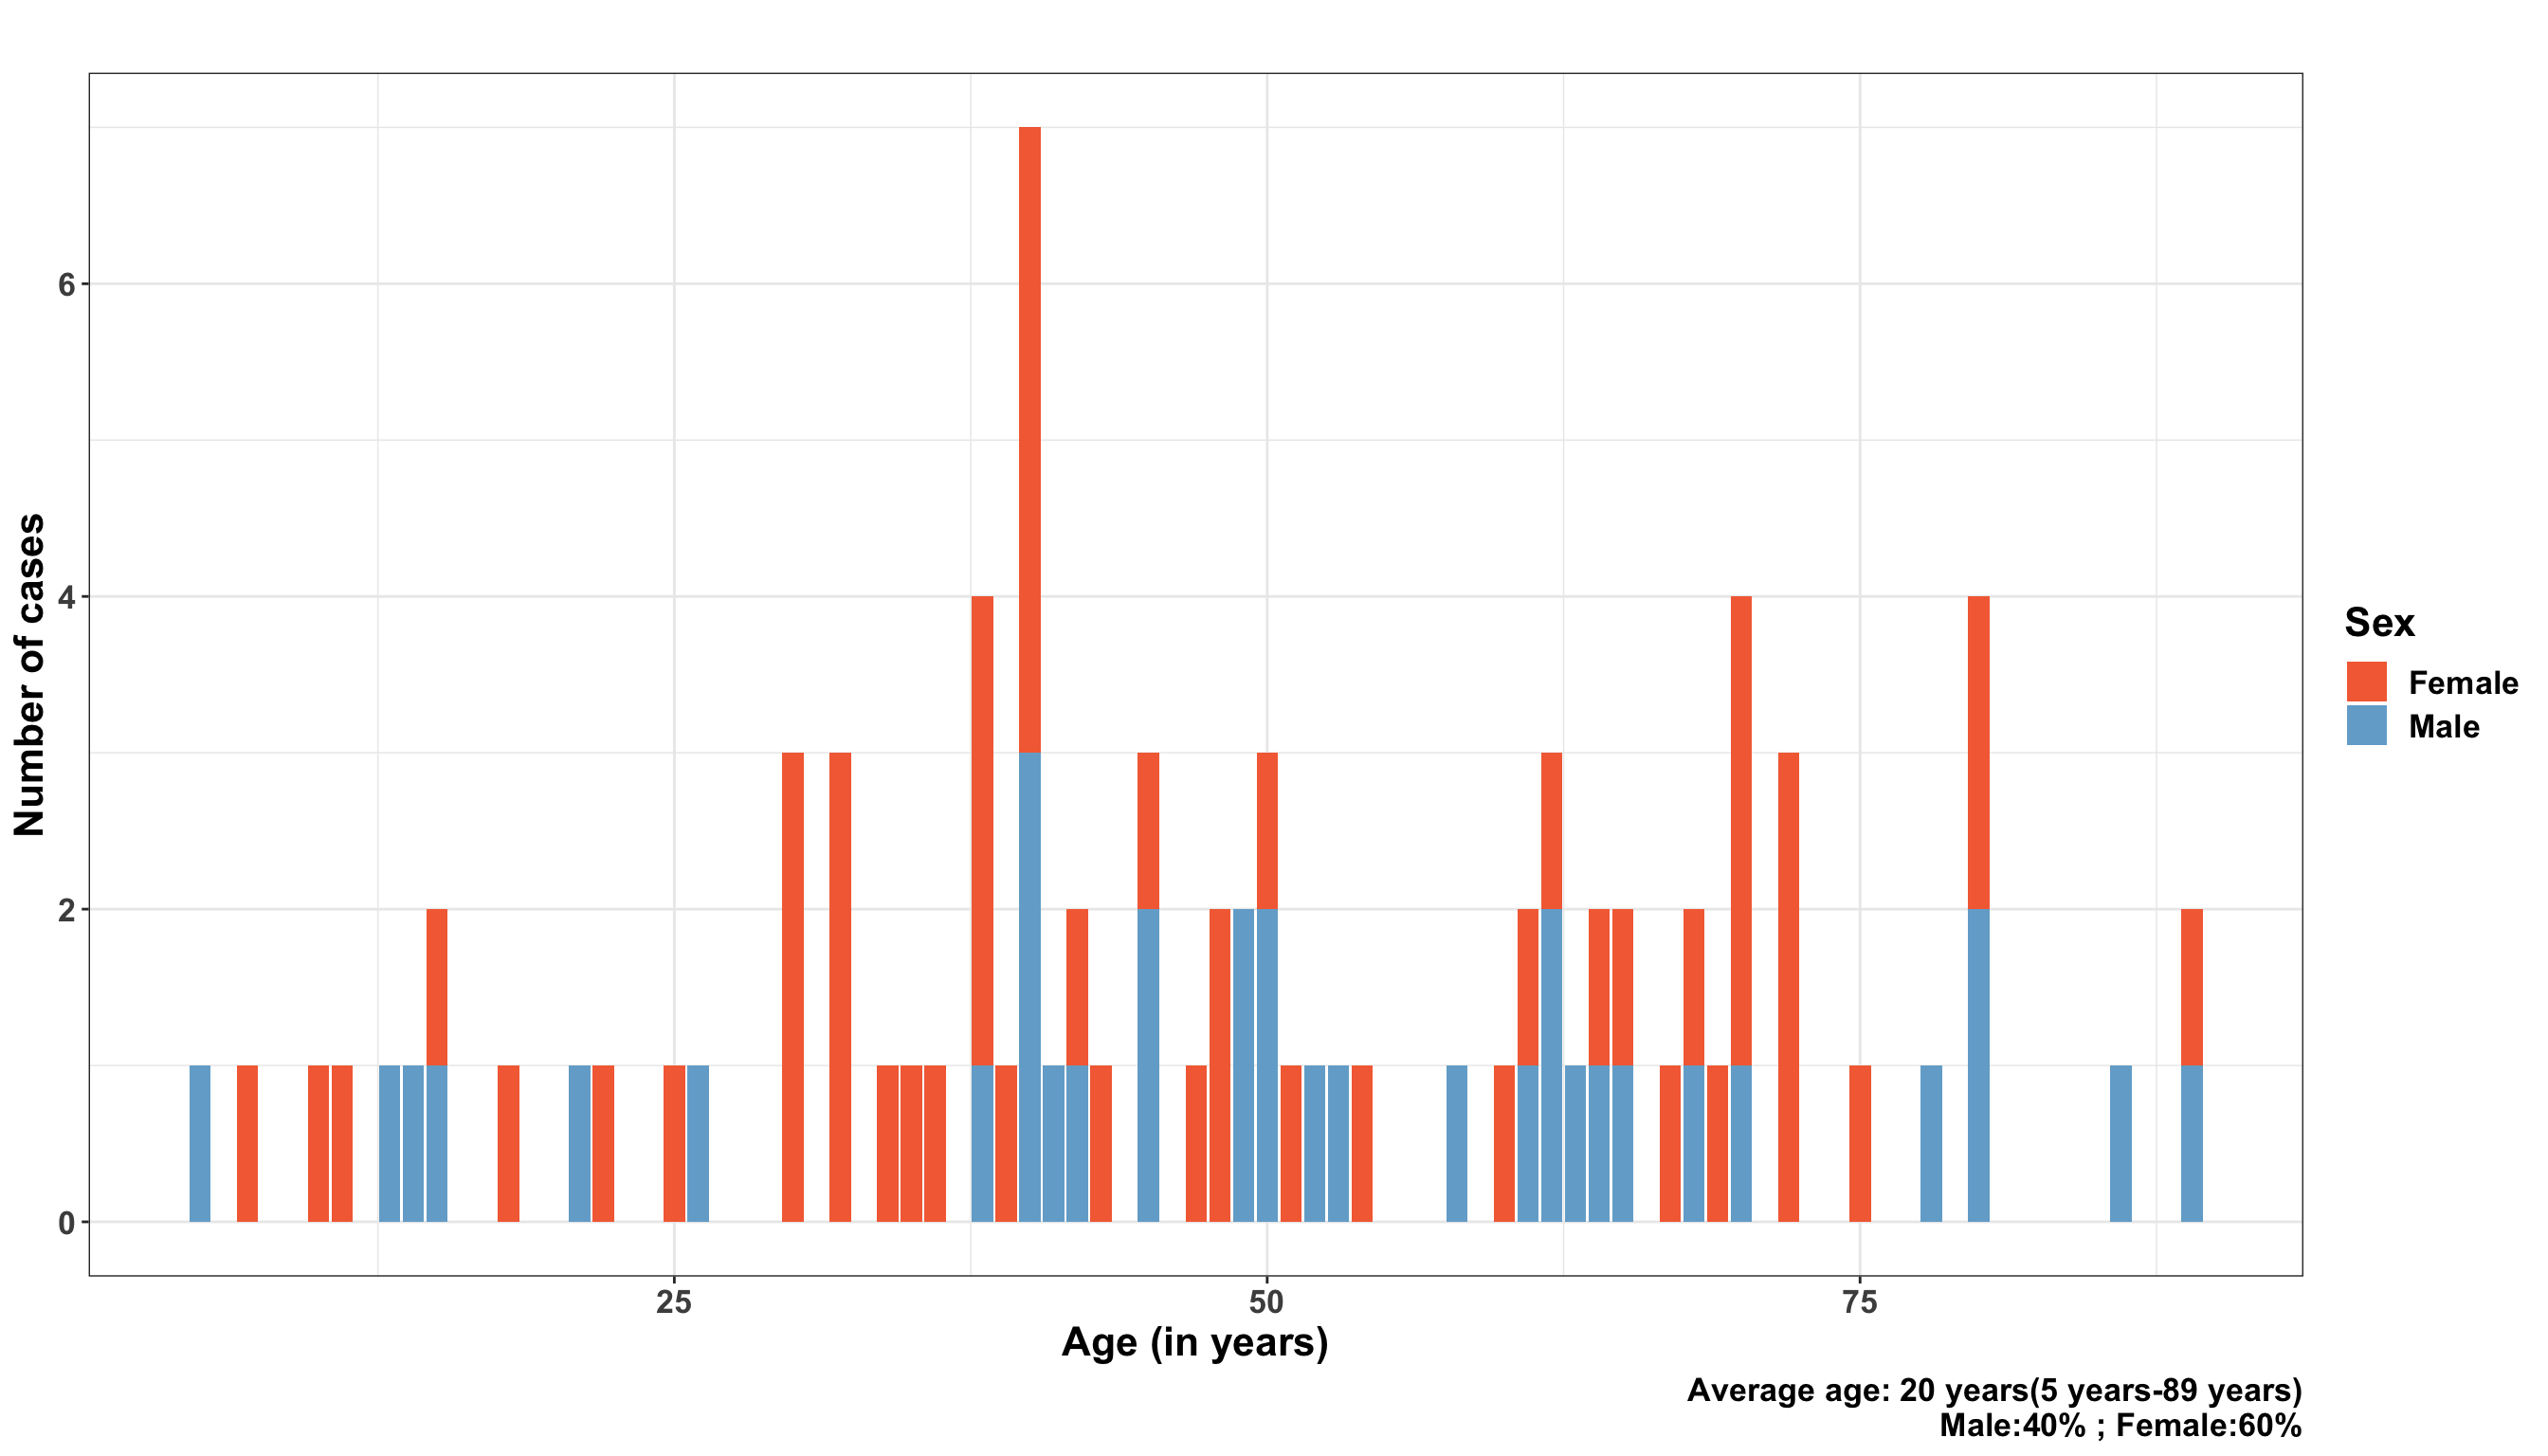
\includegraphics{_main_files/figure-latex/unnamed-chunk-60-1.pdf}

\hypertarget{spatial-distribution-9}{%
\section{Spatial distribution}\label{spatial-distribution-9}}

The spatial distribution of these cases at subcounty level is as shown:

\hypertarget{muranga}{%
\chapter{Murang'a}\label{muranga}}

\hypertarget{cases-over-time-10}{%
\section{Cases over time}\label{cases-over-time-10}}

As at 2023-03-23, there were 43 cases reported in Murang'a County.

This is shown in the graph below:

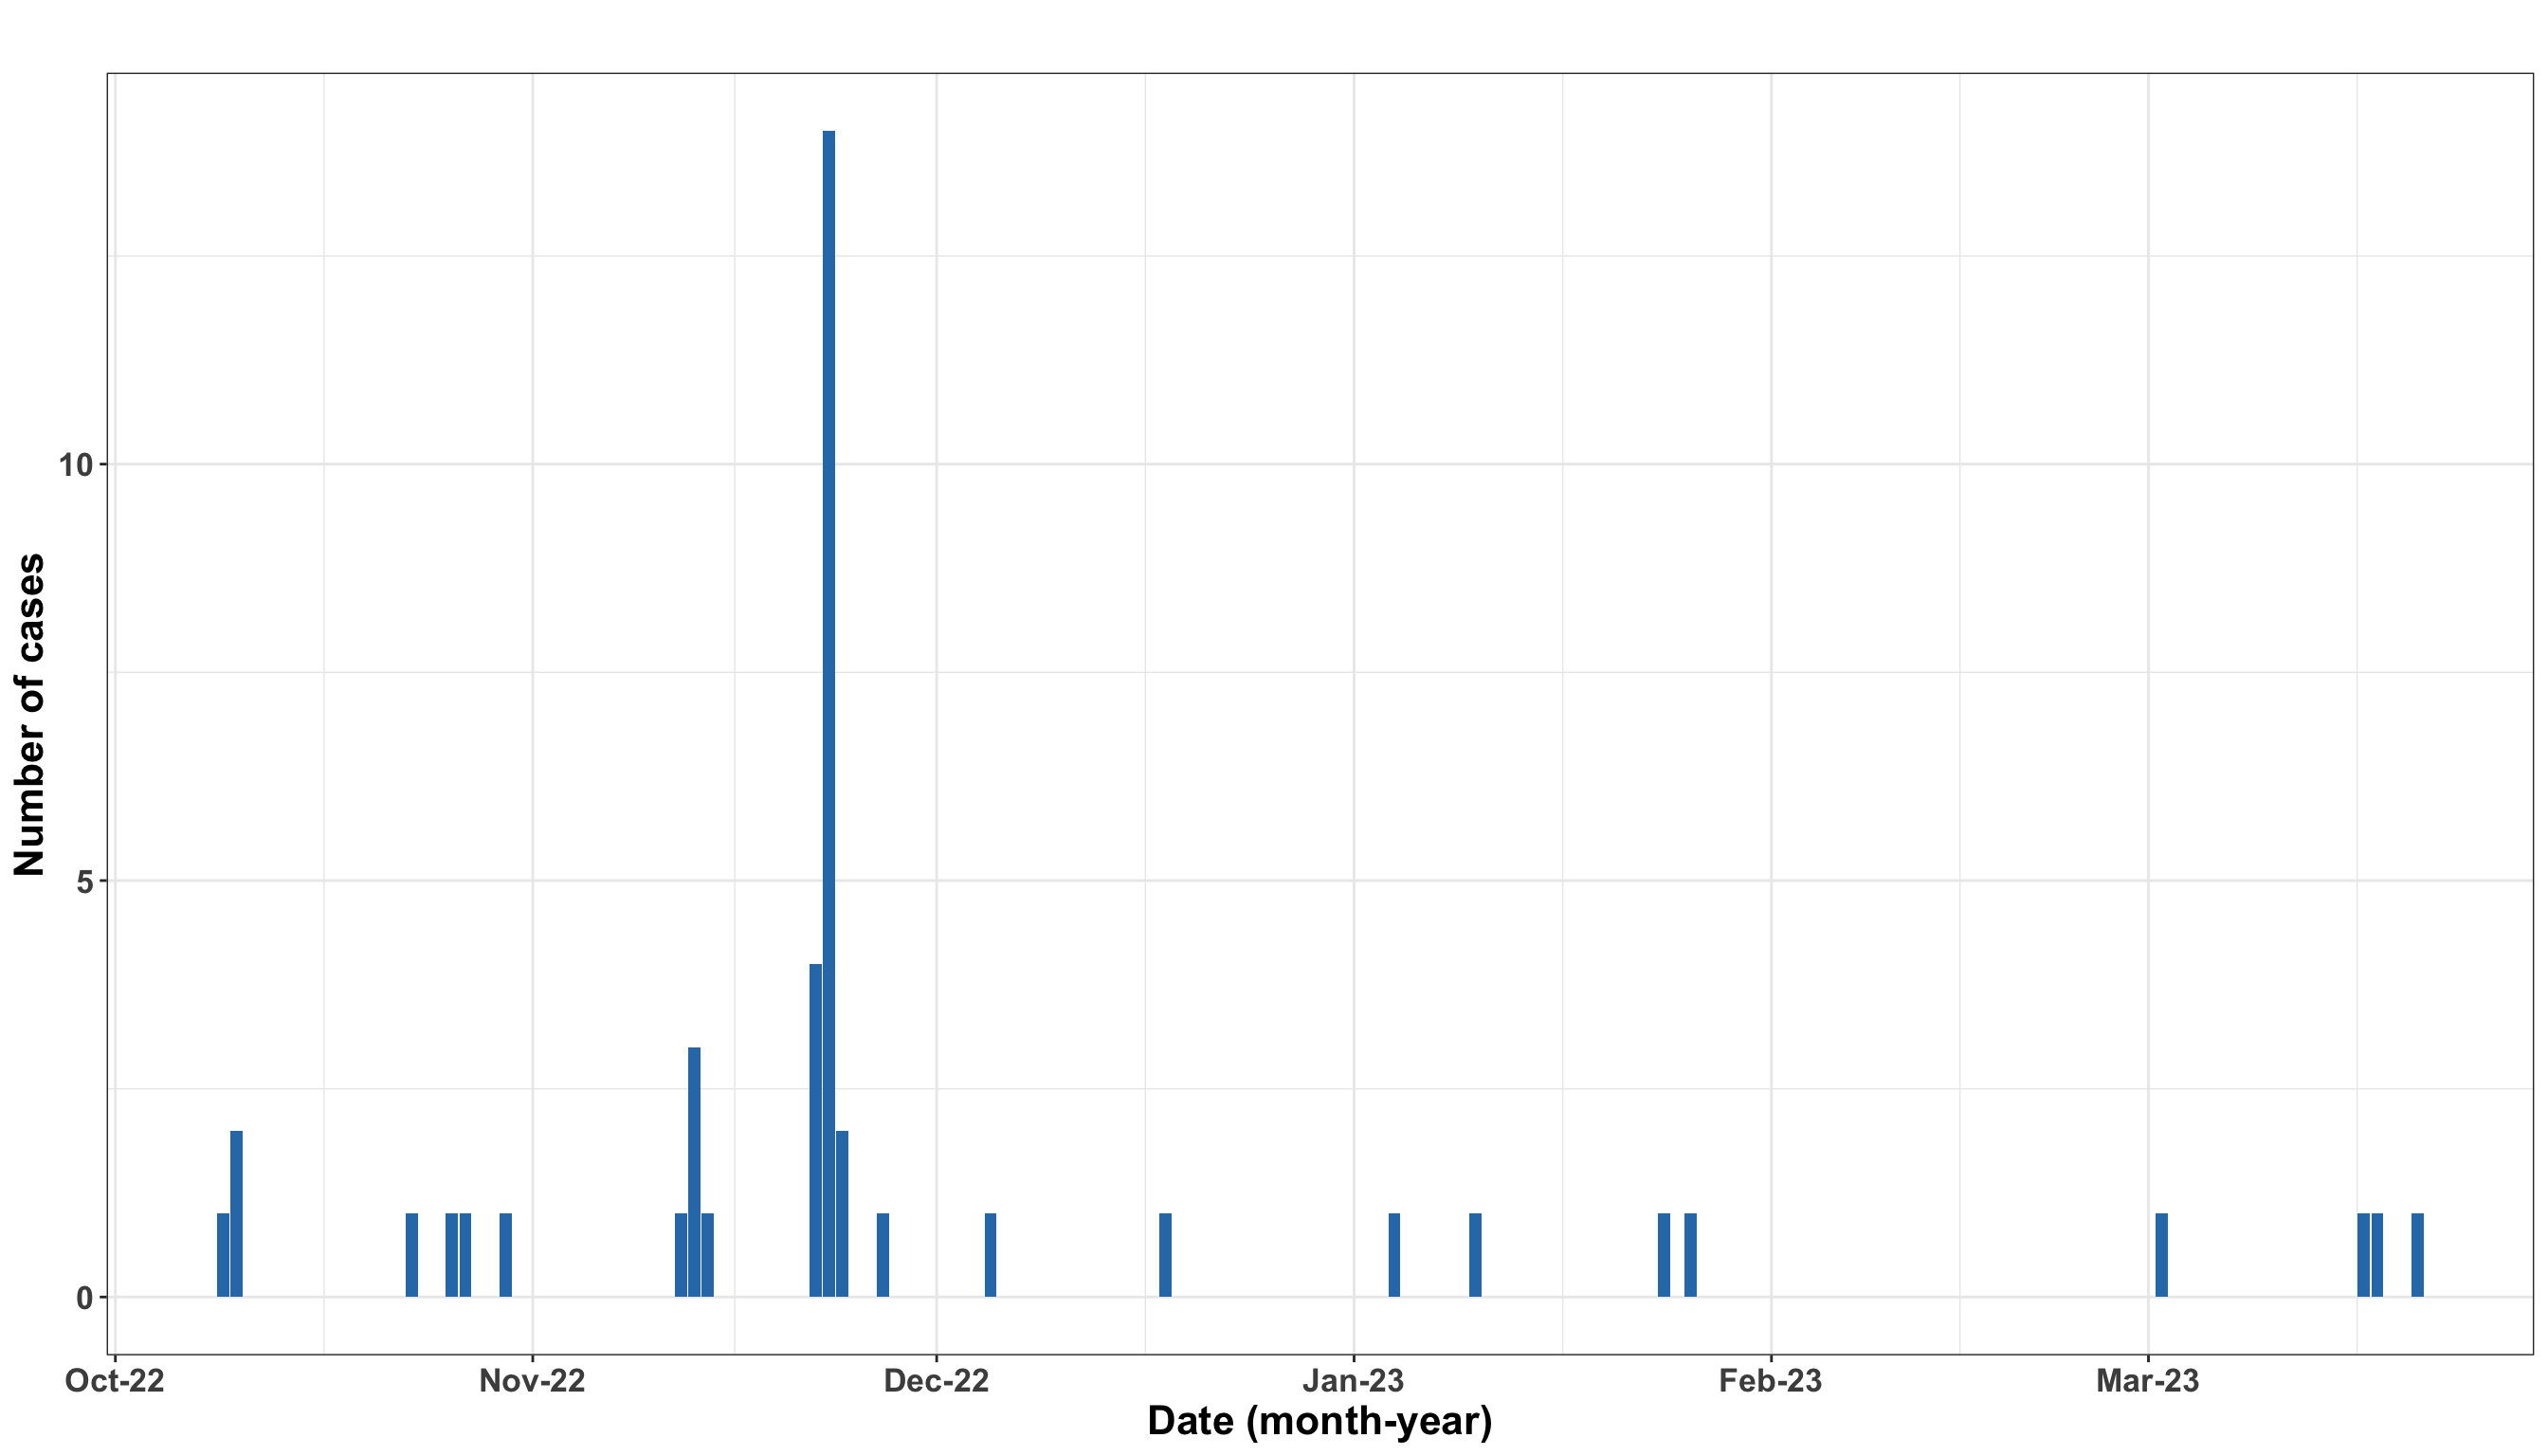
\includegraphics{_main_files/figure-latex/unnamed-chunk-64-1.pdf}

\hypertarget{demographic-distribution-10}{%
\section{Demographic distribution}\label{demographic-distribution-10}}

The stratification of these cases by age and sex is as shown:

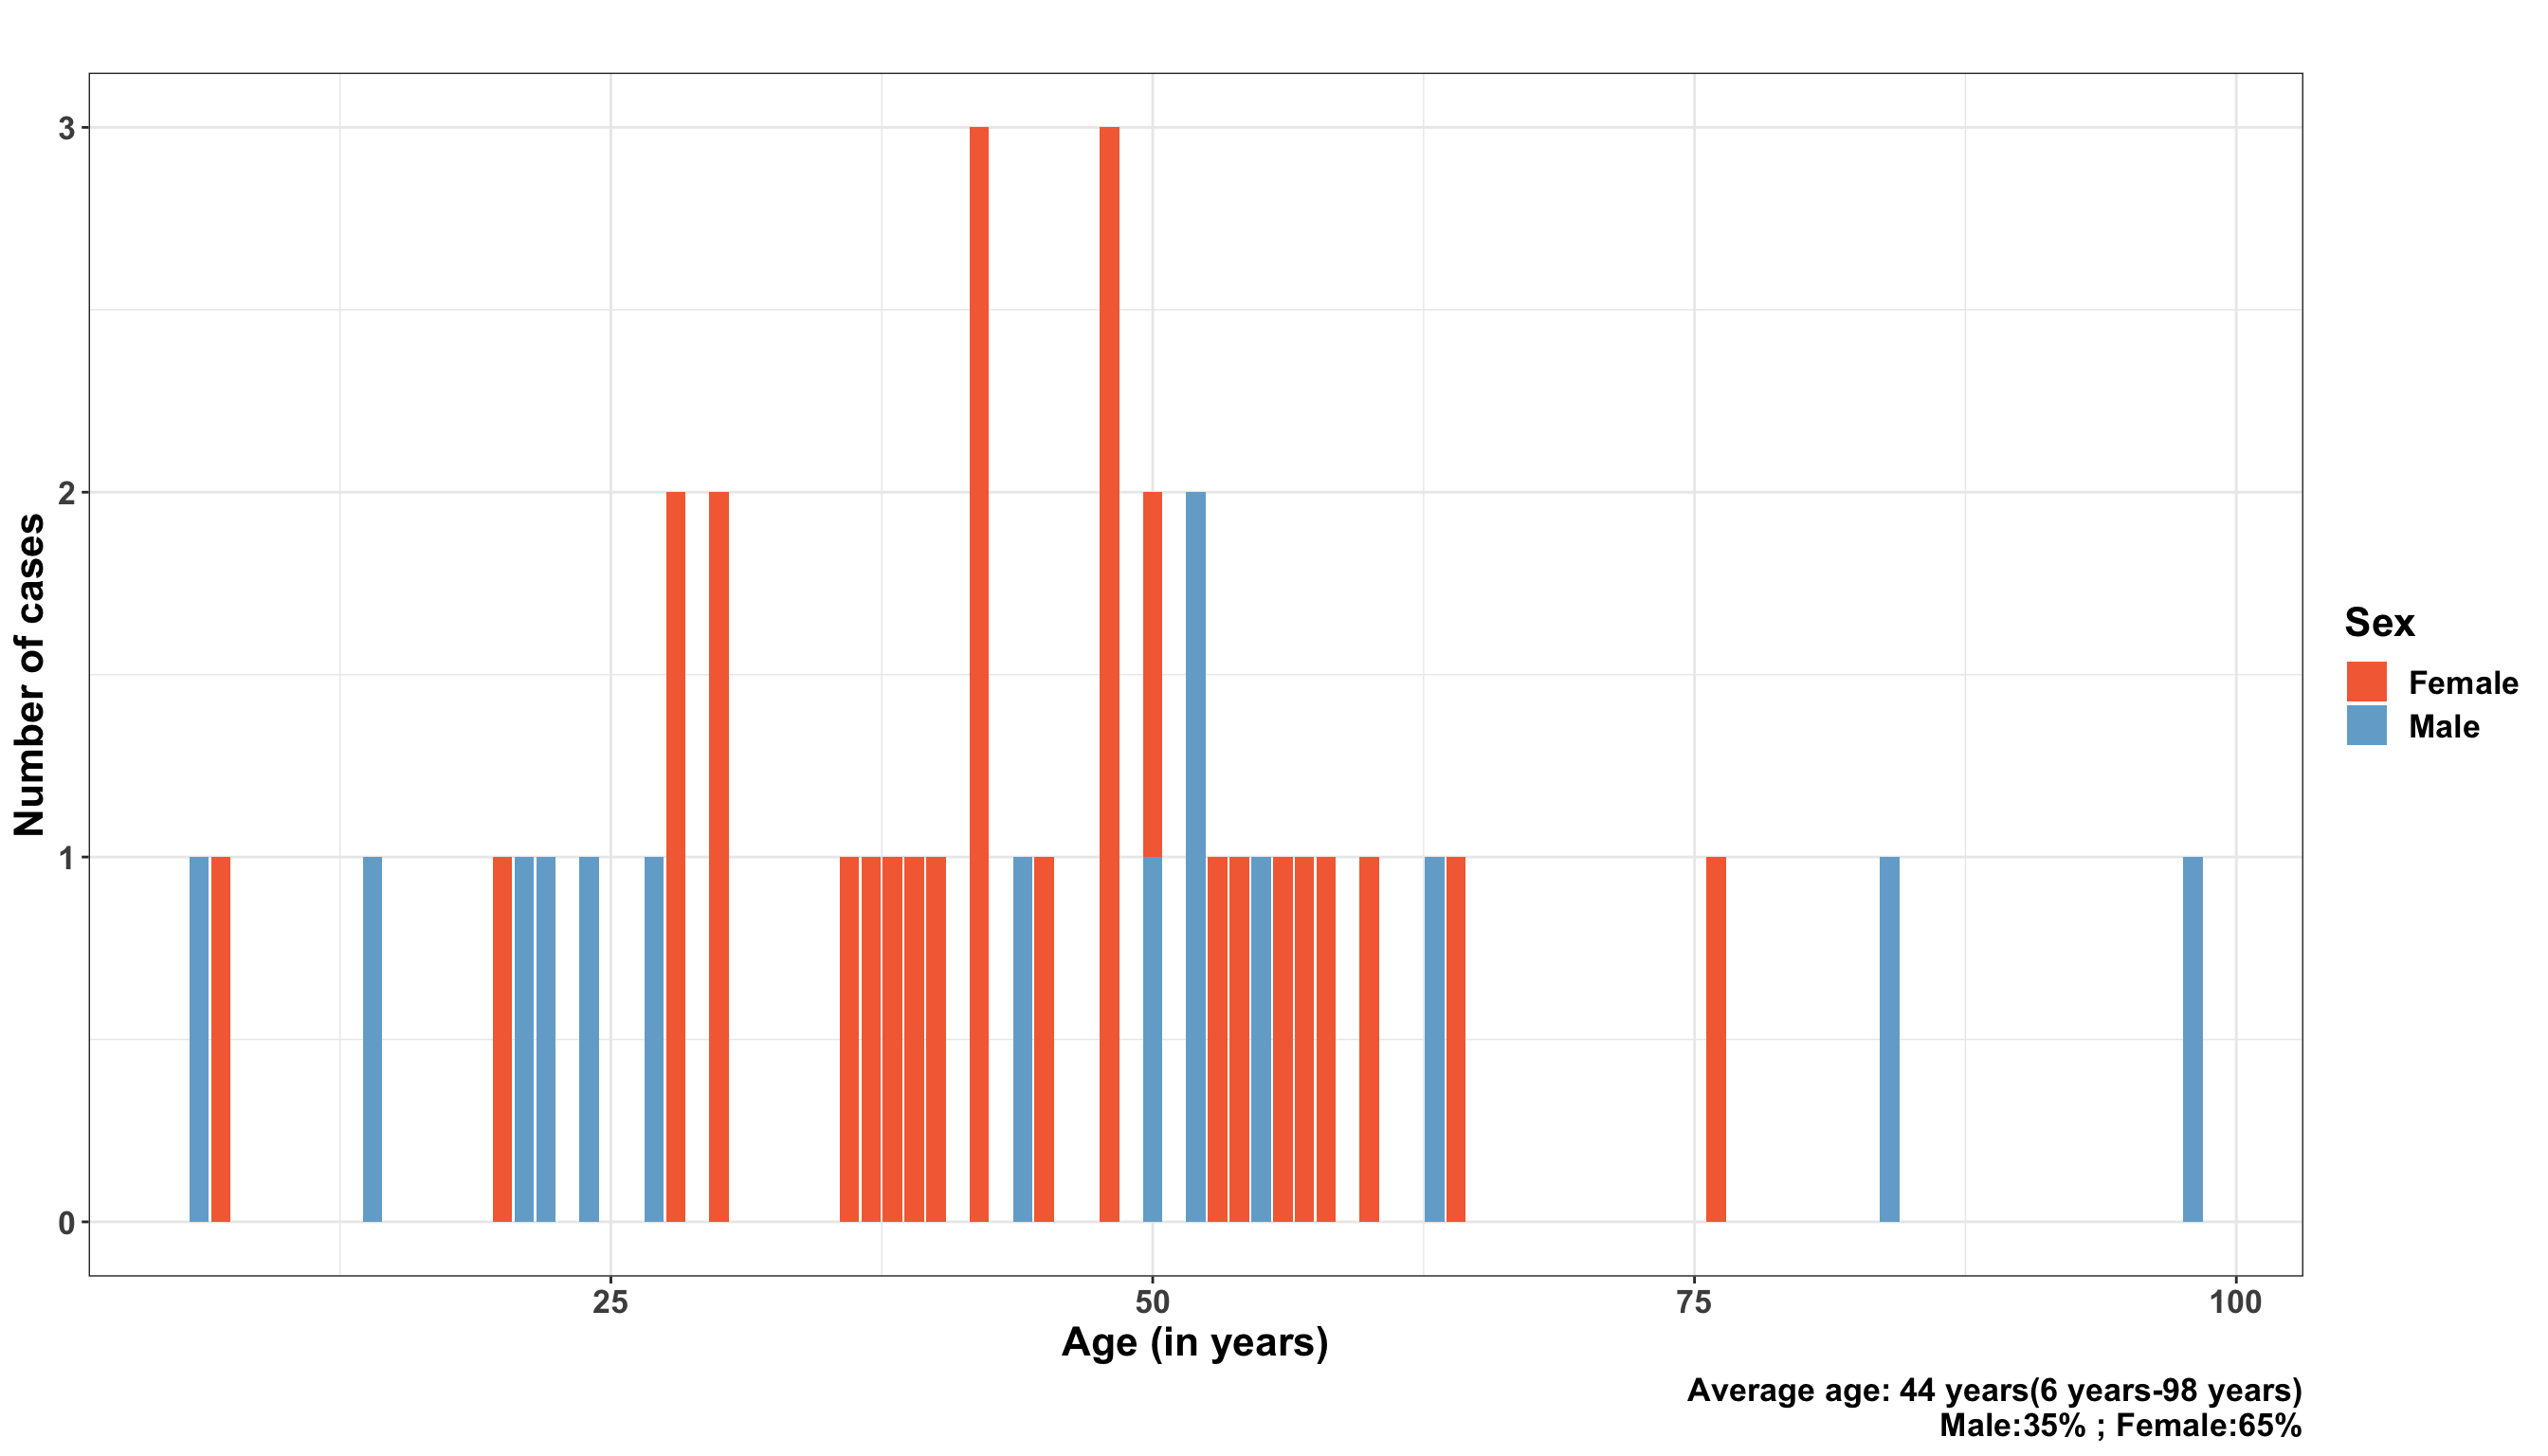
\includegraphics{_main_files/figure-latex/unnamed-chunk-66-1.pdf}

\hypertarget{spatial-distribution-10}{%
\section{Spatial distribution}\label{spatial-distribution-10}}

The spatial distribution of these cases at subcounty level is as shown:

\hypertarget{nairobi}{%
\chapter{Nairobi}\label{nairobi}}

\hypertarget{cases-over-time-11}{%
\section{Cases over time}\label{cases-over-time-11}}

As at 2023-03-23, there were 1186 cases reported in Nairobi County.

This is shown in the graph below:

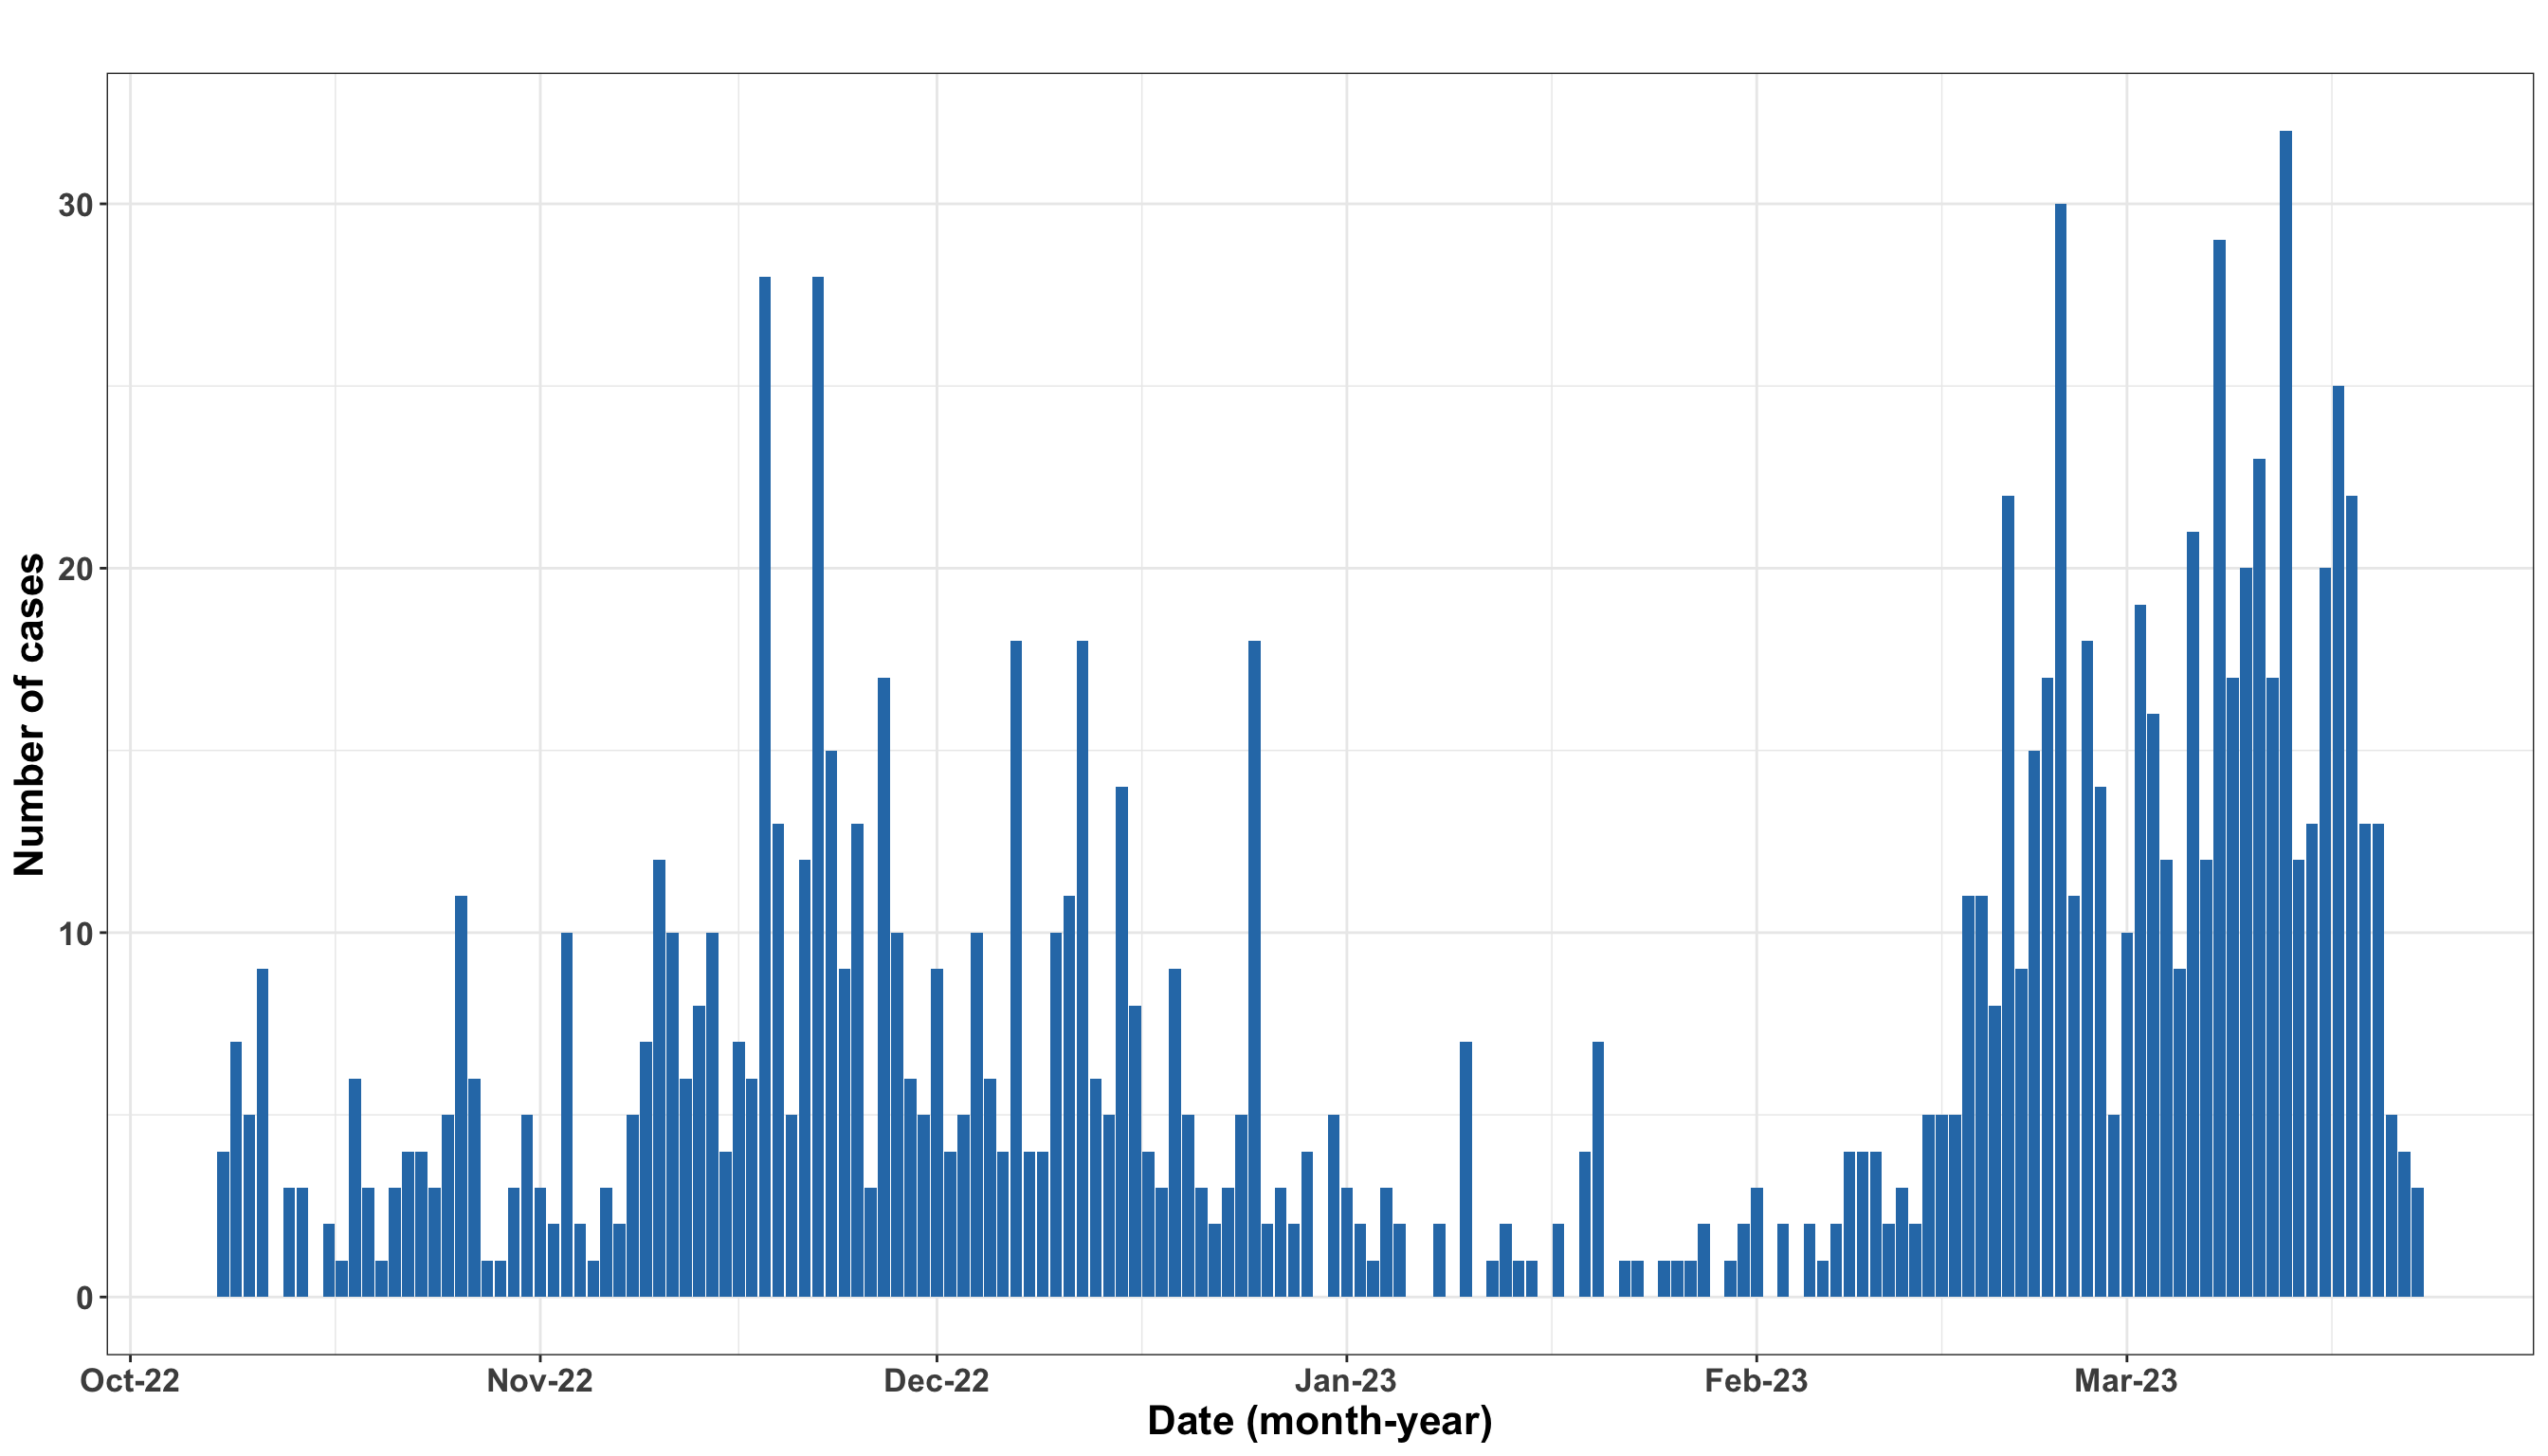
\includegraphics{_main_files/figure-latex/unnamed-chunk-70-1.pdf}

\hypertarget{demographic-distribution-11}{%
\section{Demographic distribution}\label{demographic-distribution-11}}

The stratification of these cases by age and sex is as shown:

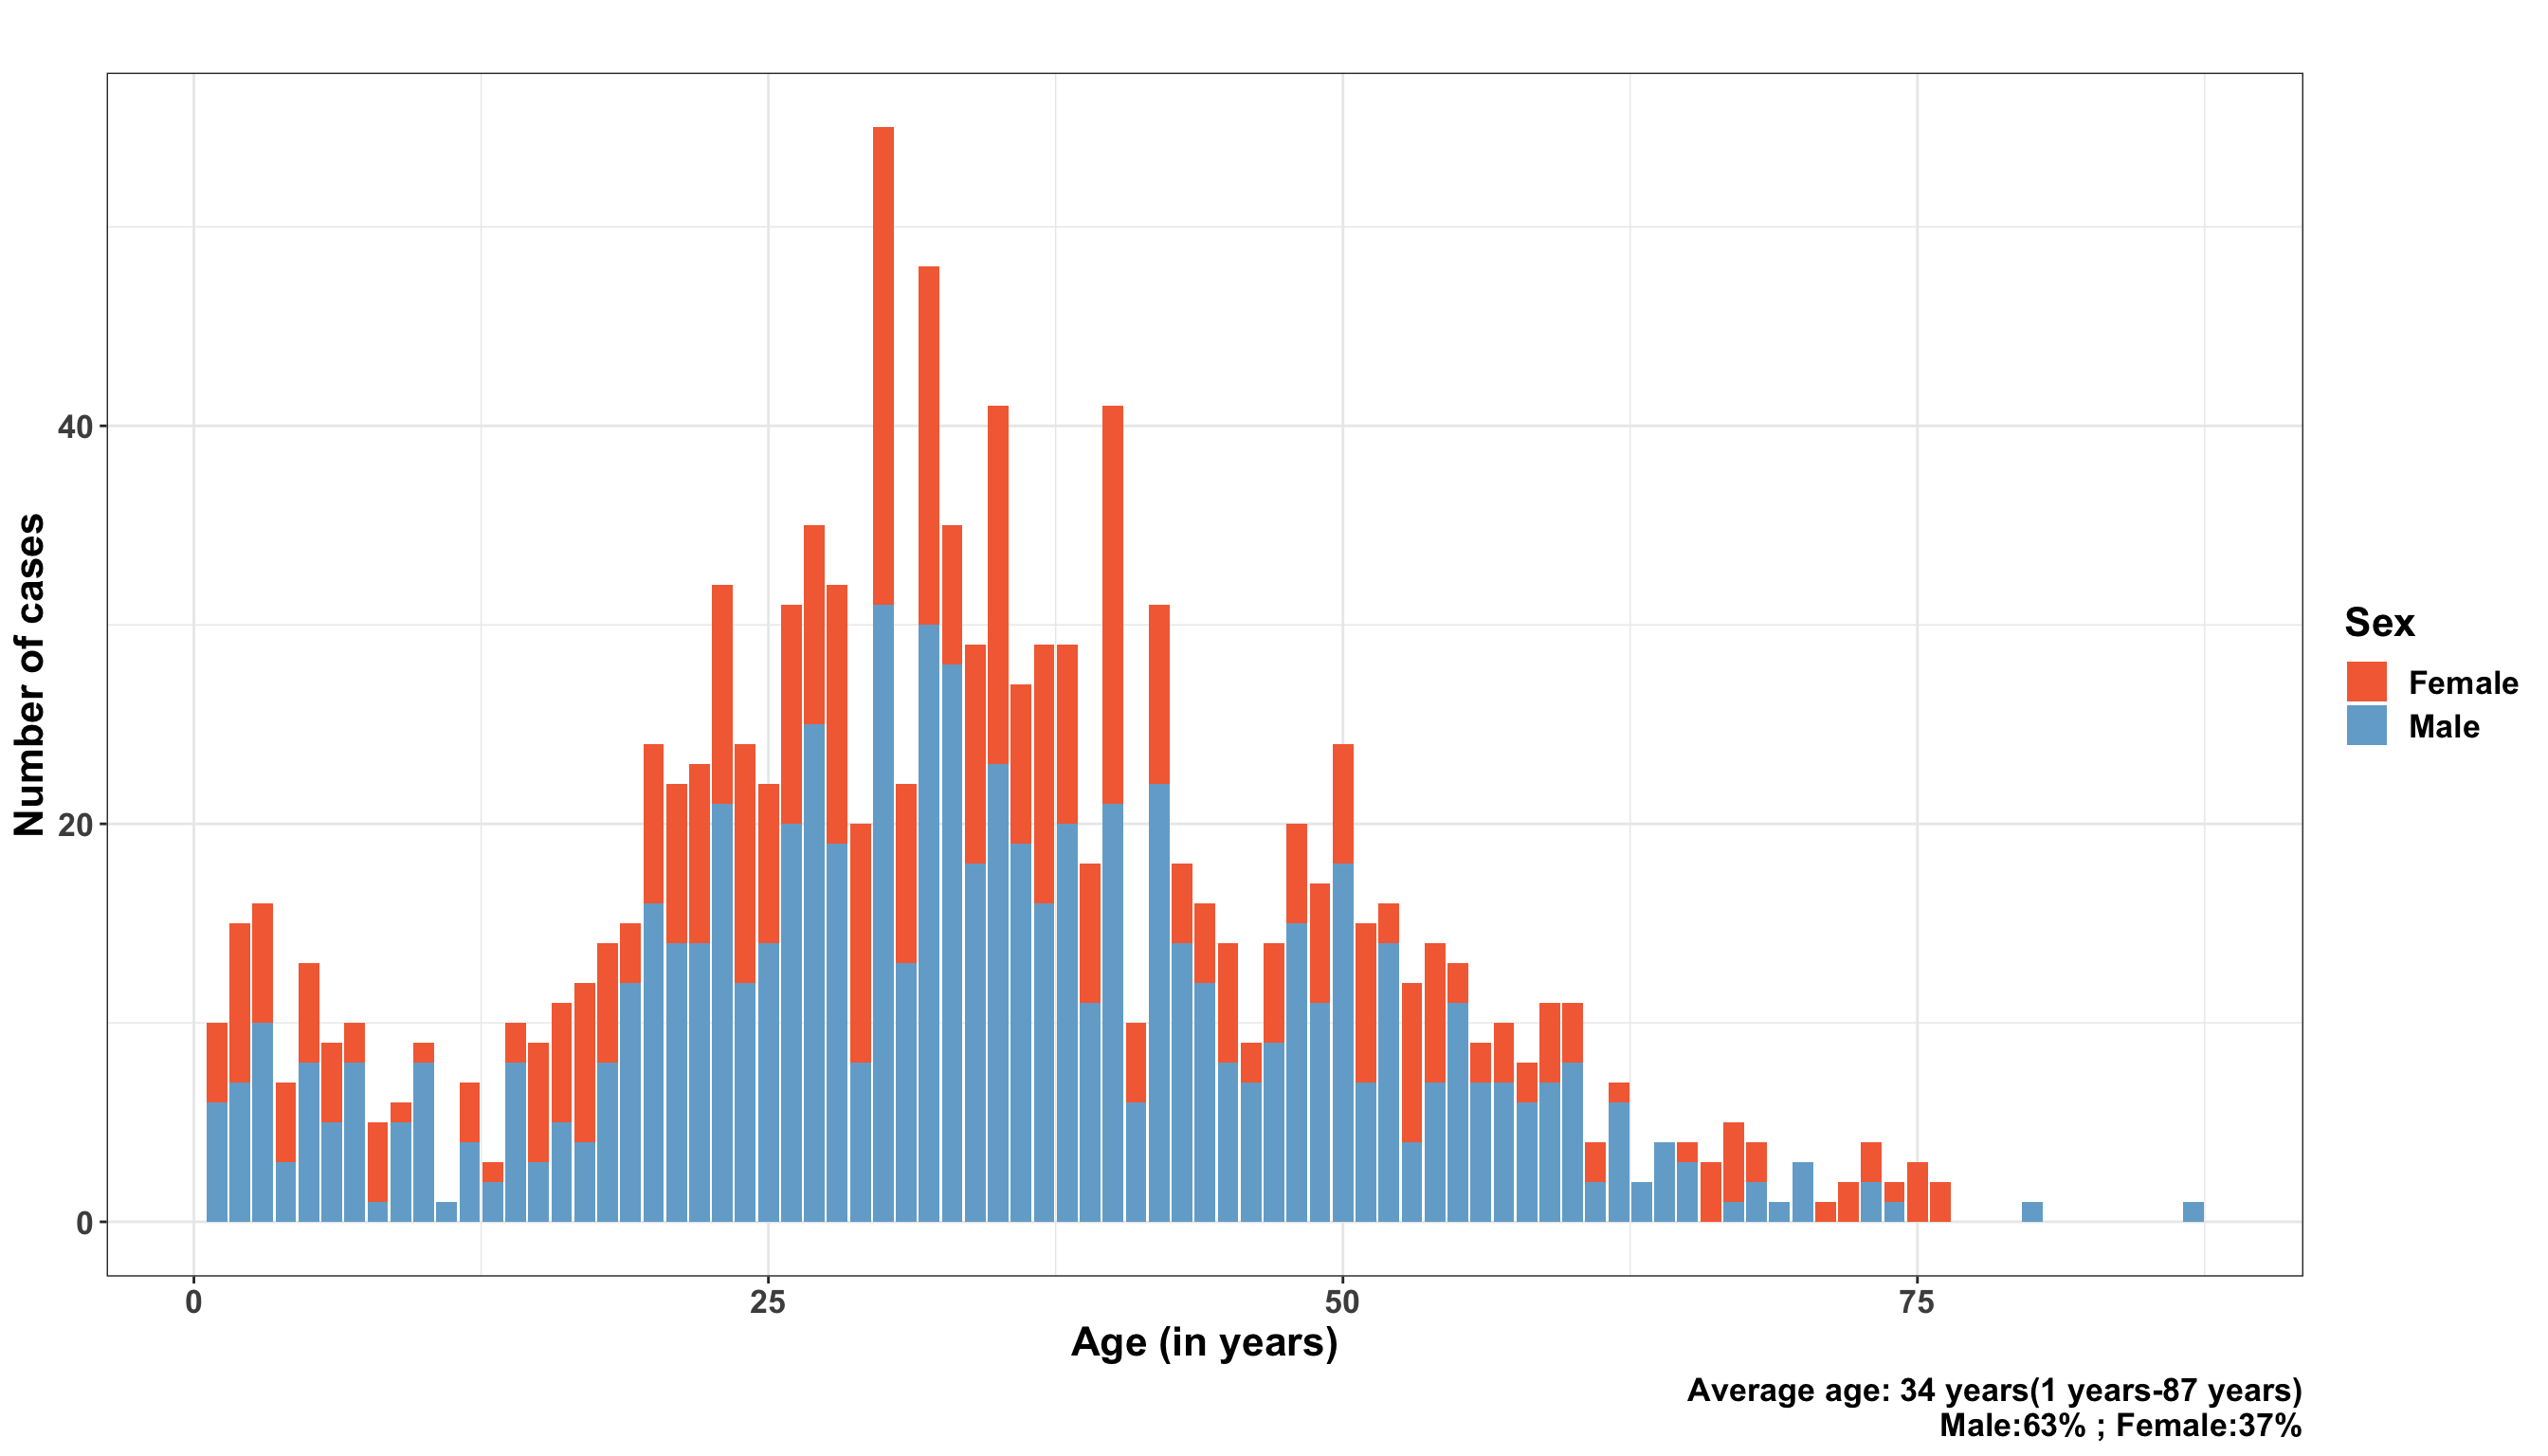
\includegraphics{_main_files/figure-latex/unnamed-chunk-72-1.pdf}

\hypertarget{spatial-distribution-11}{%
\section{Spatial distribution}\label{spatial-distribution-11}}

The spatial distribution of these cases at subcounty level is as shown:

\hypertarget{nakuru}{%
\chapter{Nakuru}\label{nakuru}}

\hypertarget{cases-over-time-12}{%
\section{Cases over time}\label{cases-over-time-12}}

As at 2023-03-23, there were 13 cases reported in Nakuru County.

This is shown in the graph below:

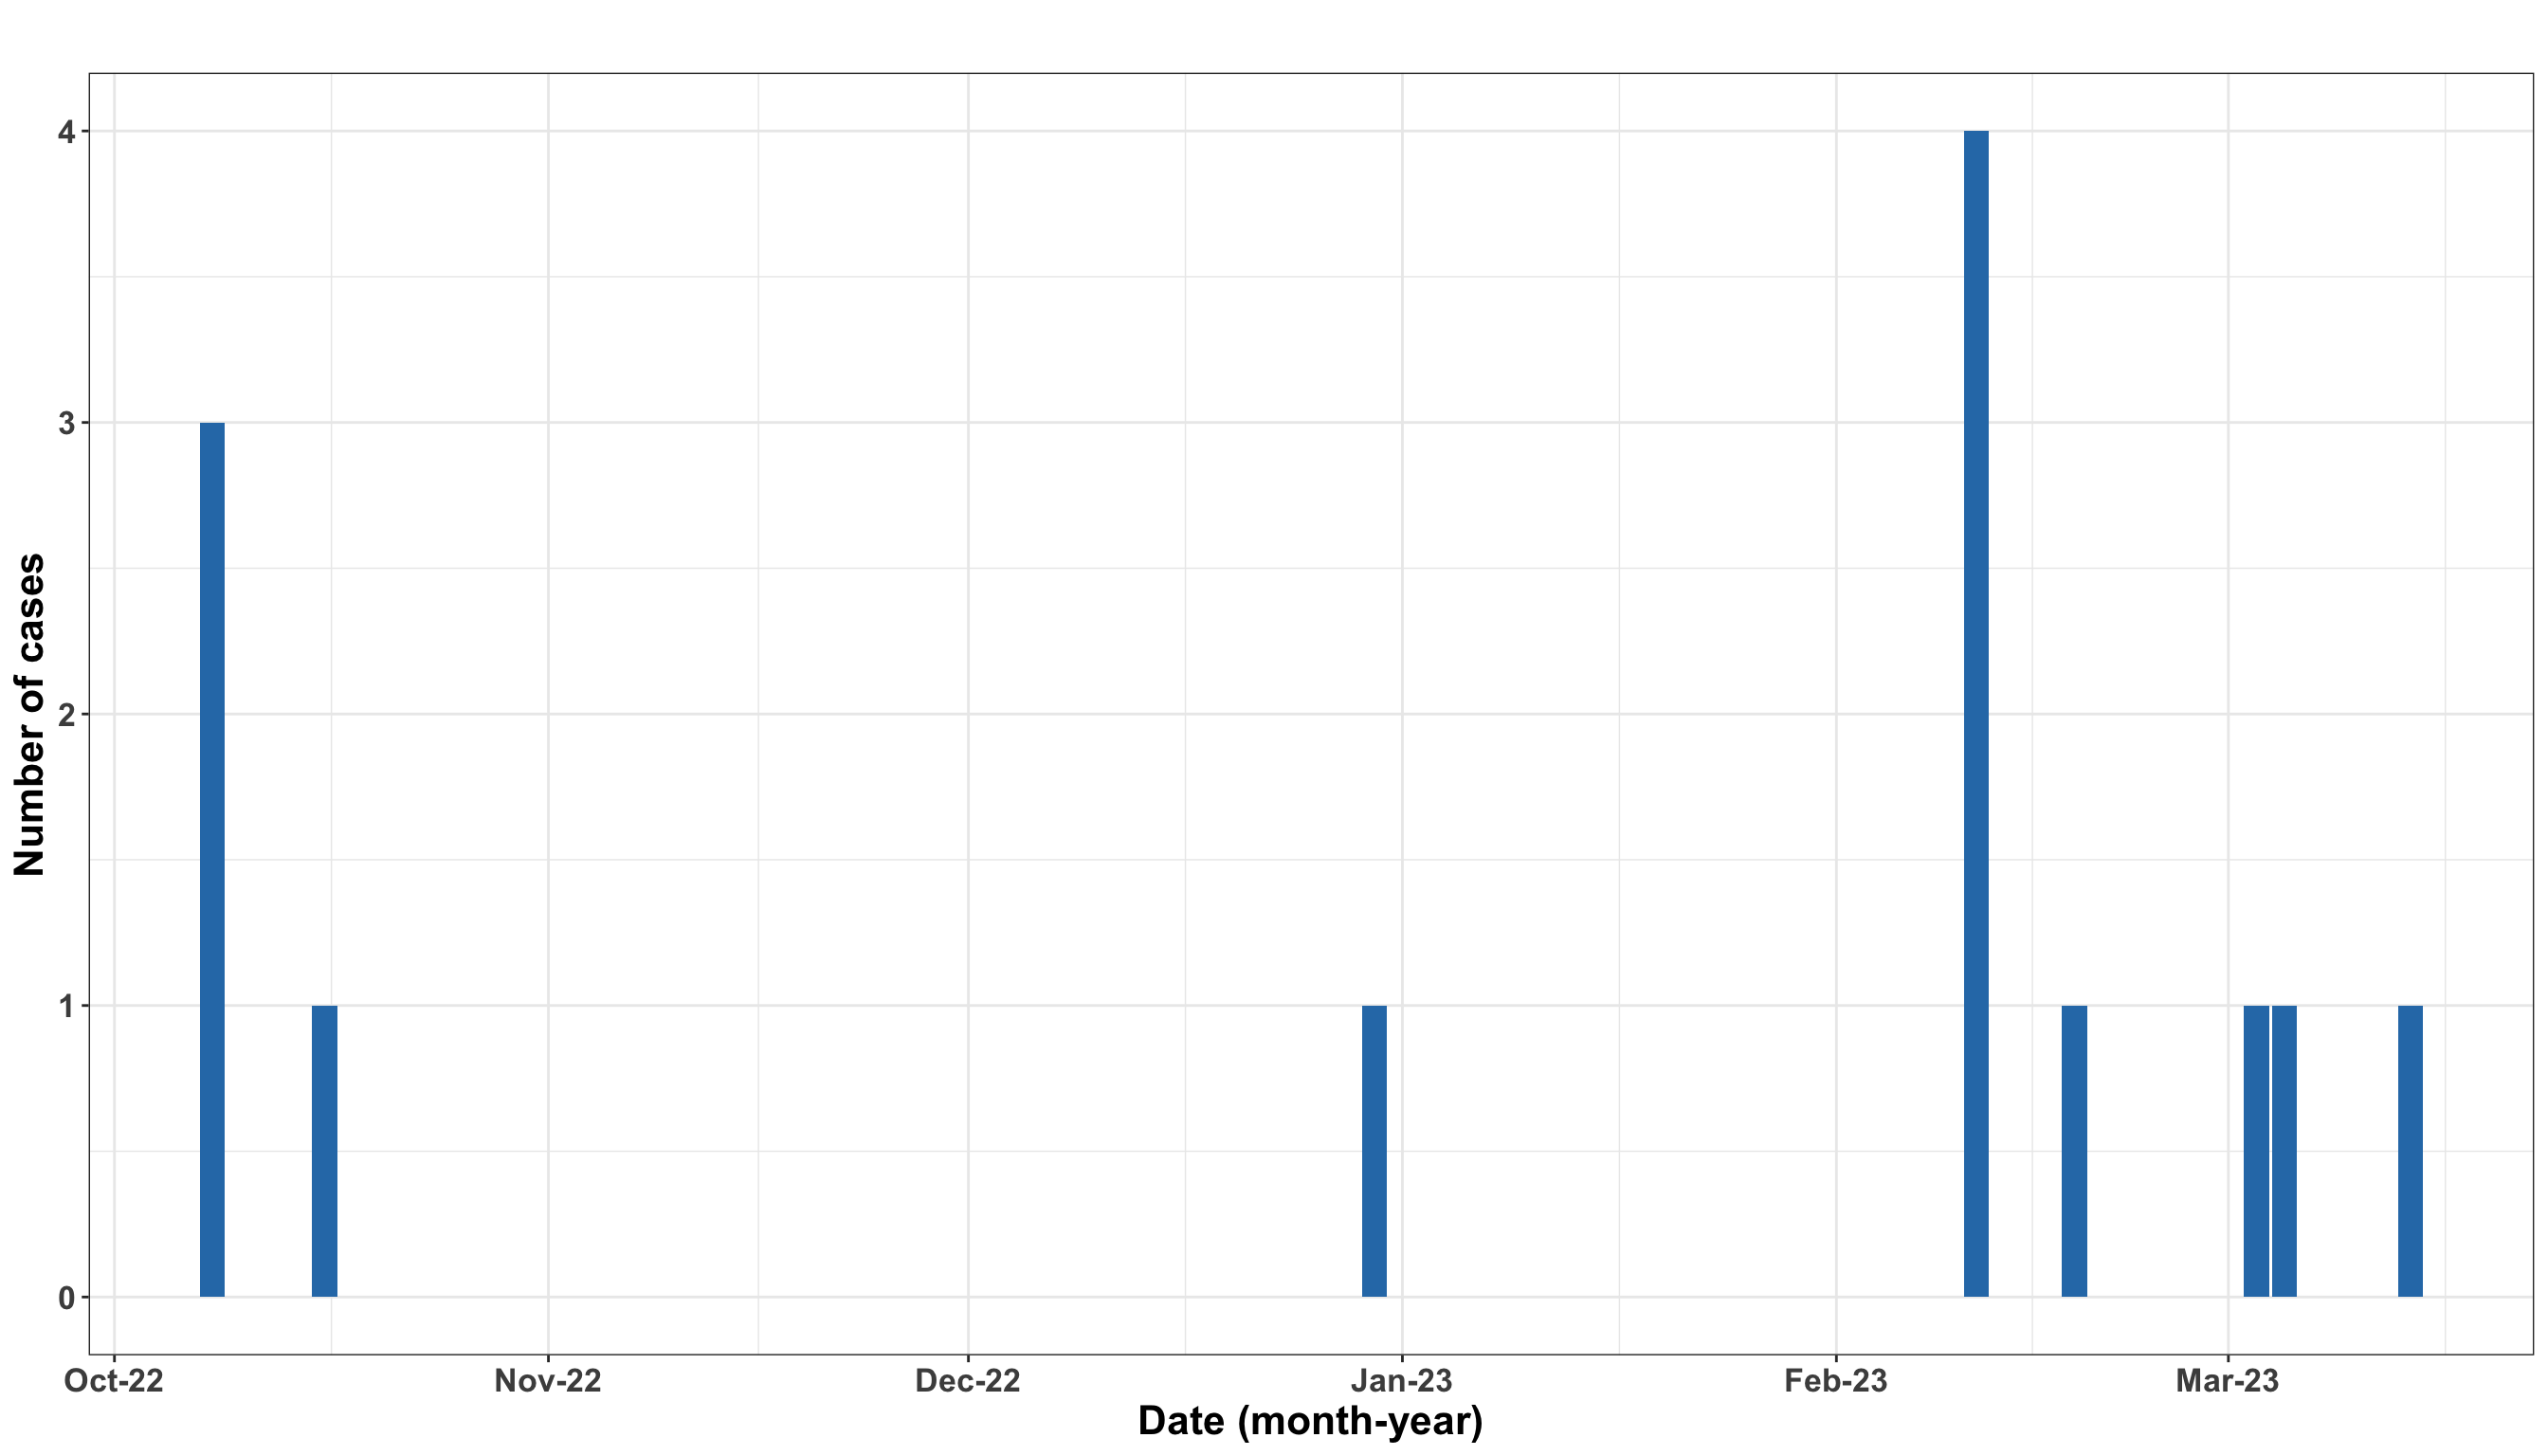
\includegraphics{_main_files/figure-latex/unnamed-chunk-76-1.pdf}

\hypertarget{demographic-distribution-12}{%
\section{Demographic distribution}\label{demographic-distribution-12}}

The stratification of these cases by age and sex is as shown:

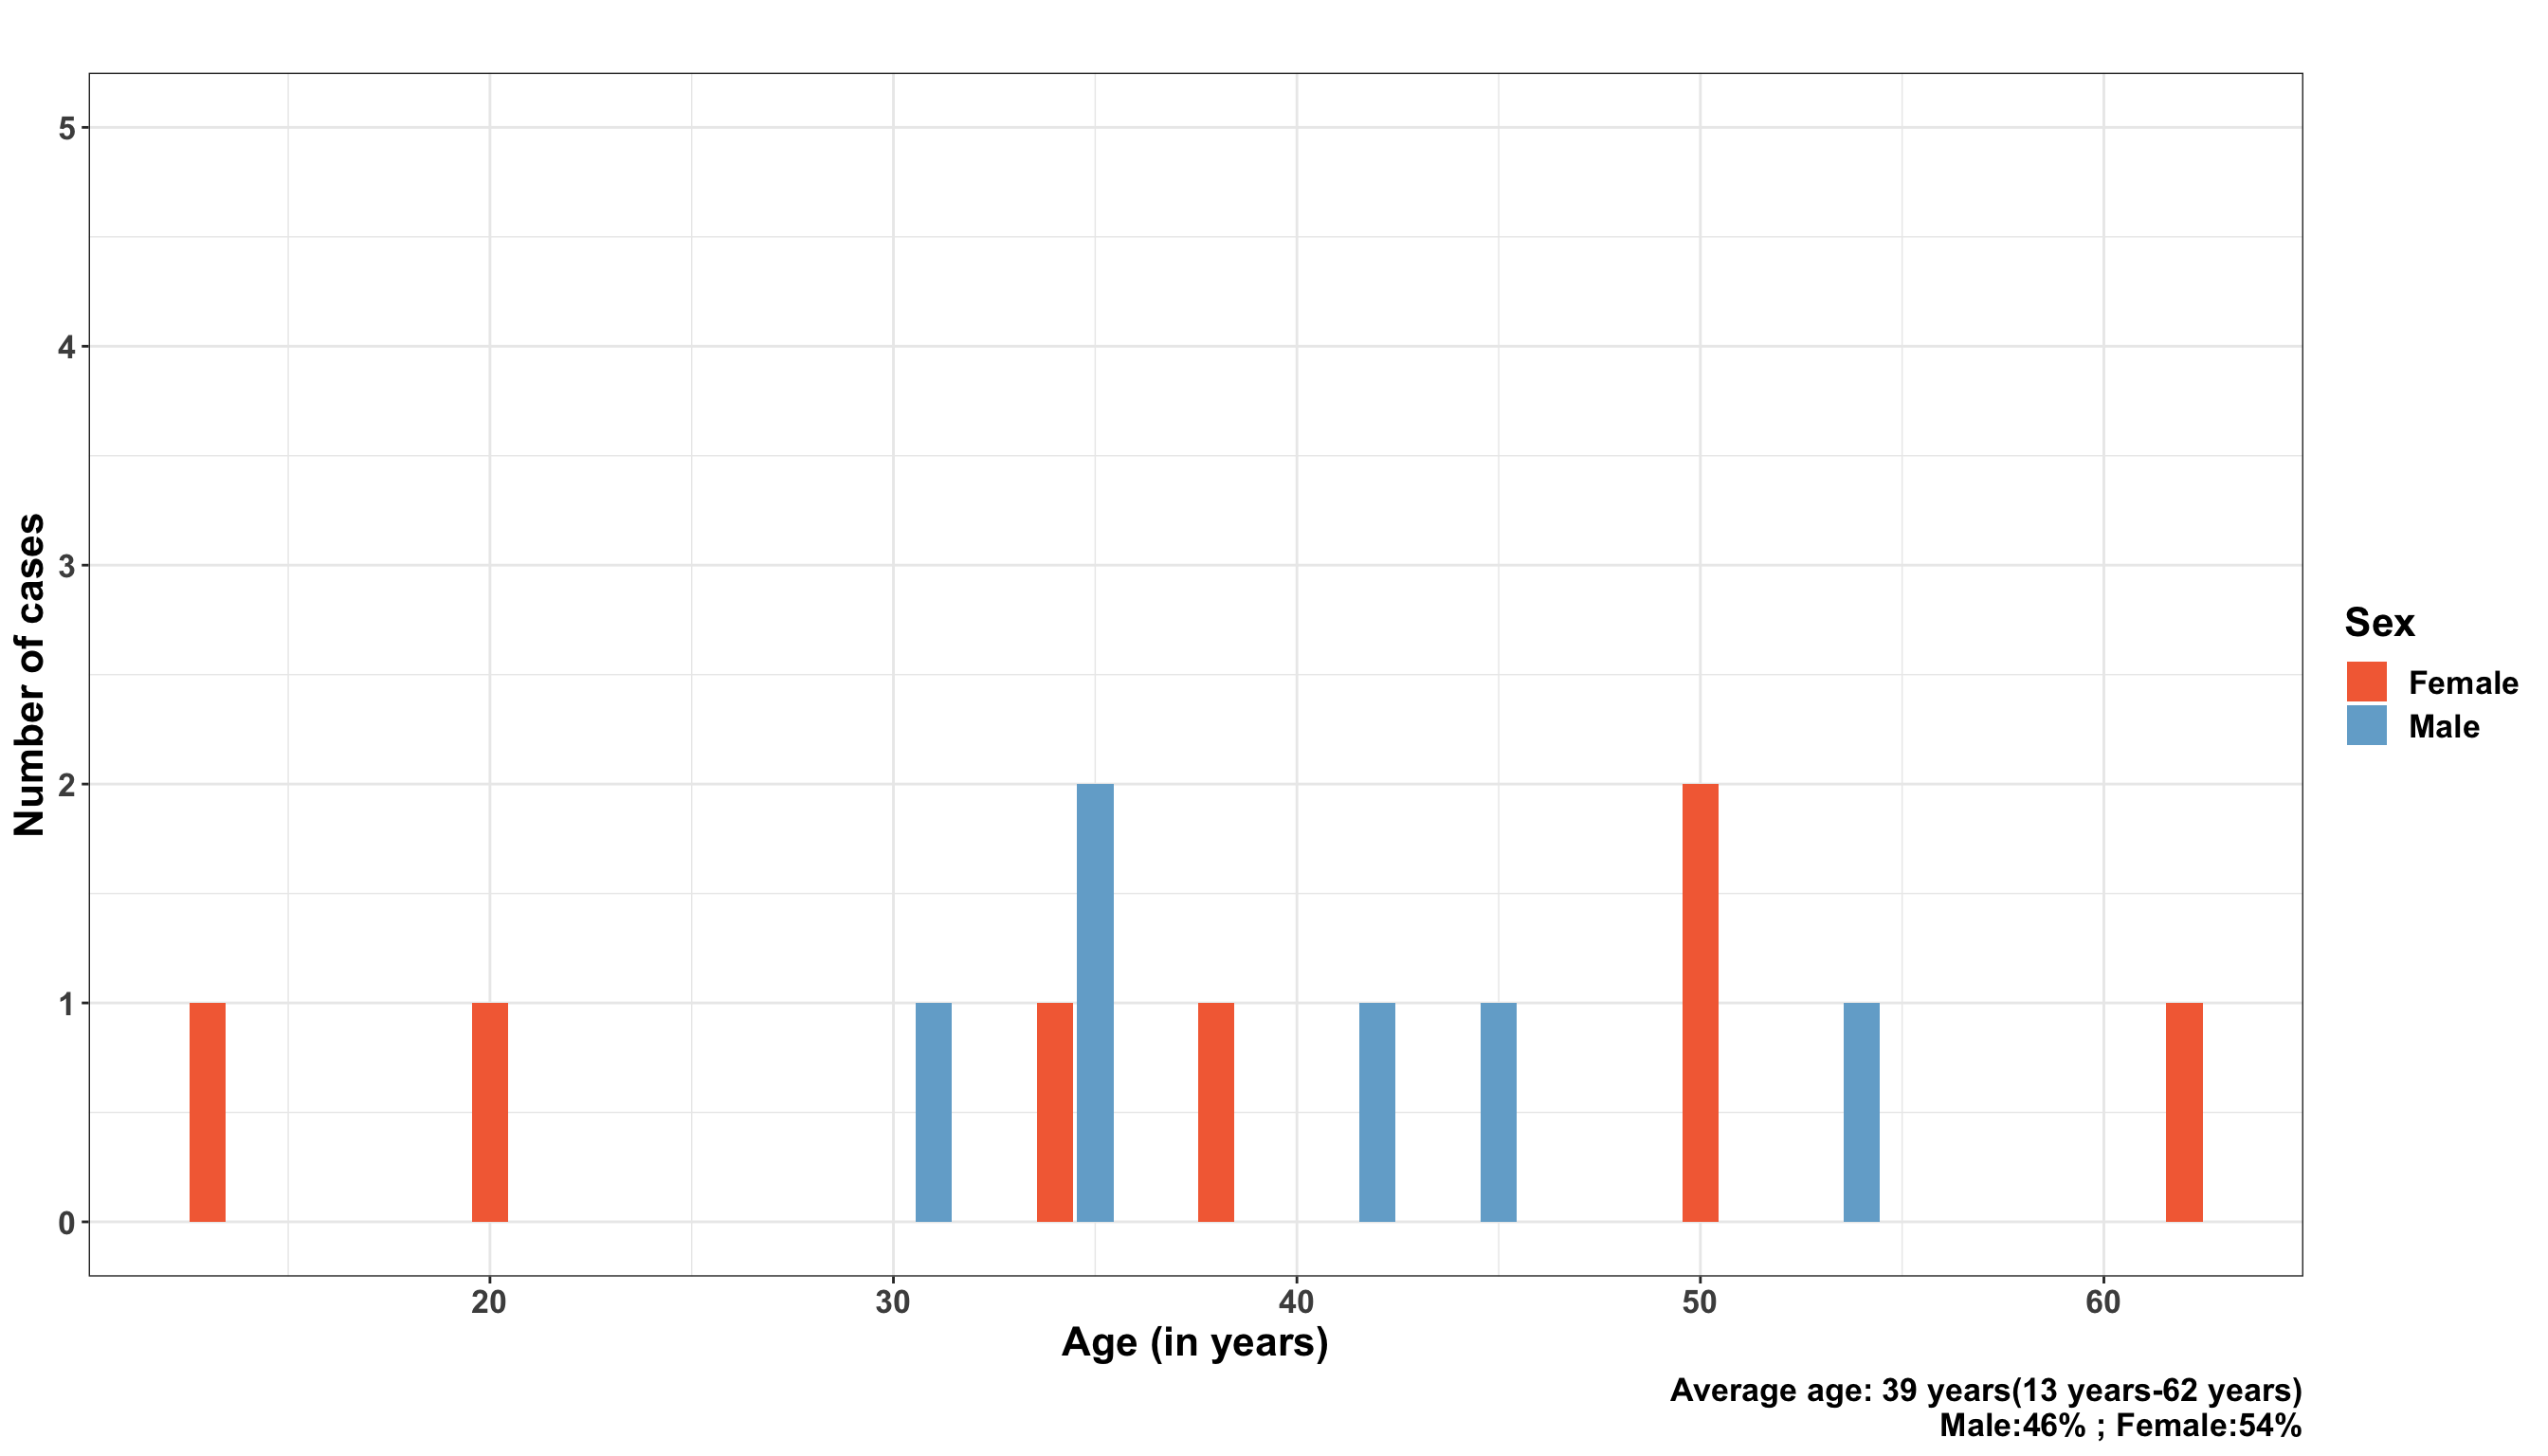
\includegraphics{_main_files/figure-latex/unnamed-chunk-78-1.pdf}

\hypertarget{spatial-distribution-12}{%
\section{Spatial distribution}\label{spatial-distribution-12}}

The spatial distribution of these cases at subcounty level is as shown:

\hypertarget{nyeri}{%
\chapter{Nyeri}\label{nyeri}}

\hypertarget{cases-over-time-13}{%
\section{Cases over time}\label{cases-over-time-13}}

As at 2023-03-23, there were 55 cases reported in Nyeri County.

This is shown in the graph below:

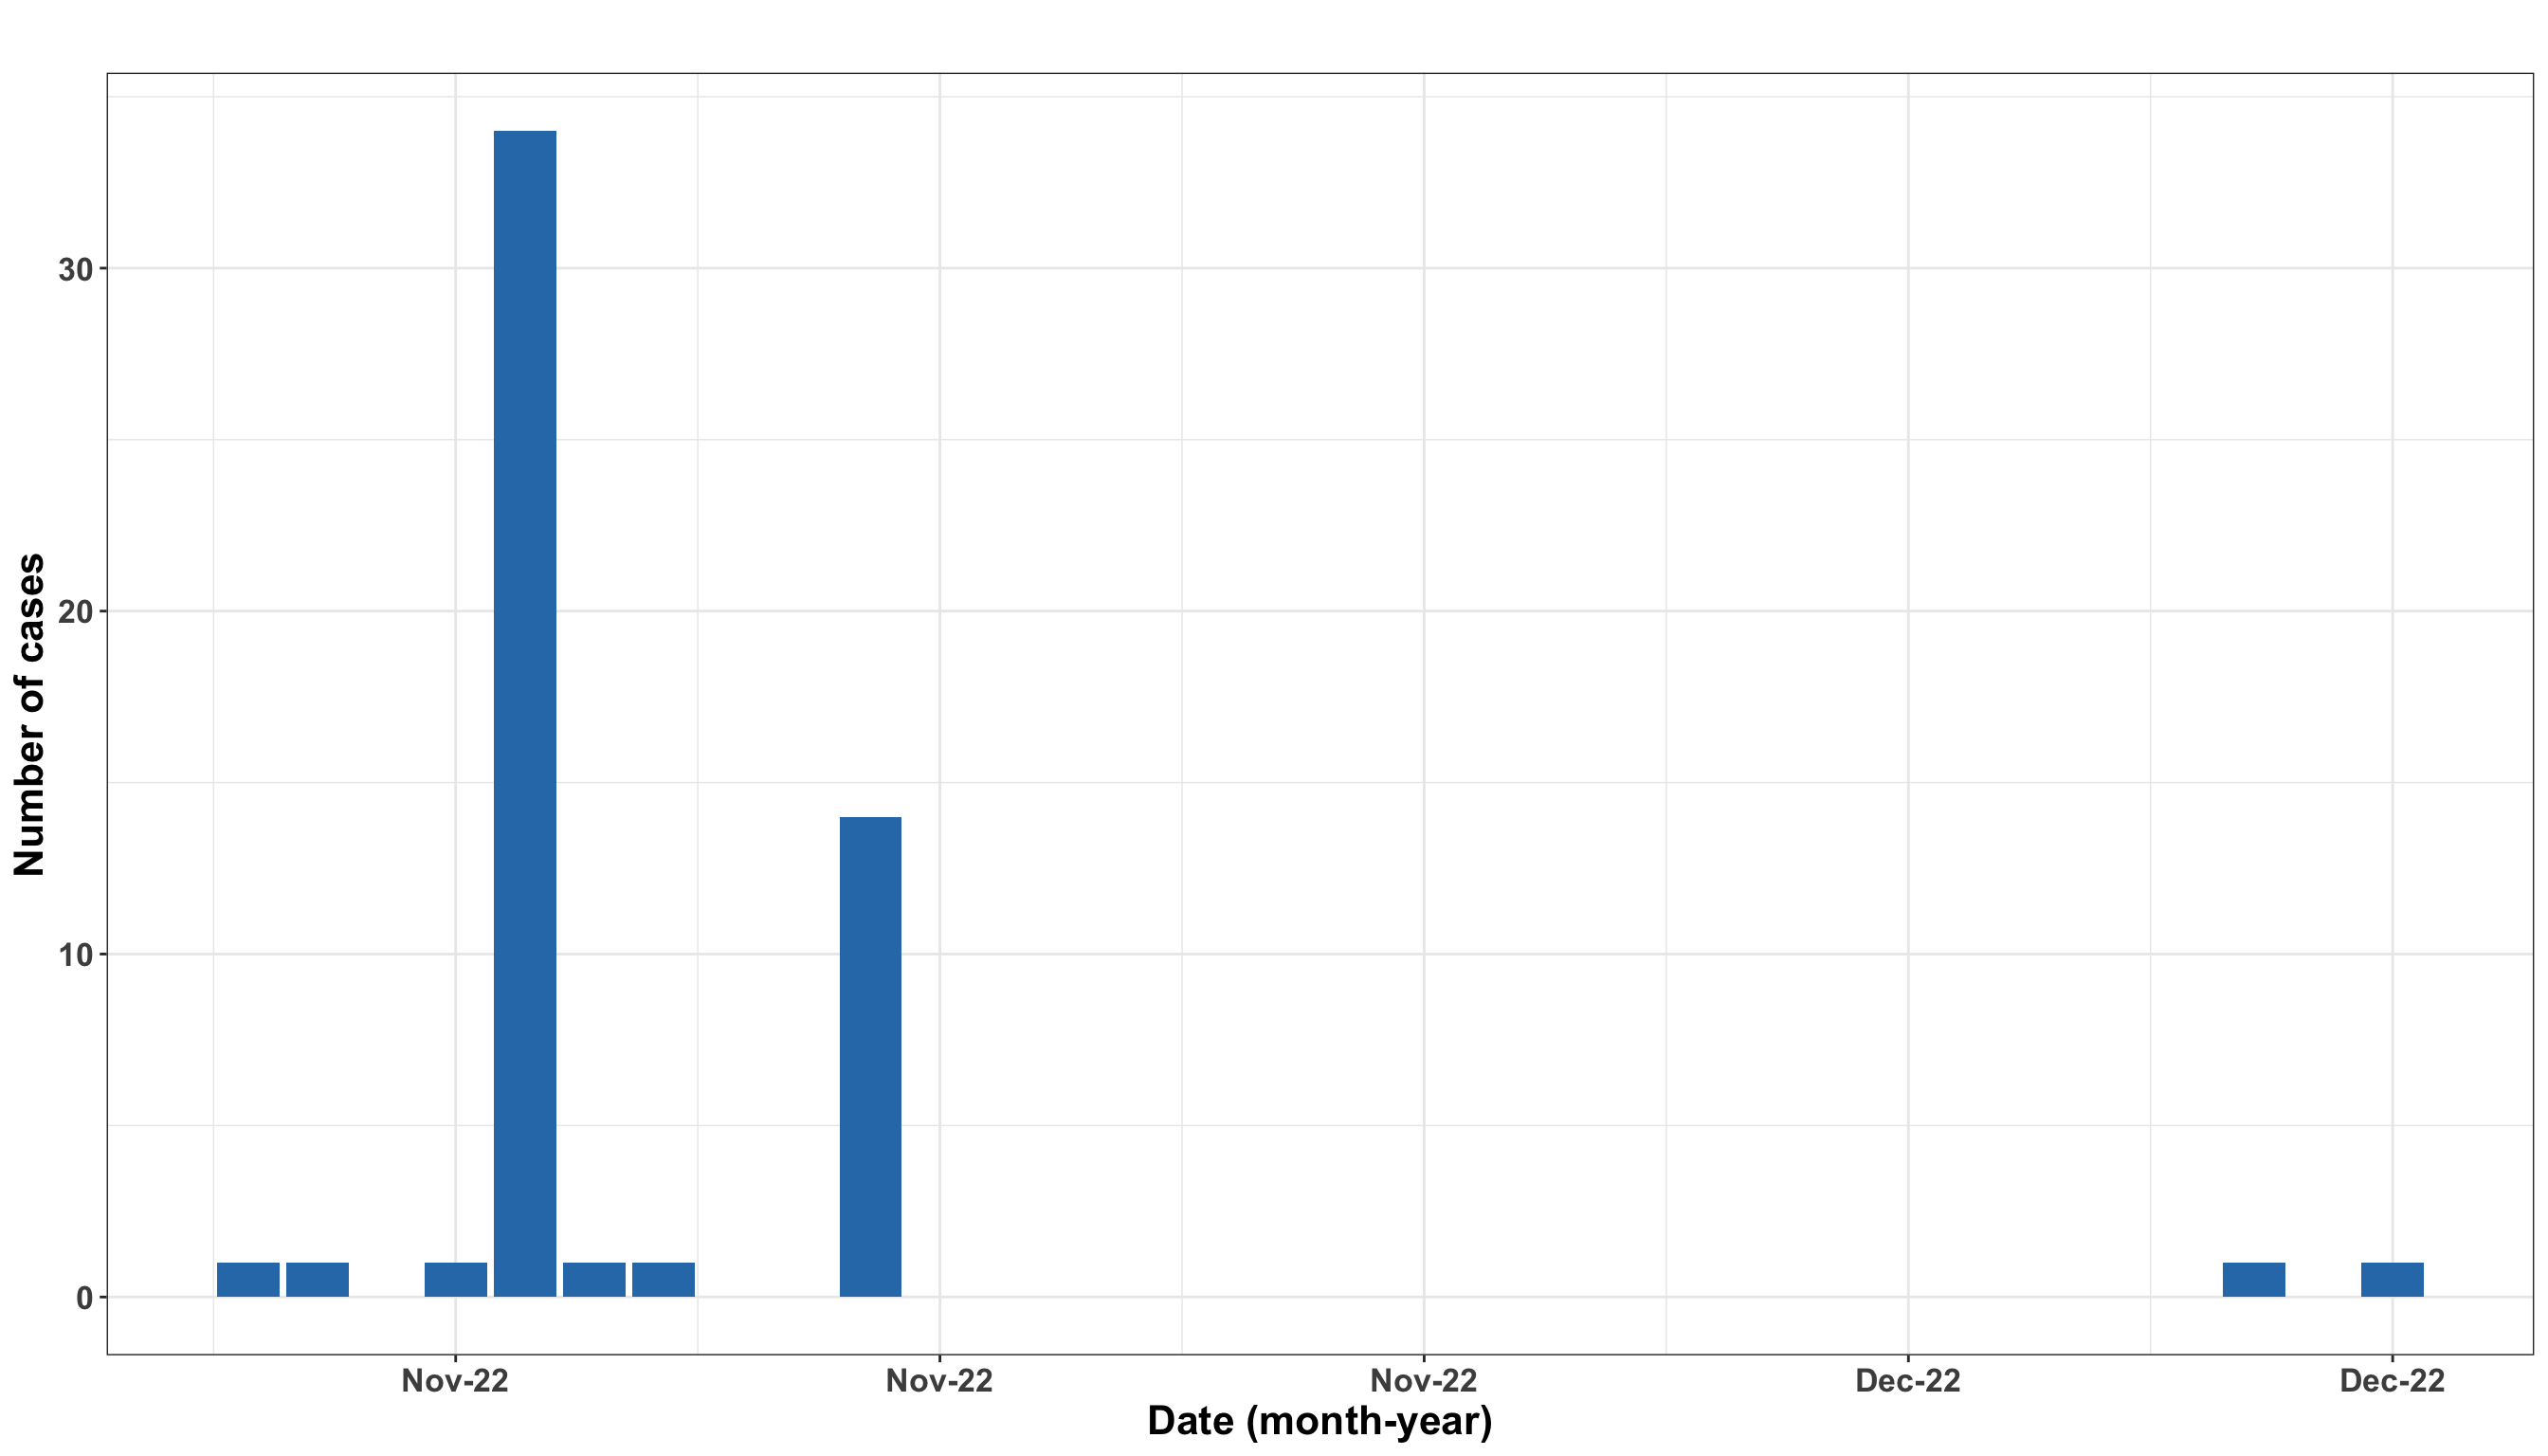
\includegraphics{_main_files/figure-latex/unnamed-chunk-82-1.pdf}

\hypertarget{demographic-distribution-13}{%
\section{Demographic distribution}\label{demographic-distribution-13}}

The stratification of these cases by age and sex is as shown:

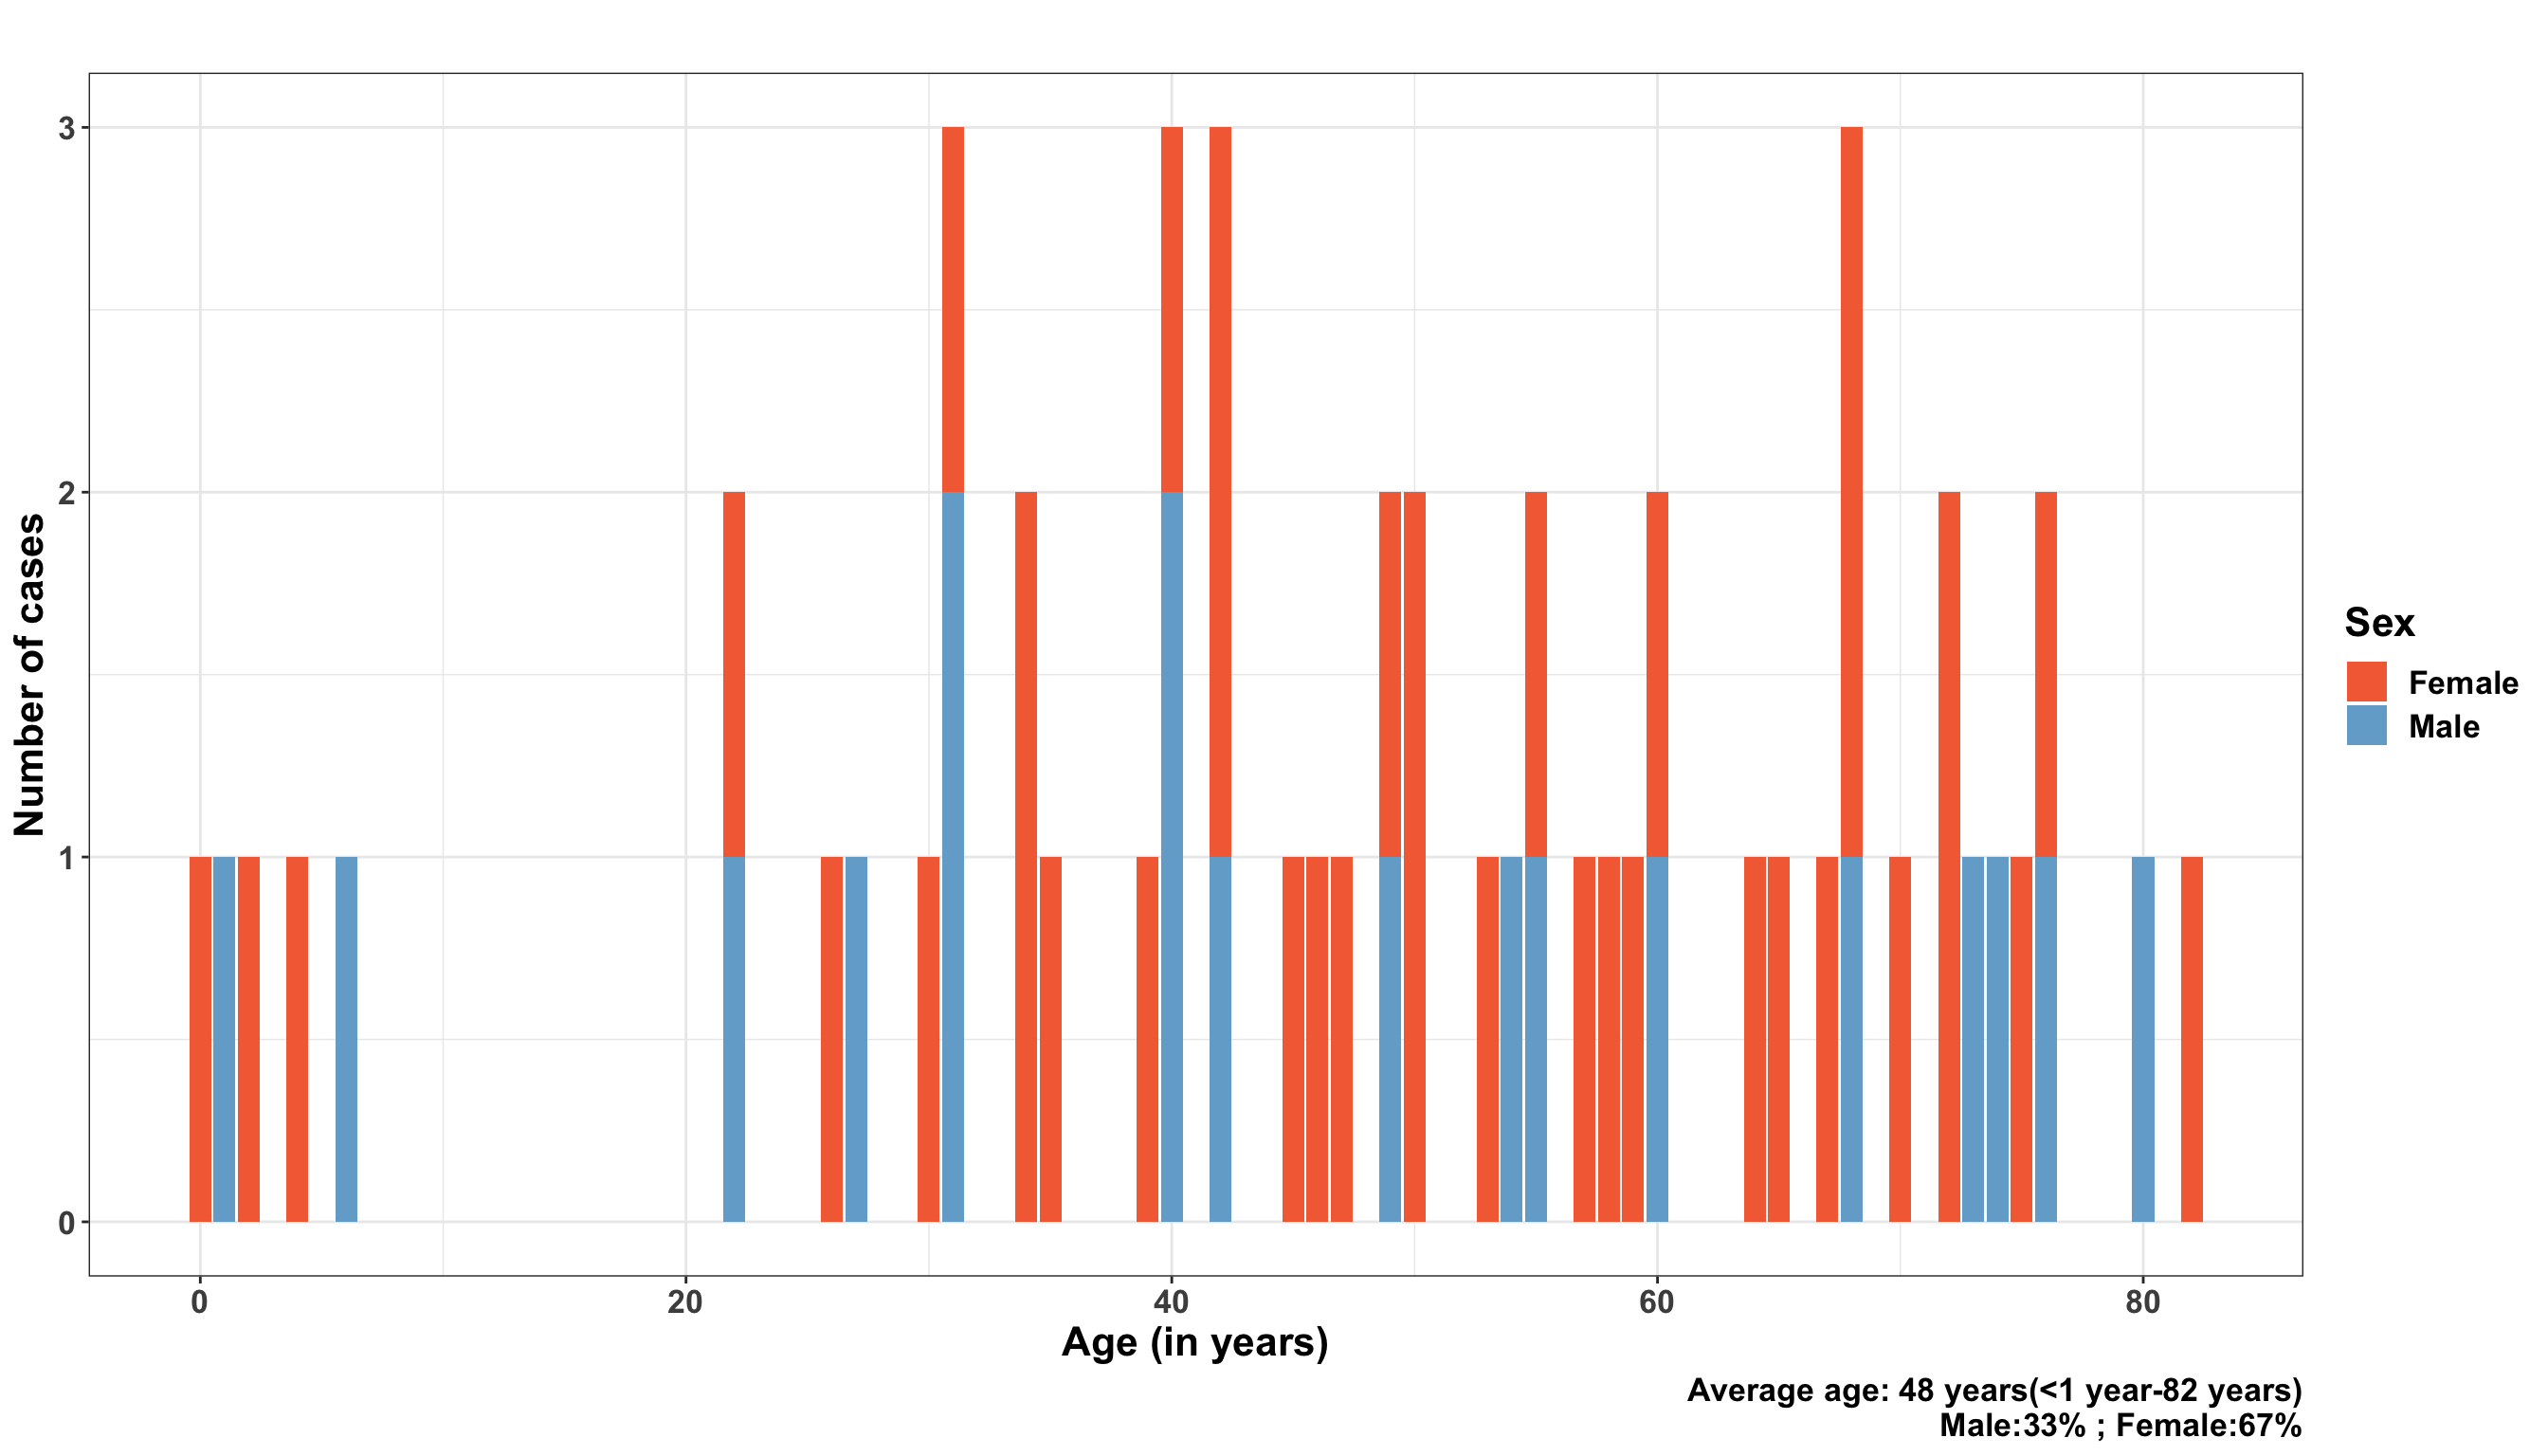
\includegraphics{_main_files/figure-latex/unnamed-chunk-84-1.pdf}

\hypertarget{spatial-distribution-13}{%
\section{Spatial distribution}\label{spatial-distribution-13}}

The spatial distribution of these cases at subcounty level is as shown:

\hypertarget{tana-river}{%
\chapter{Tana River}\label{tana-river}}

\hypertarget{cases-over-time-14}{%
\section{Cases over time}\label{cases-over-time-14}}

As at 2023-03-23, there were 762 cases reported in Tana River County.

This is shown in the graph below:

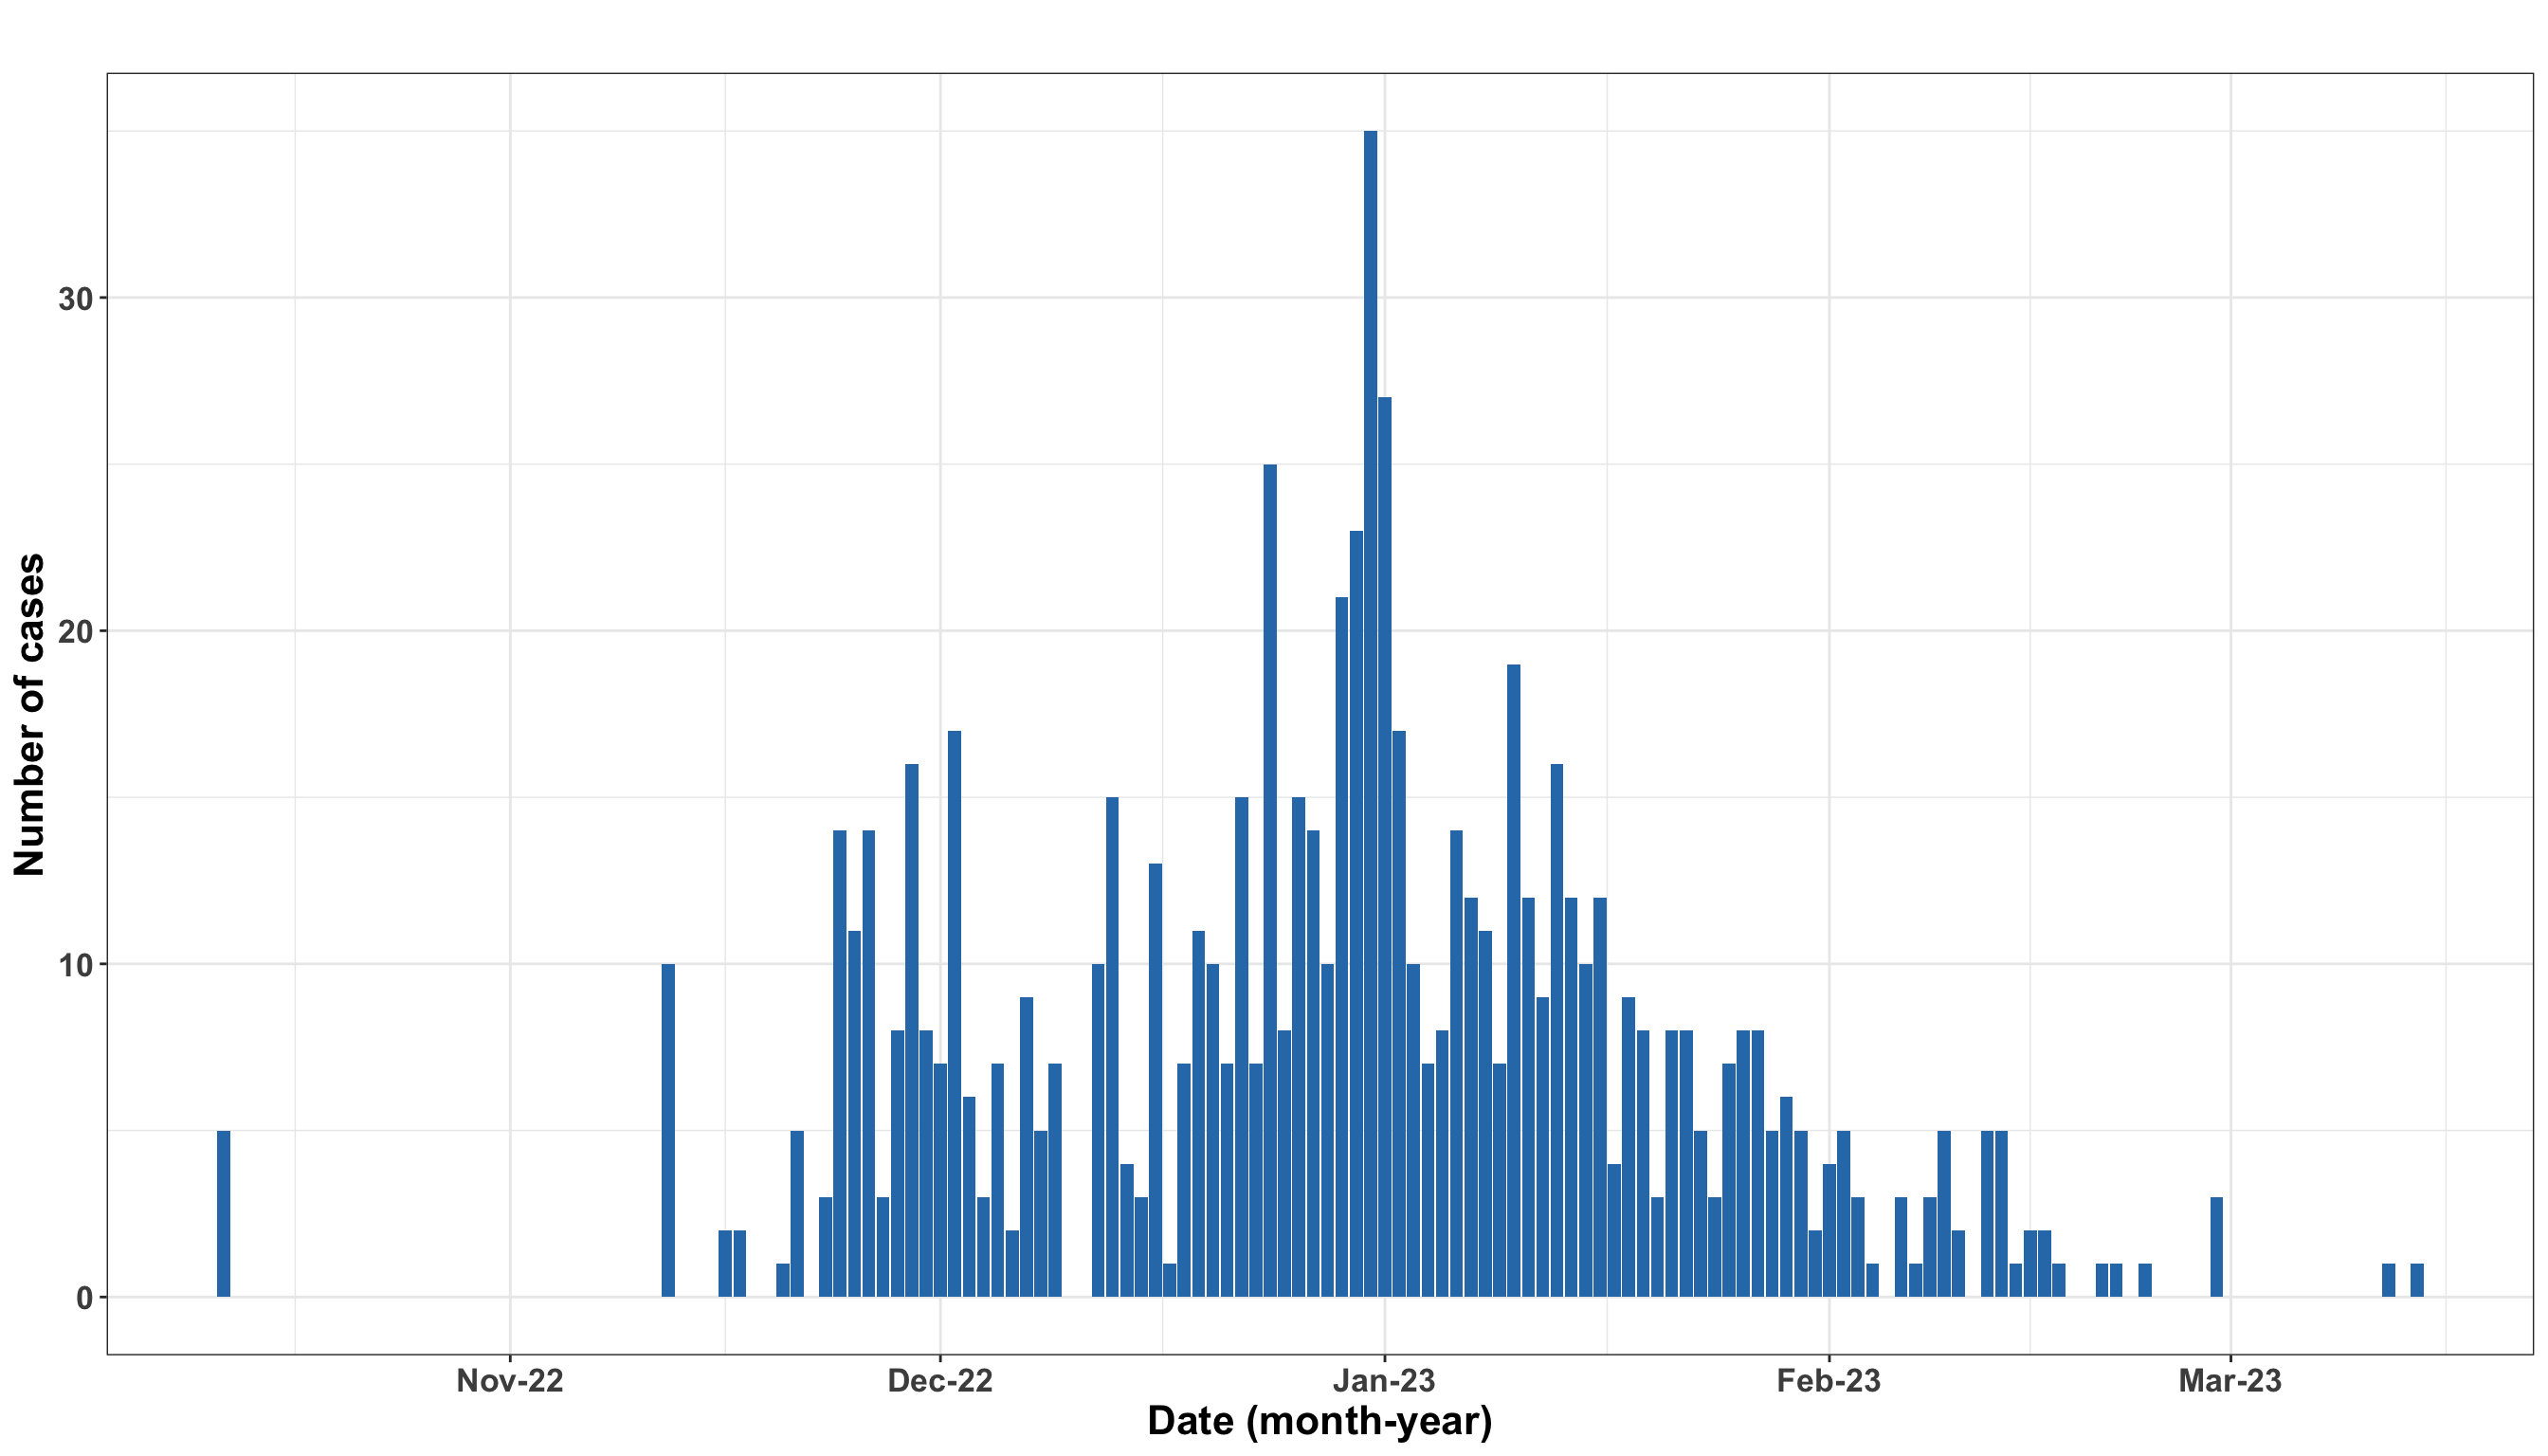
\includegraphics{_main_files/figure-latex/unnamed-chunk-88-1.pdf}

\hypertarget{demographic-distribution-14}{%
\section{Demographic distribution}\label{demographic-distribution-14}}

The stratification of these cases by age and sex is as shown:

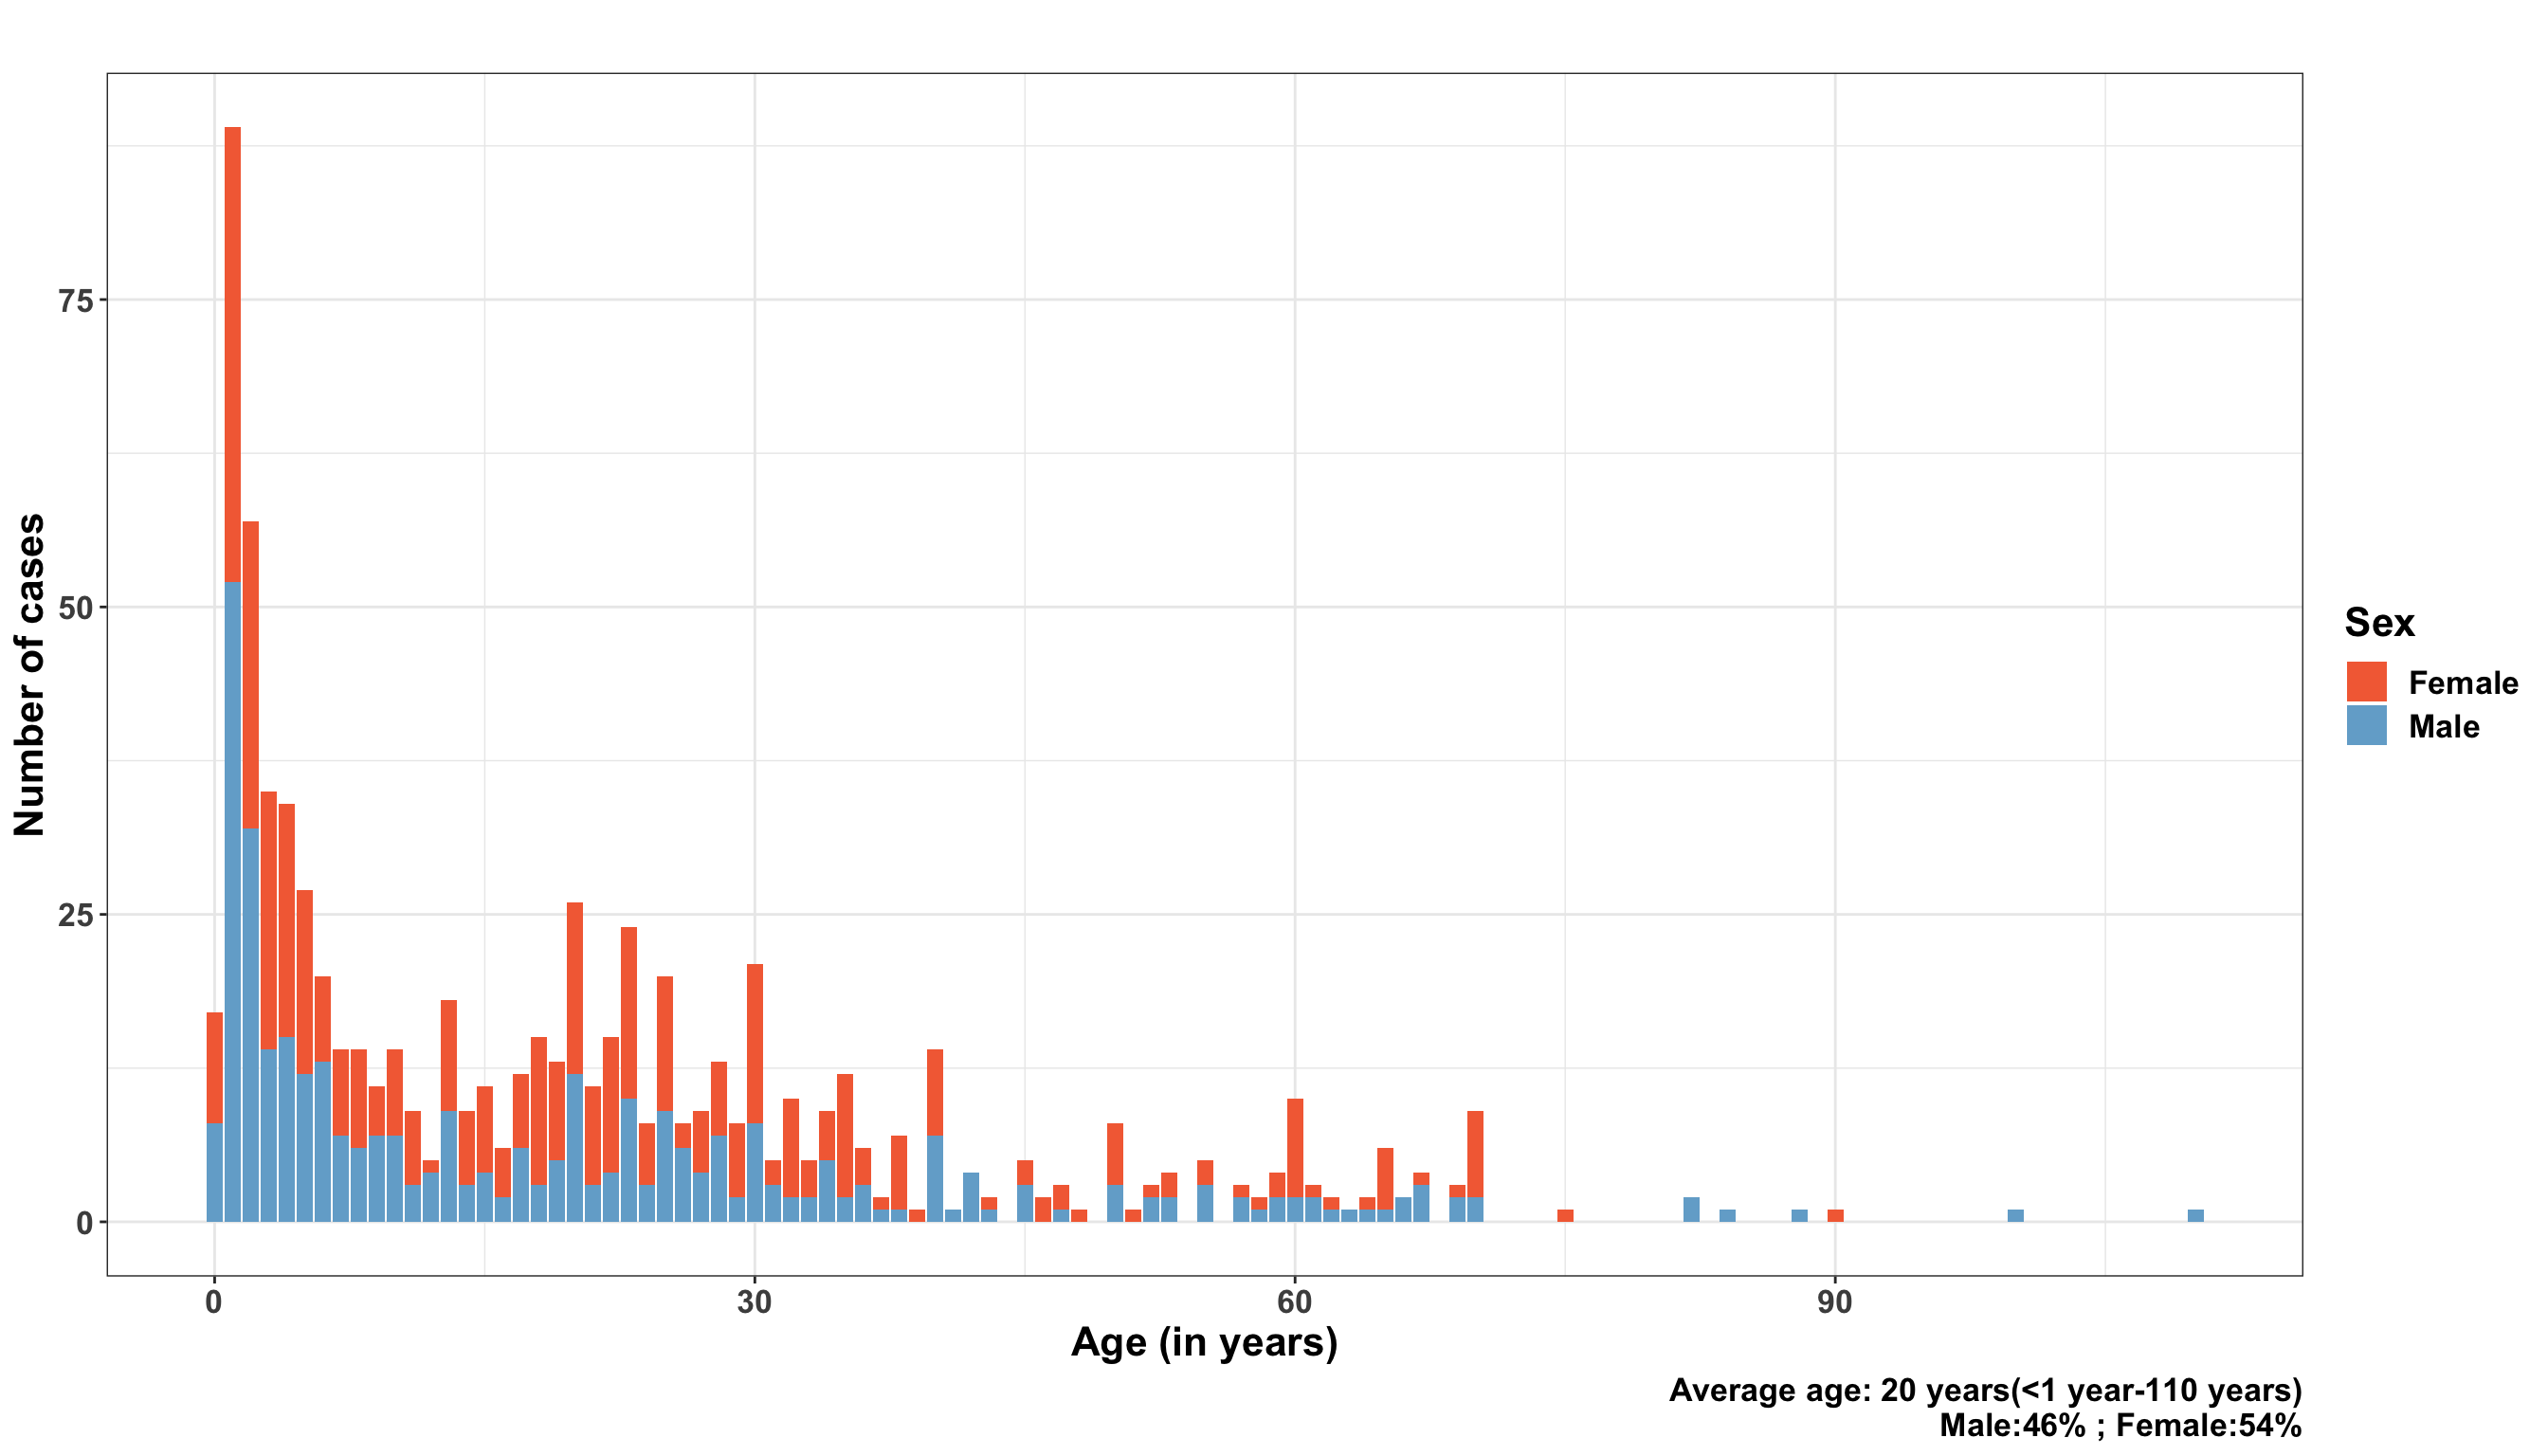
\includegraphics{_main_files/figure-latex/unnamed-chunk-90-1.pdf}

\hypertarget{spatial-distribution-14}{%
\section{Spatial distribution}\label{spatial-distribution-14}}

The spatial distribution of these cases at subcounty level is as shown:

\hypertarget{uasin-gishu}{%
\chapter{Uasin Gishu}\label{uasin-gishu}}

\hypertarget{cases-over-time-15}{%
\section{Cases over time}\label{cases-over-time-15}}

As at 2023-03-23, there were 8 cases reported in Uasin Gishu County.

This is shown in the graph below:

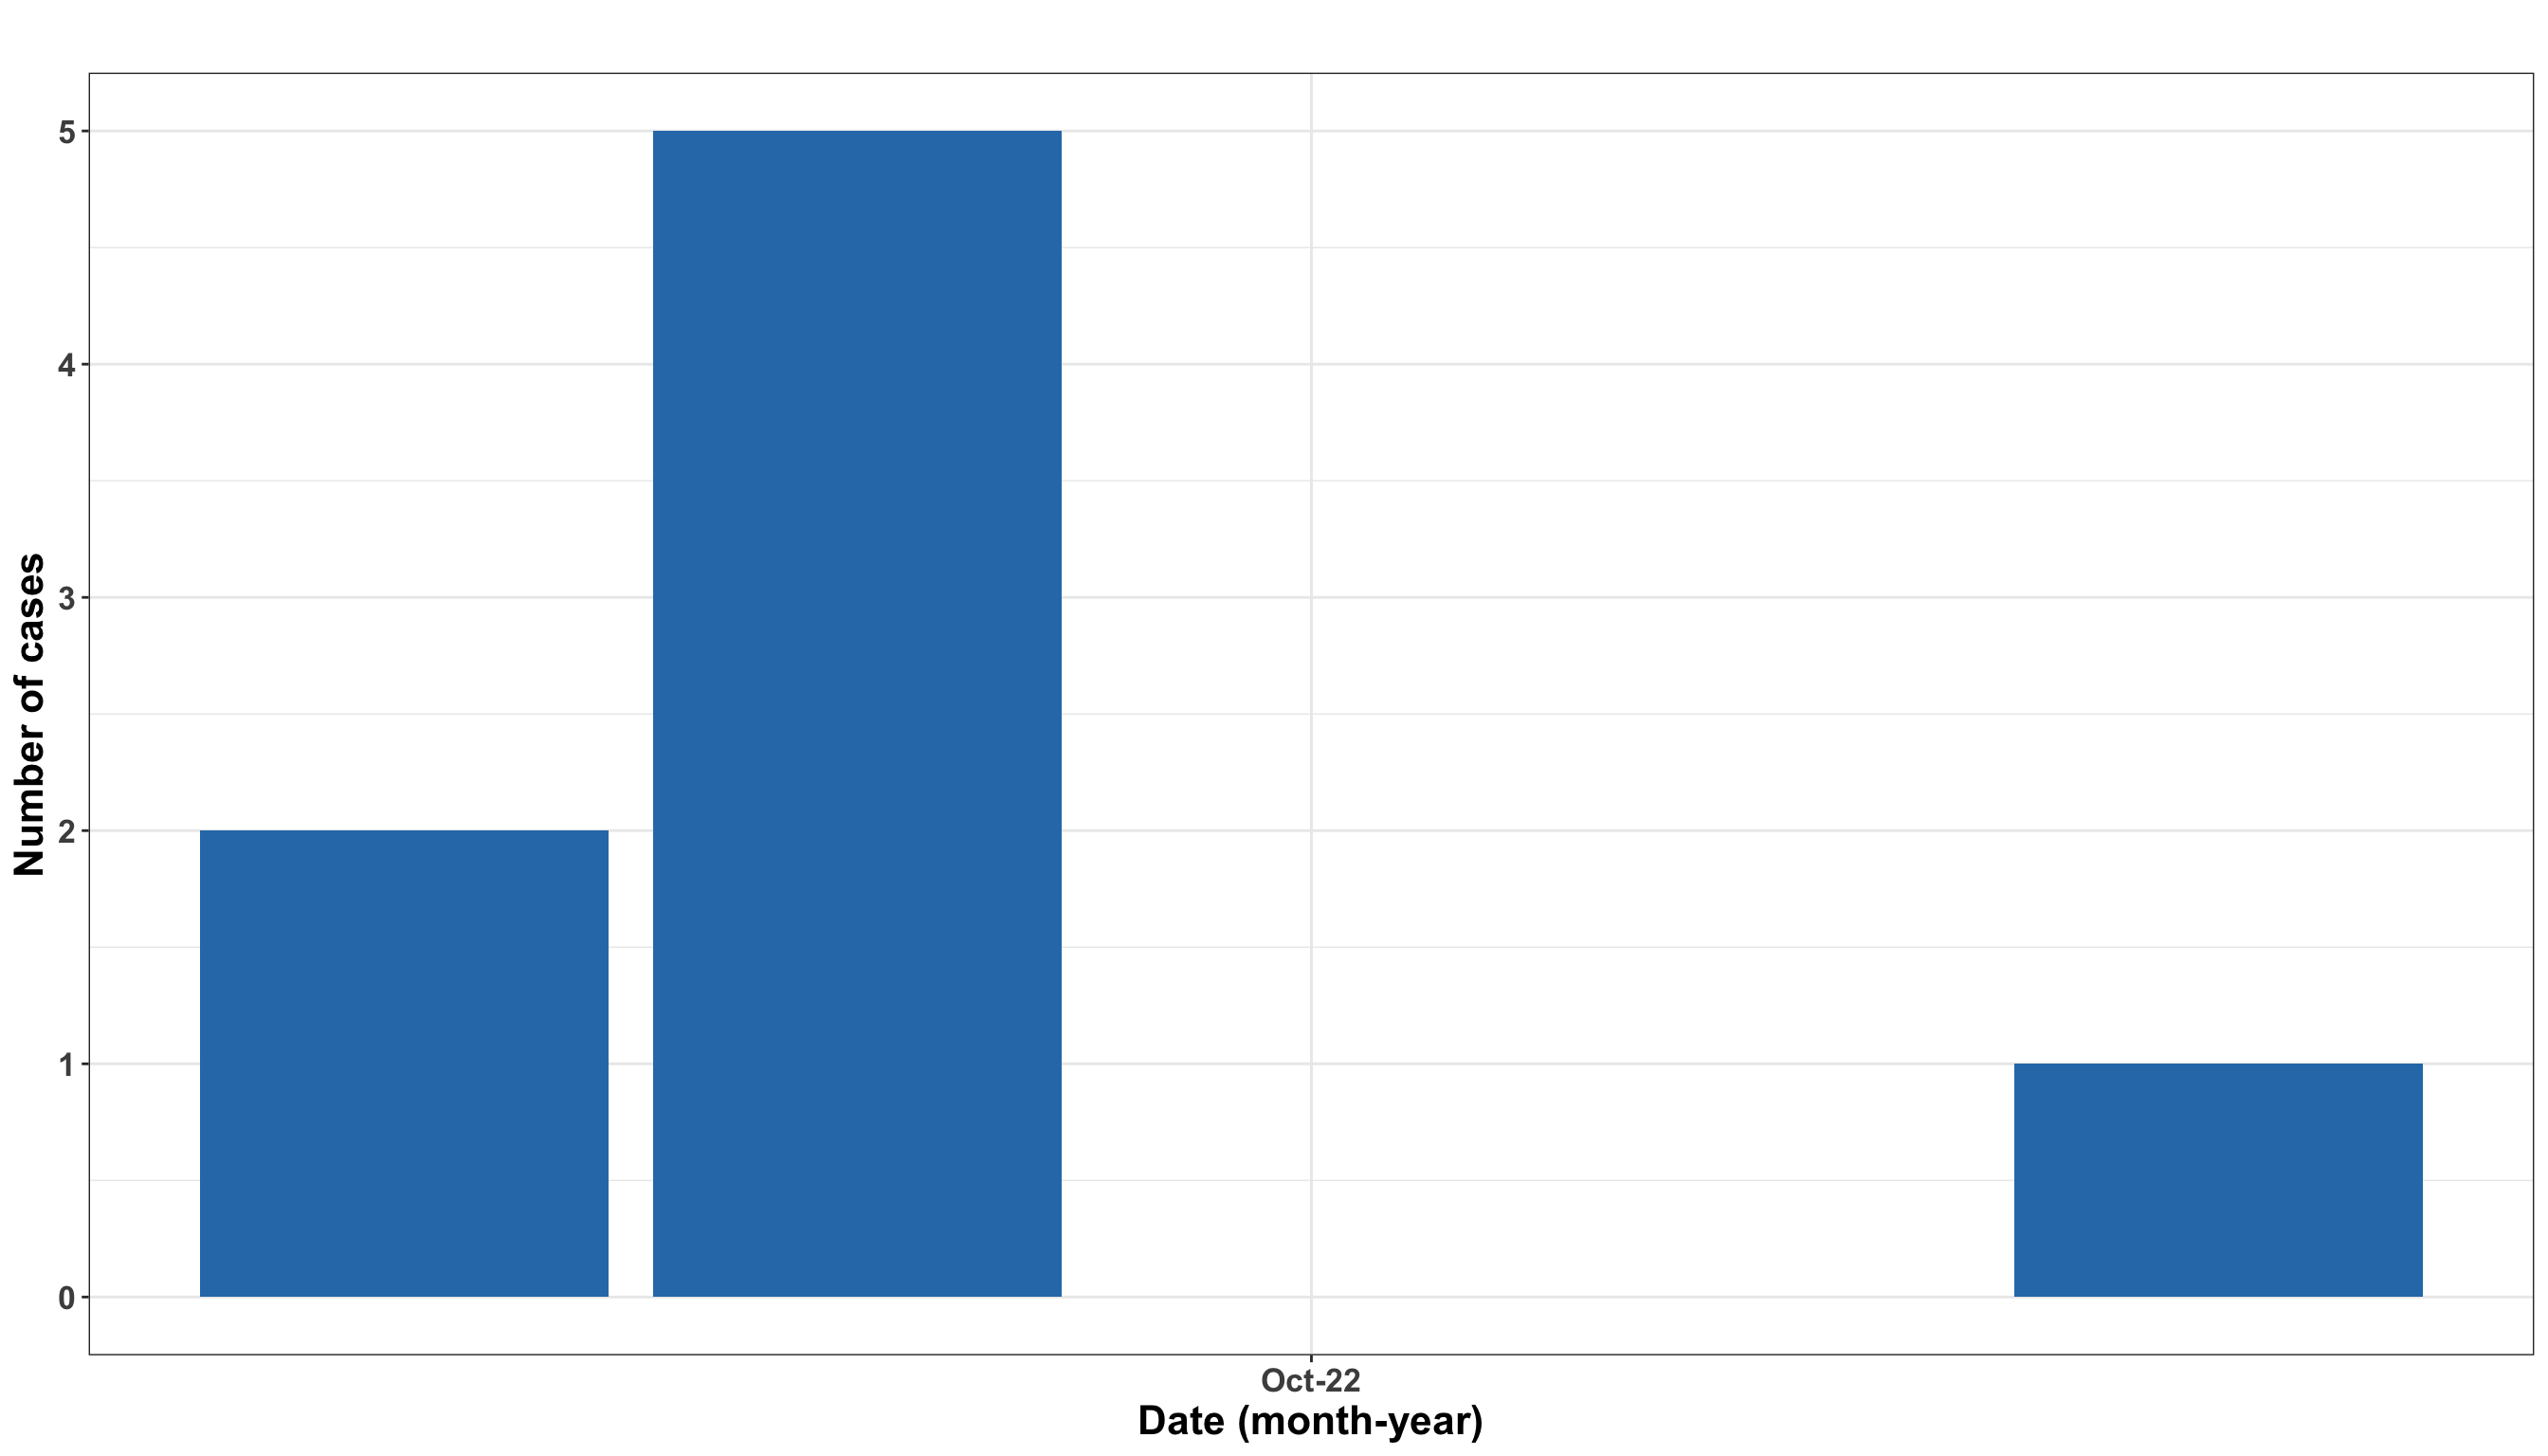
\includegraphics{_main_files/figure-latex/unnamed-chunk-94-1.pdf}

\hypertarget{demographic-distribution-15}{%
\section{Demographic distribution}\label{demographic-distribution-15}}

The stratification of these cases by age and sex is as shown:

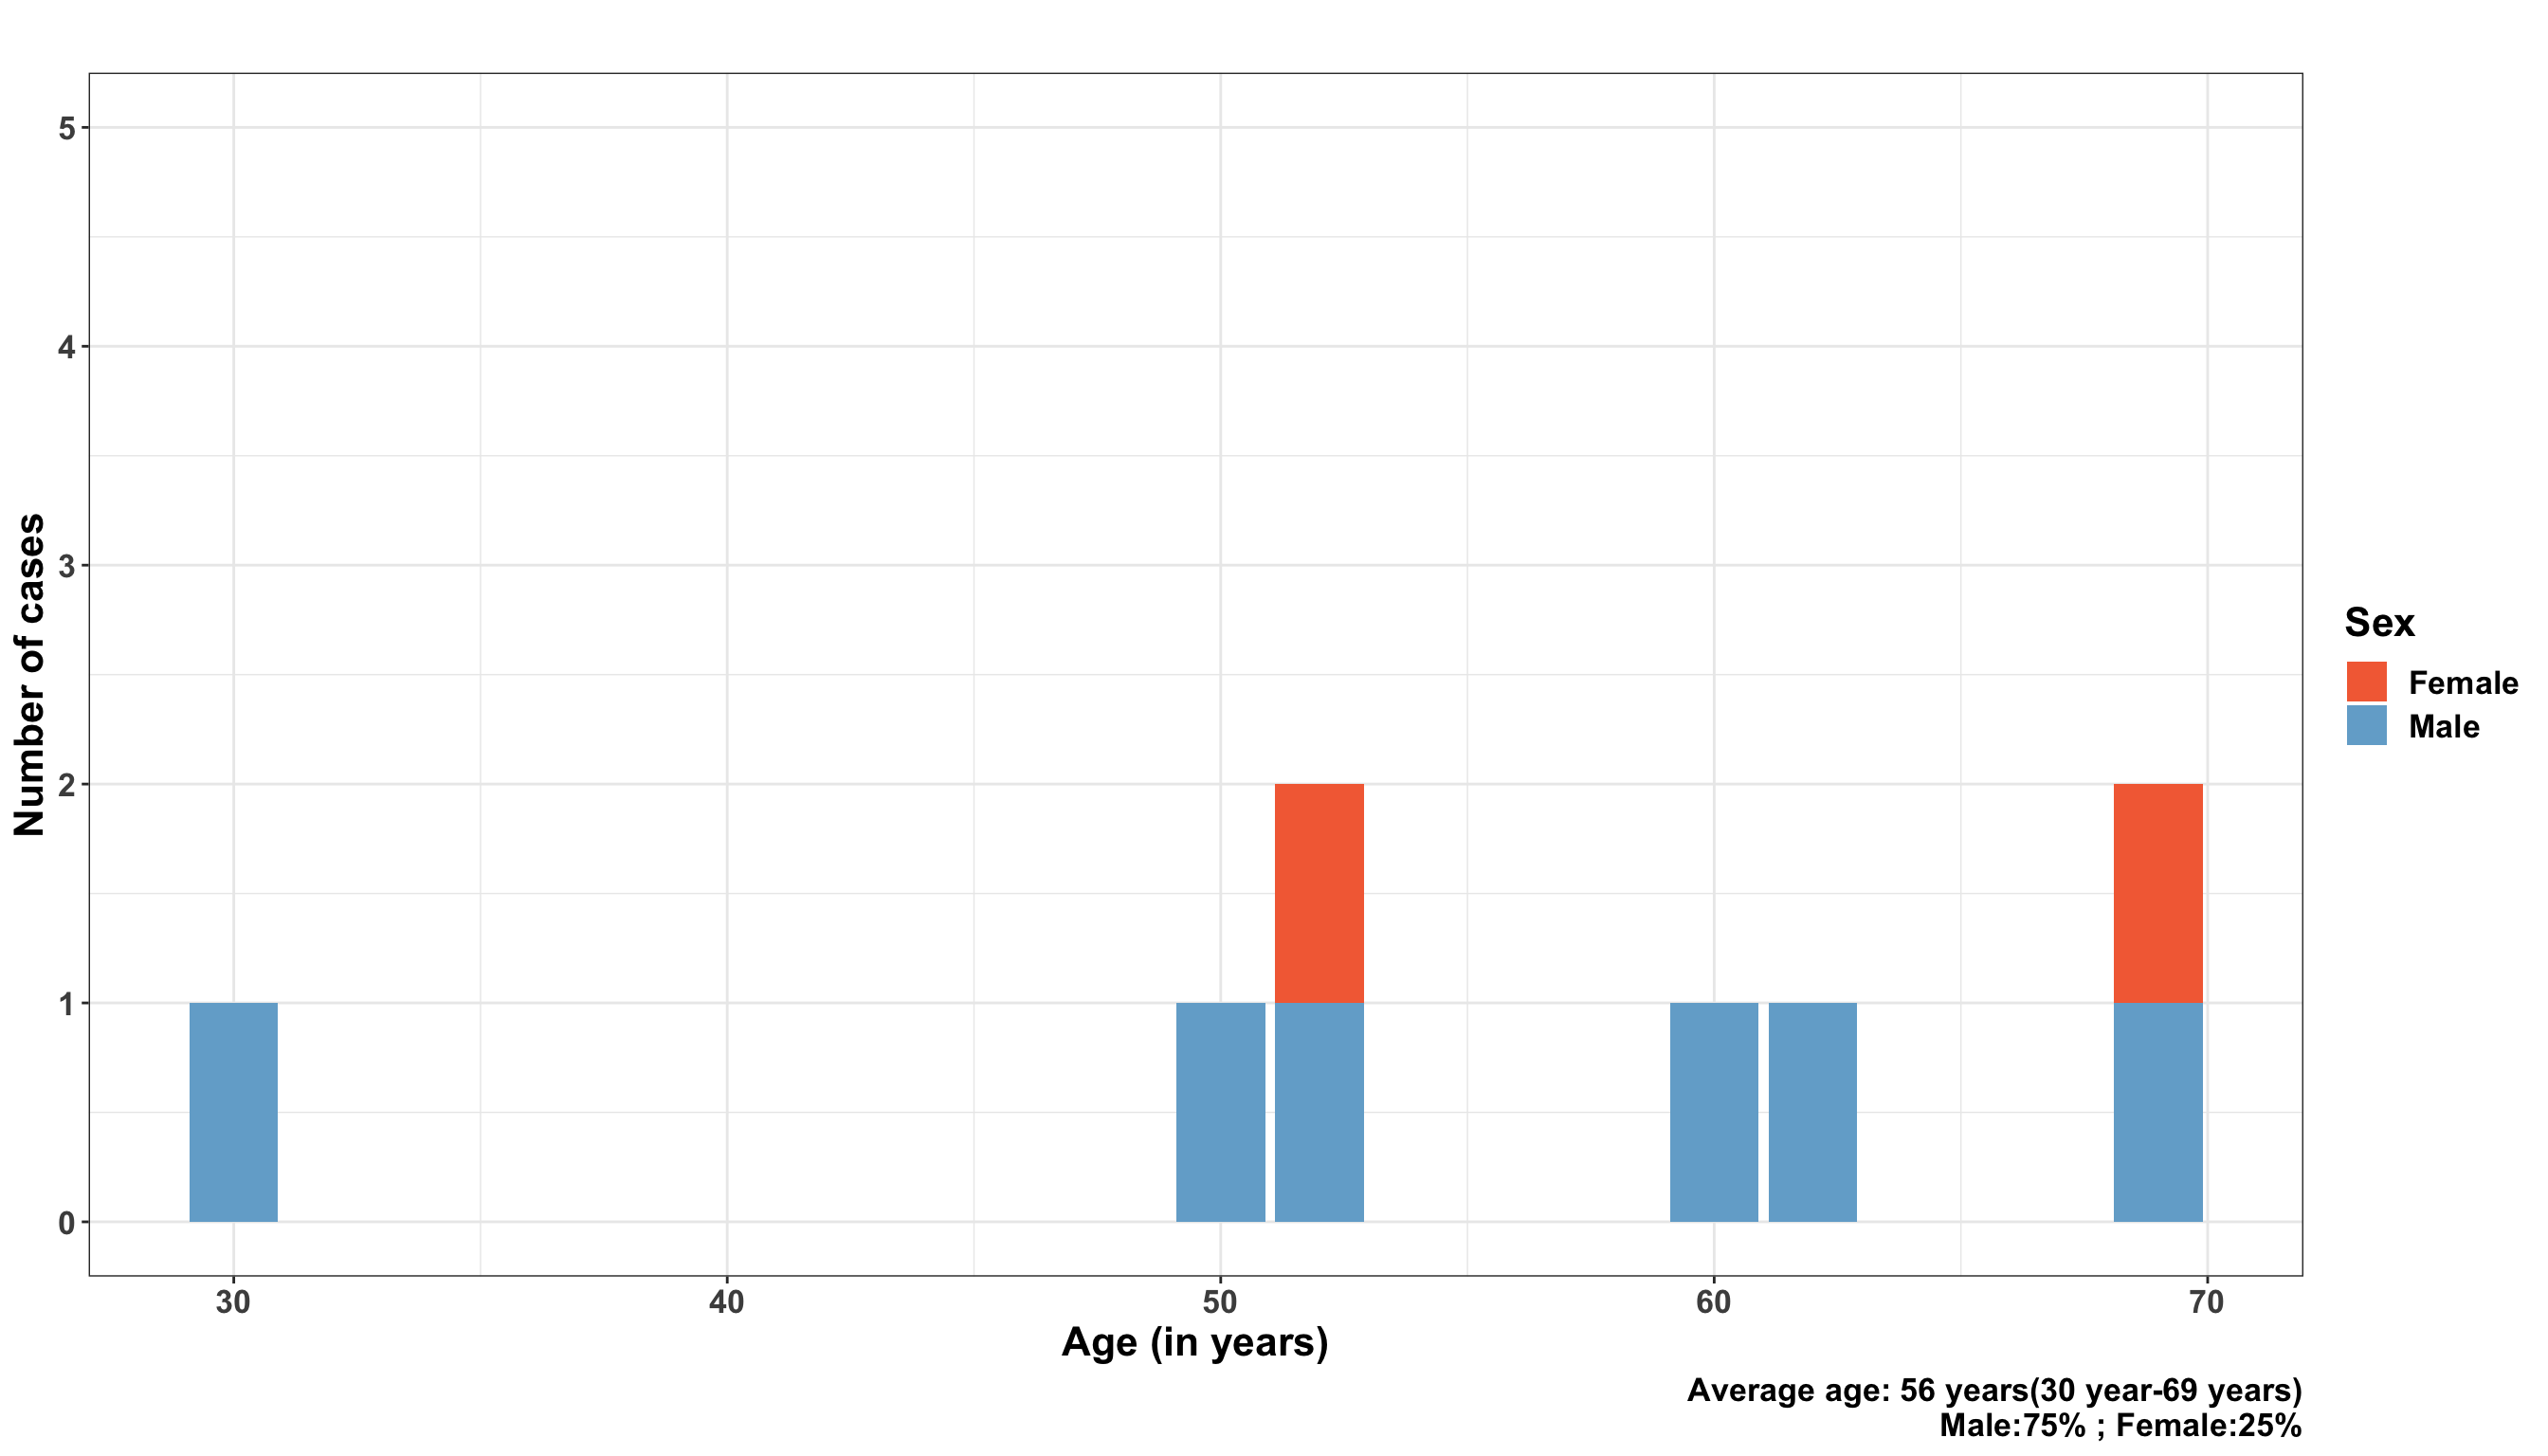
\includegraphics{_main_files/figure-latex/unnamed-chunk-96-1.pdf}

\hypertarget{spatial-distribution-15}{%
\section{Spatial distribution}\label{spatial-distribution-15}}

The spatial distribution of these cases at subcounty level is as shown:

\hypertarget{wajir}{%
\chapter{Wajir}\label{wajir}}

\hypertarget{cases-over-time-16}{%
\section{Cases over time}\label{cases-over-time-16}}

As at 2023-03-23, there were 654 cases reported in Wajir County.

This is shown in the graph below:

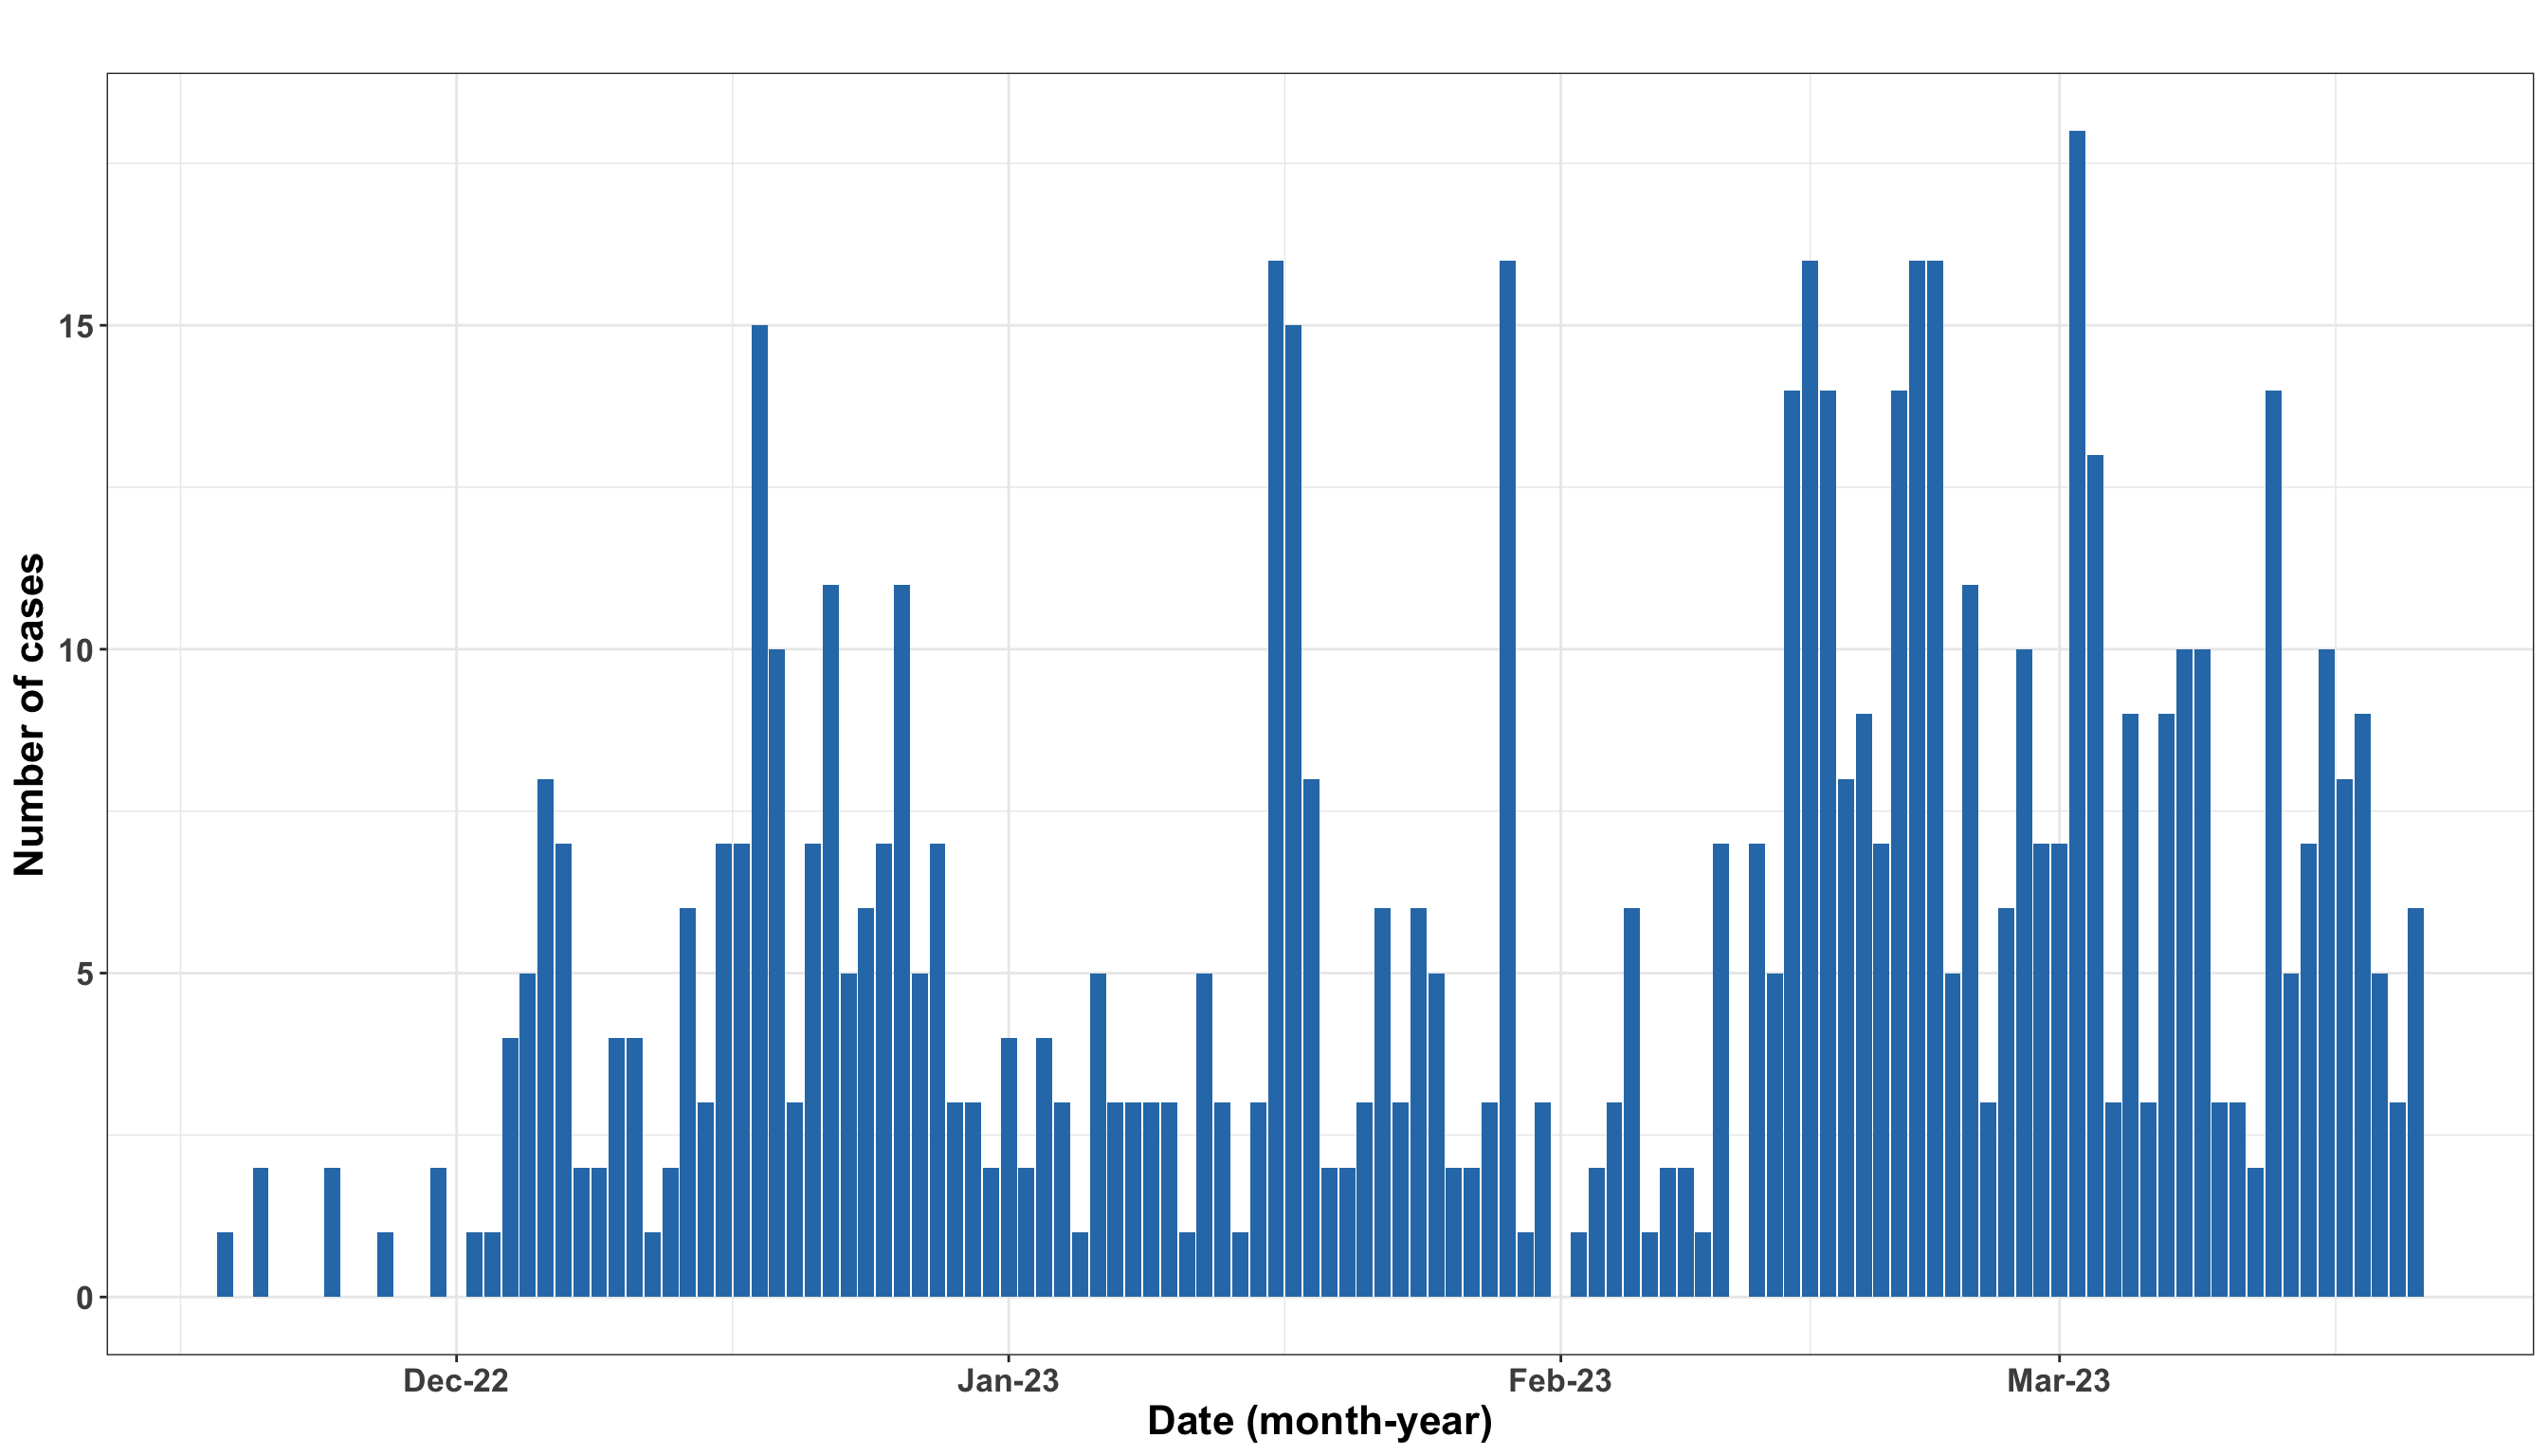
\includegraphics{_main_files/figure-latex/unnamed-chunk-100-1.pdf}

\hypertarget{demographic-distribution-16}{%
\section{Demographic distribution}\label{demographic-distribution-16}}

The stratification of these cases by age and sex is as shown:

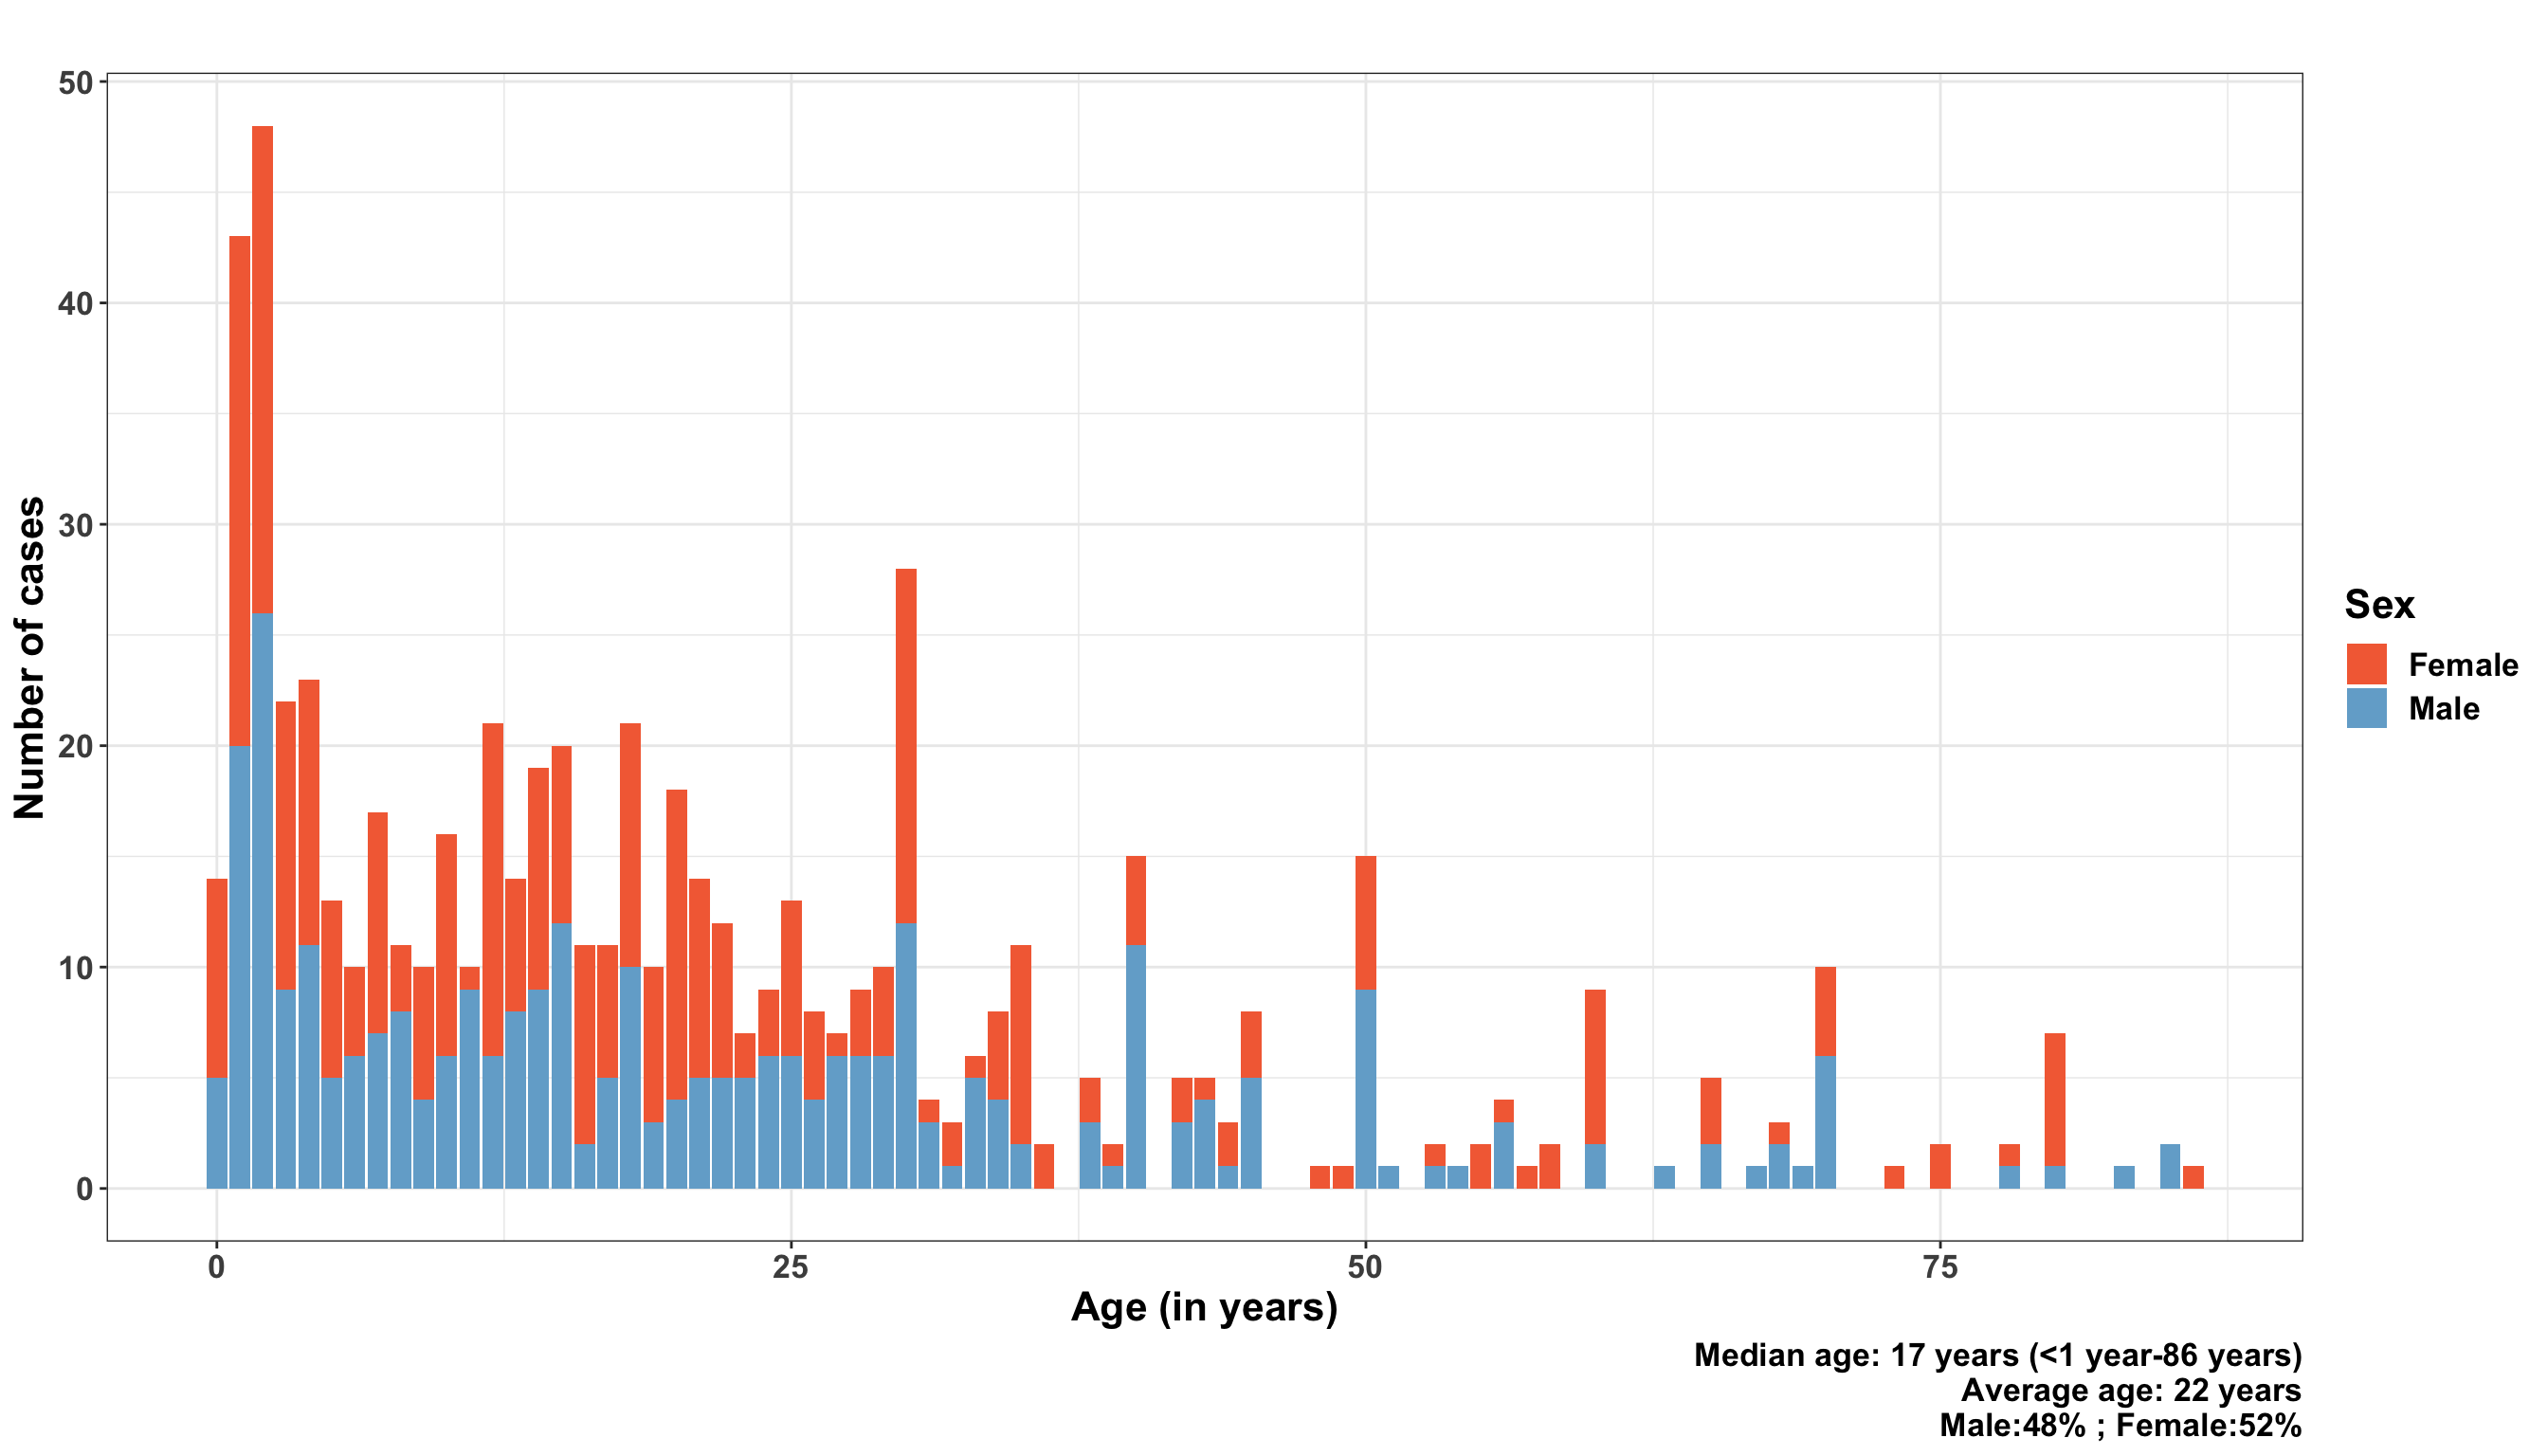
\includegraphics{_main_files/figure-latex/unnamed-chunk-102-1.pdf}

\hypertarget{spatial-distribution-16}{%
\section{Spatial distribution}\label{spatial-distribution-16}}

The spatial distribution of these cases at subcounty level is as shown:

\hypertarget{west-pokot}{%
\chapter{West Pokot}\label{west-pokot}}

\hypertarget{cases-over-time-17}{%
\section{Cases over time}\label{cases-over-time-17}}

As at 2023-03-23, there were 16 cases reported in West Pokot County.

This is shown in the graph below:

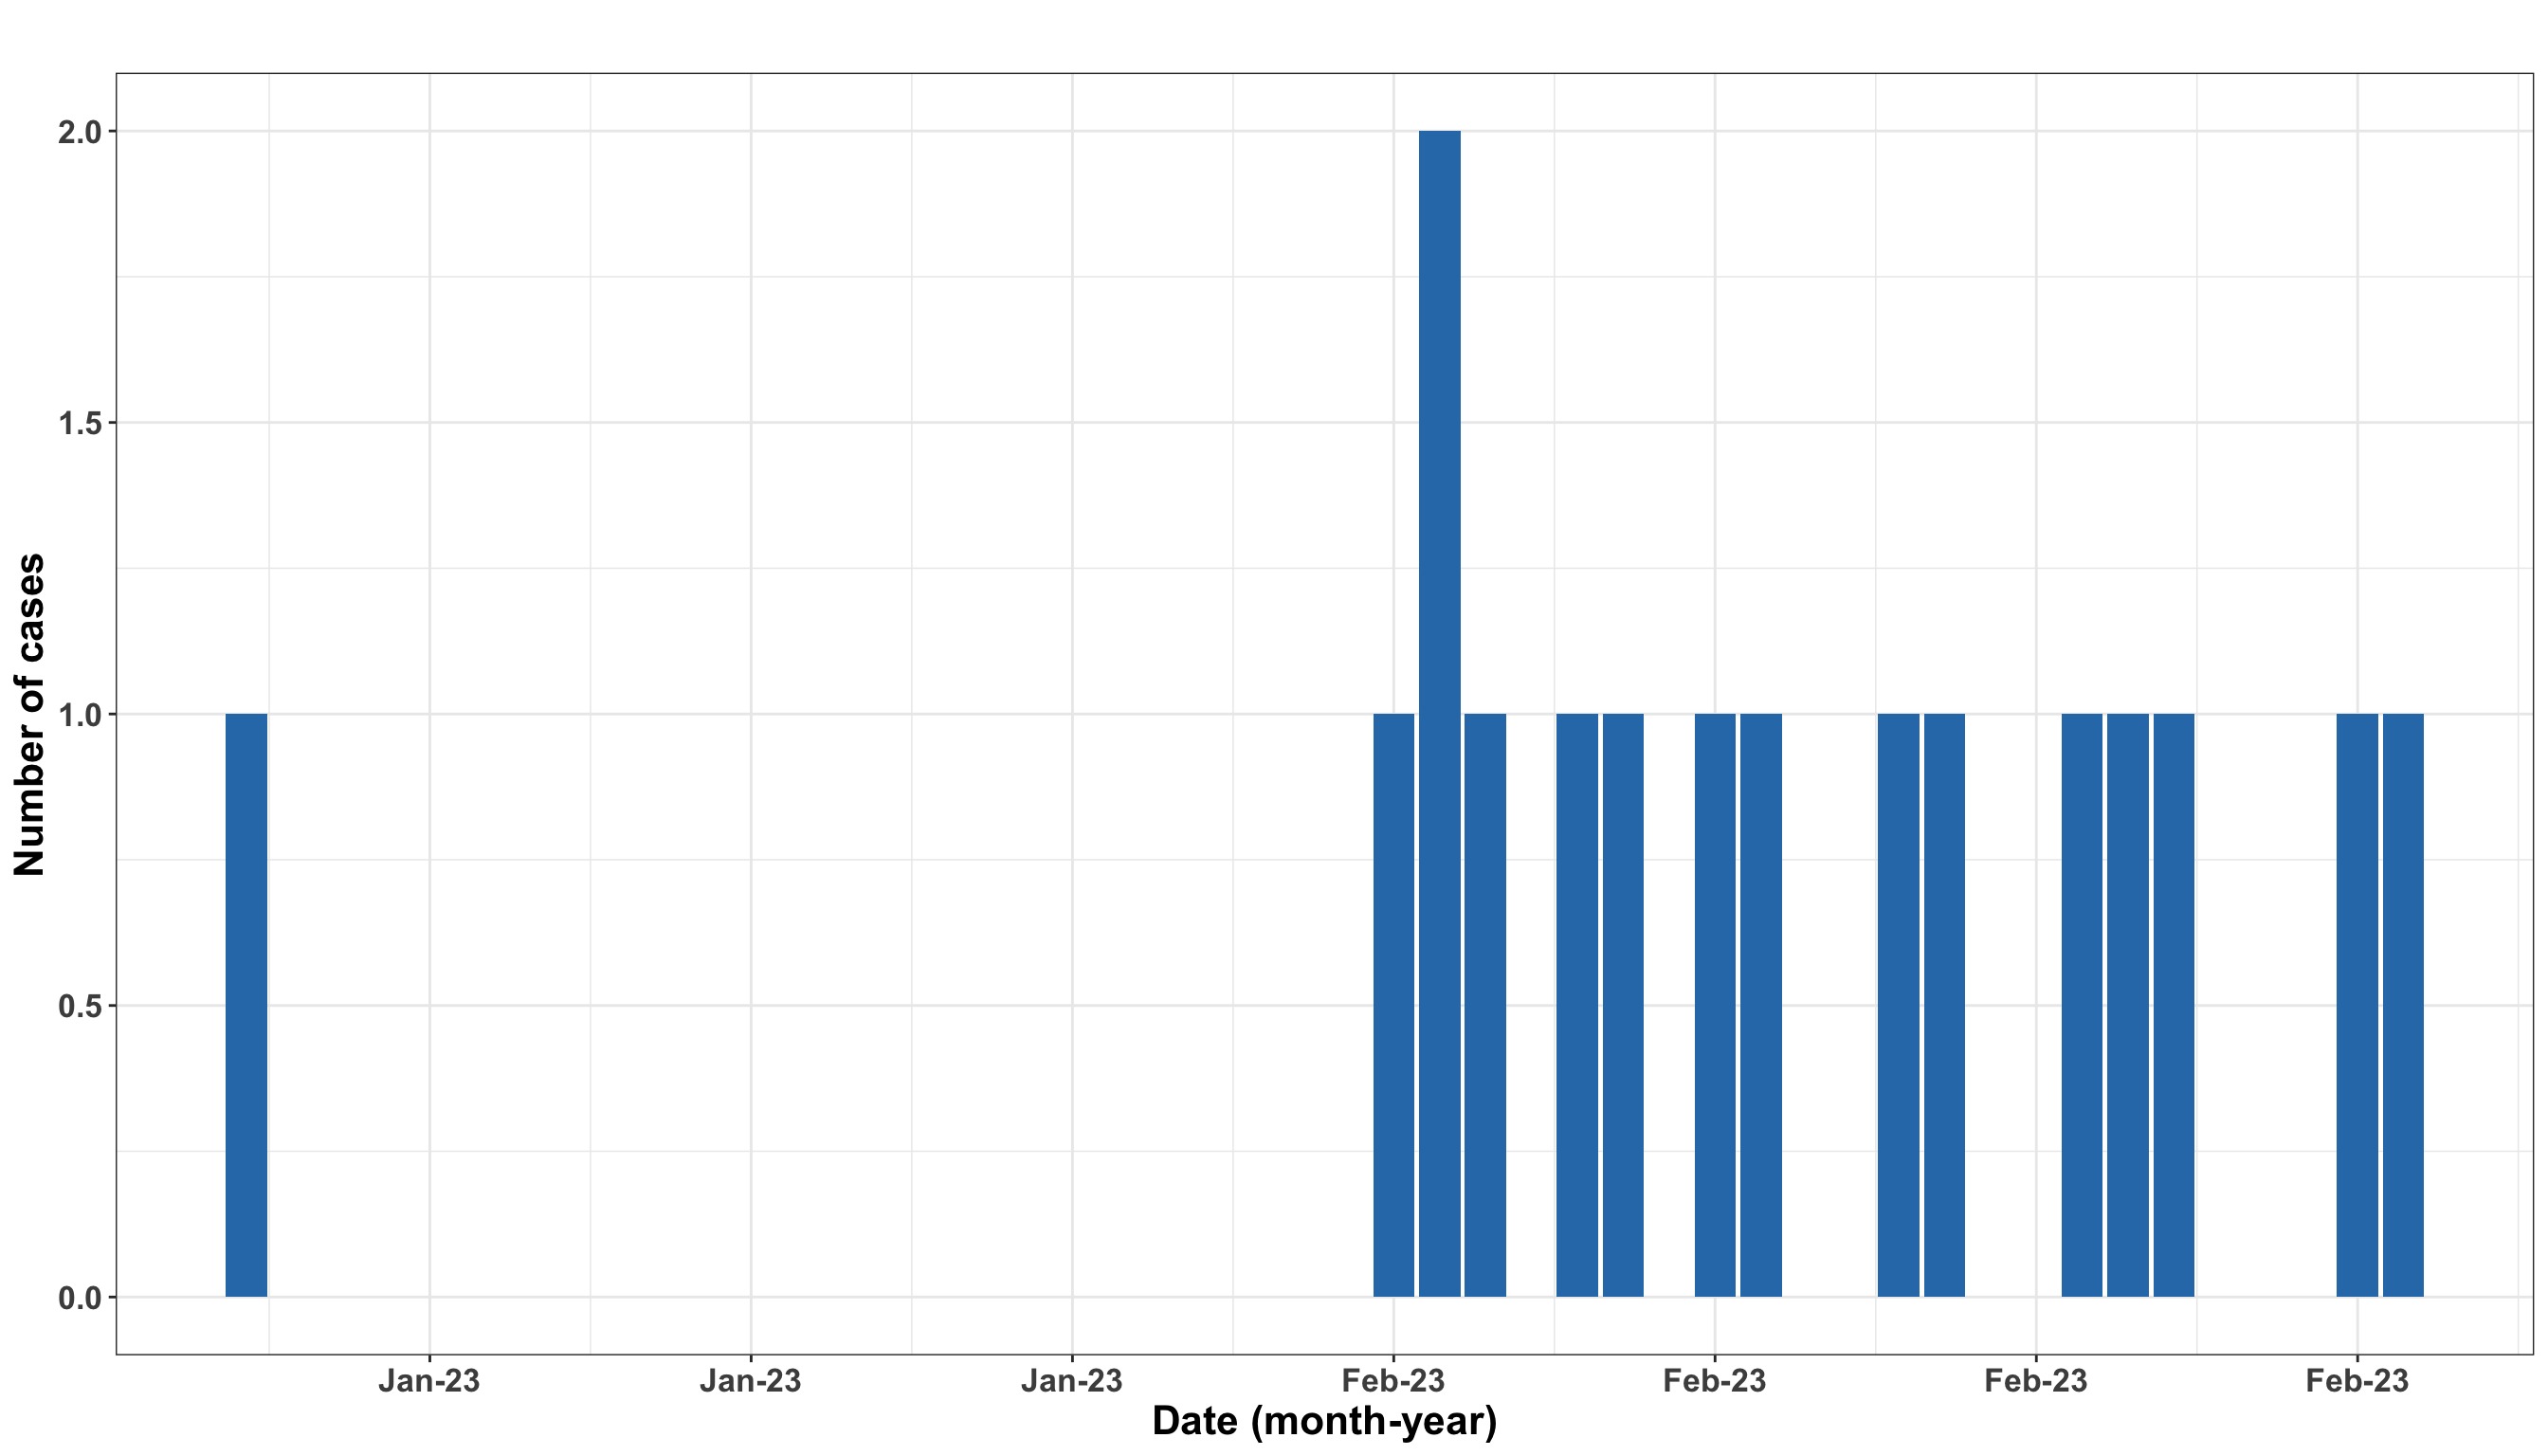
\includegraphics{_main_files/figure-latex/unnamed-chunk-106-1.pdf}

\hypertarget{demographic-distribution-17}{%
\section{Demographic distribution}\label{demographic-distribution-17}}

The stratification of these cases by age and sex is as shown:

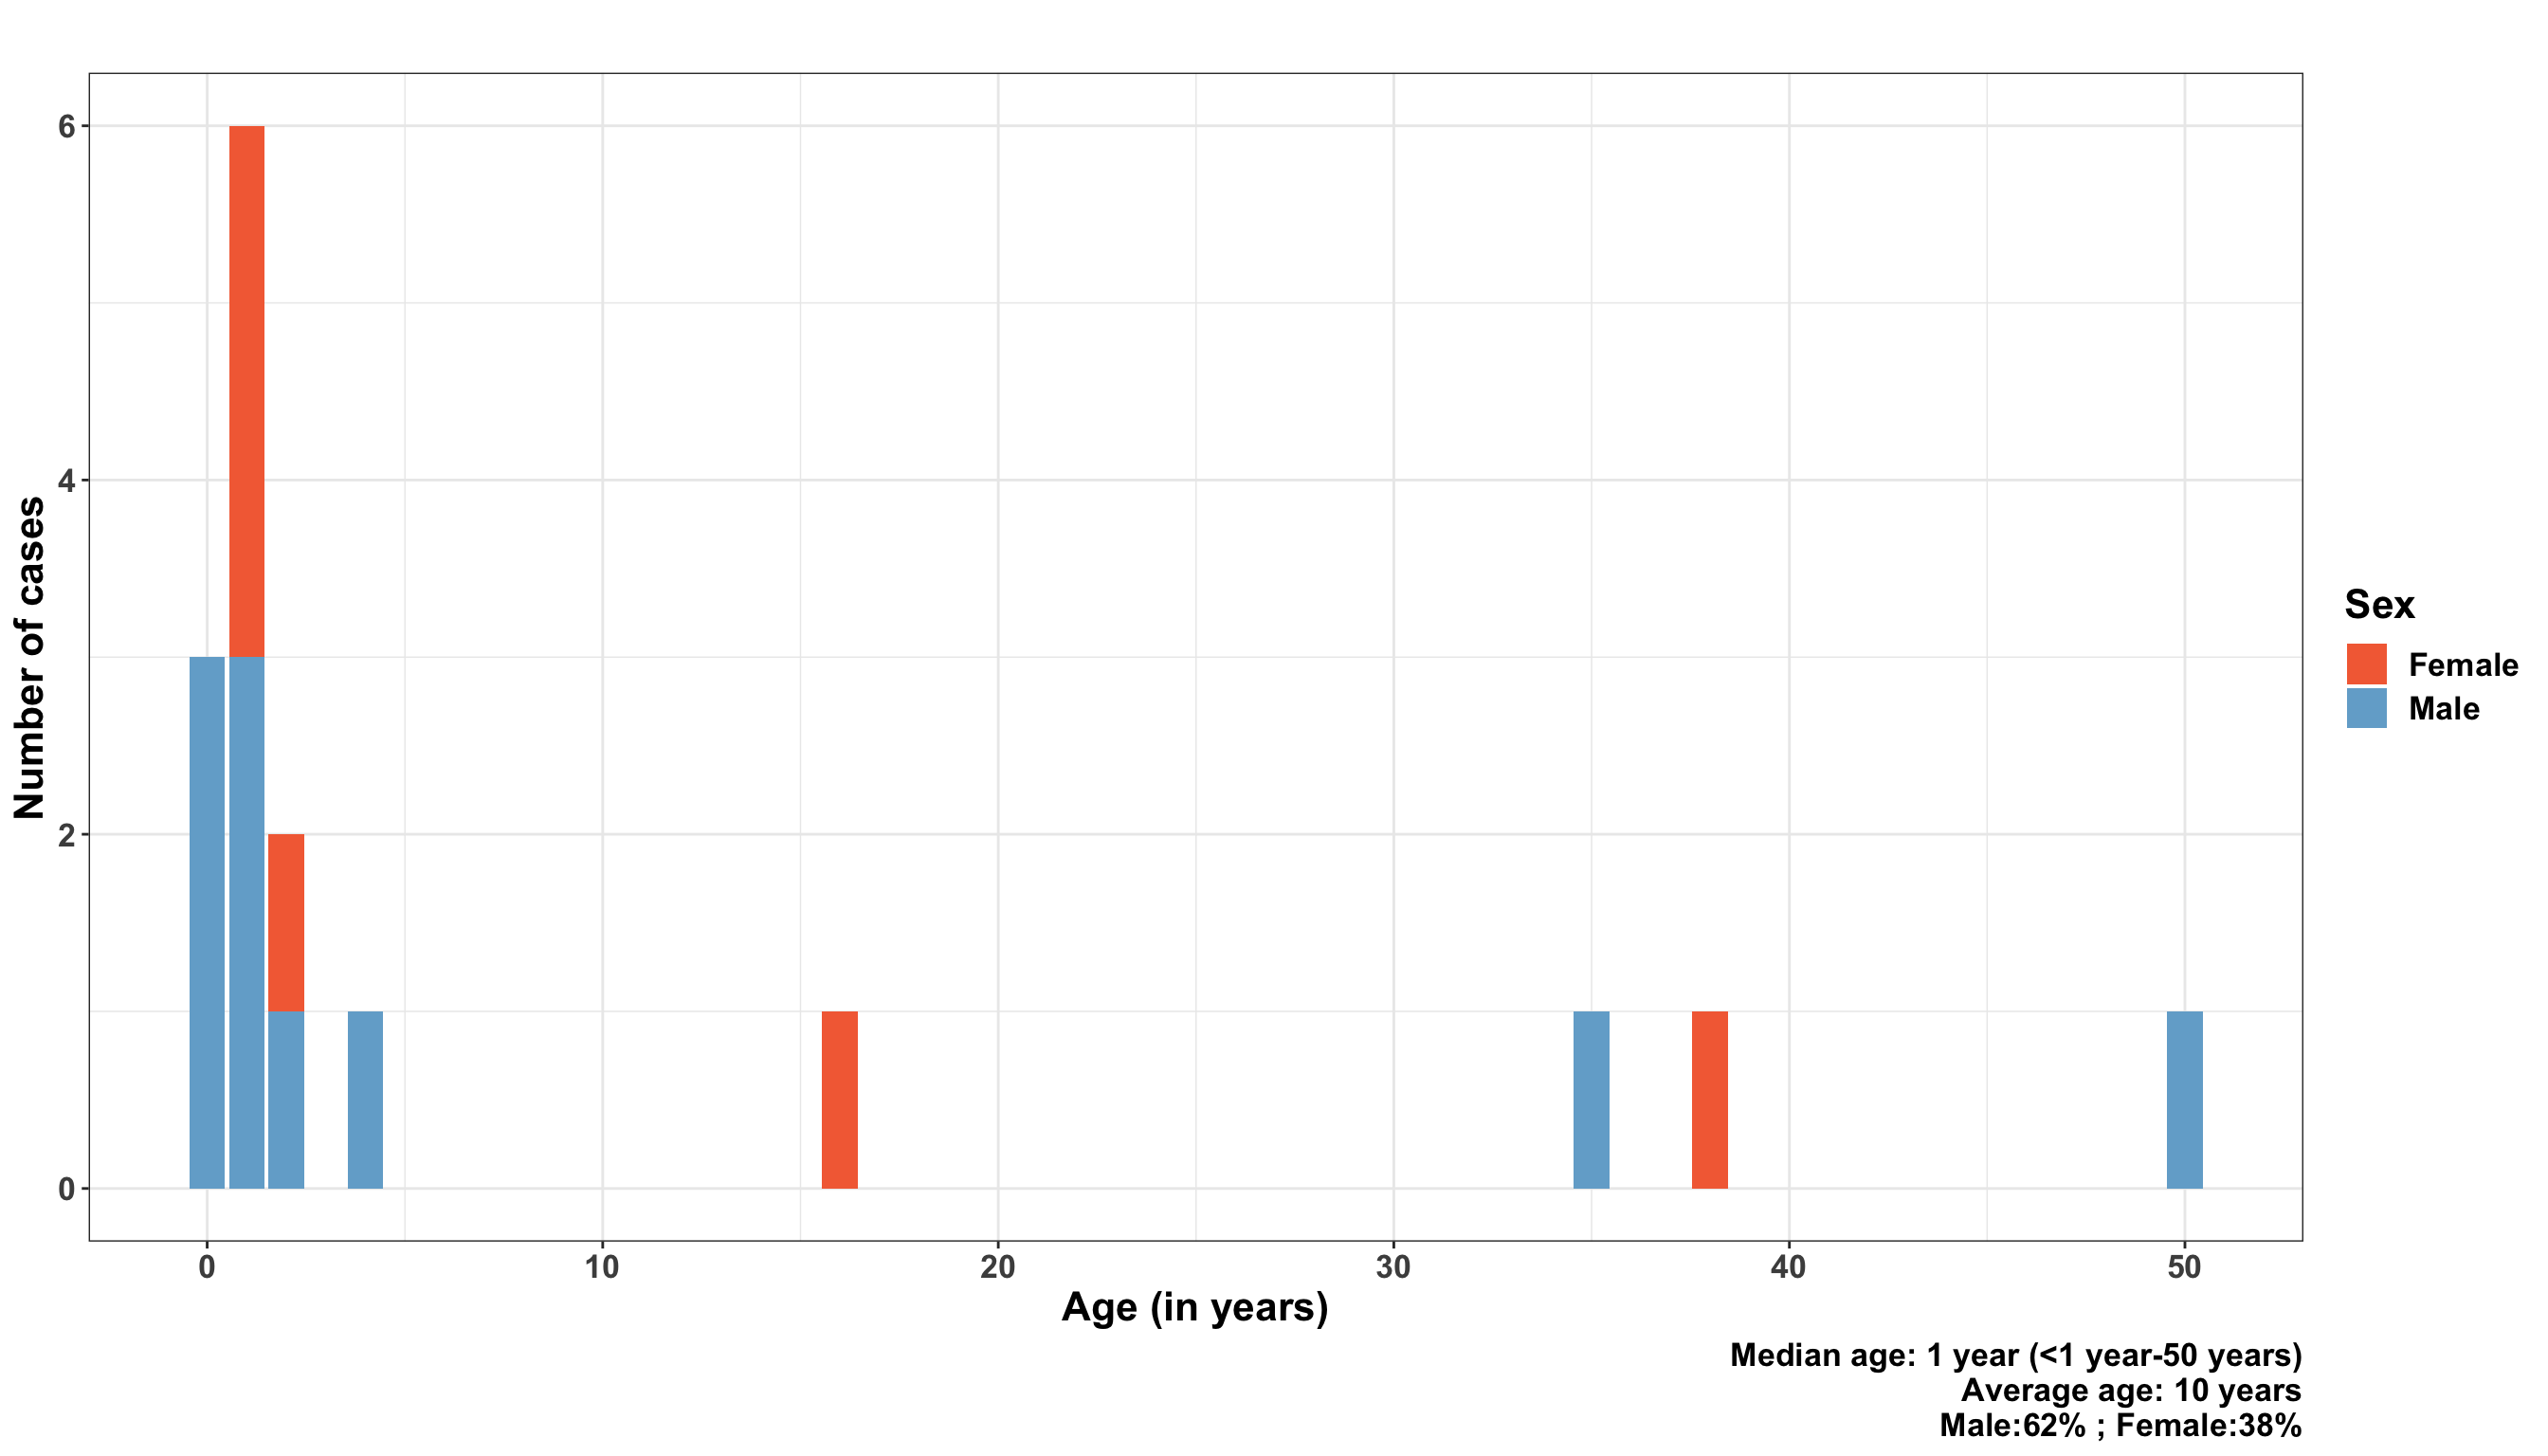
\includegraphics{_main_files/figure-latex/unnamed-chunk-108-1.pdf}

\hypertarget{spatial-distribution-17}{%
\section{Spatial distribution}\label{spatial-distribution-17}}

The spatial distribution of these cases at subcounty level is as shown:

  \bibliography{book.bib,packages.bib}

\end{document}
